\documentclass[12pt,letterpaper]{article}


%% Format (line space, space)
\usepackage[top = 1 in, bottom = 1 in, outer = 1 in, inner = 1 in]{geometry}

%% Change line space
\usepackage{setspace}
\doublespacing
\setlength{\marginparwidth}{2cm} 
%renewcommand{\baselinestretch}{1.67}
%\setlength{\footnotesep}{1.67 \footnotesep} 

\usepackage{float}


%% Add Mmakecell
\usepackage{makecell}

%% Add graphics
\usepackage{graphicx}
\usepackage[caption=false]{subfig} % Subfigures

%% Some Tikz stuff
\usepackage{tikz}
\usetikzlibrary{positioning,backgrounds,fit}

%% Bibliography (ref: Thomas Leeper)
\usepackage{natbib}
\bibpunct{(}{)}{;}{a}{}{,} %set in-line reference punctuation
\setlength{\bibsep}{0.1in} %set spacing between references
\setlength{\bibhang}{.5in} %set hanging indent for references
\newcommand\cites[1]{\citeauthor{#1}'s\ (\citeyear{#1})}
\usepackage{multibib}
\newcites{appendix}{References for Supplementary Materials}
\newcites{memo}{References for Response Memo}

%% Add hyperlinks
%\usepackage[hidelinks]{hyperref}
\usepackage[]{hyperref}
\usepackage{xcolor}
\hypersetup{
    colorlinks,
    linkcolor={red!50!black},
    citecolor={blue!50!black},
    urlcolor={blue!80!black}
}

%% Make three-part tables and adjust the width of the tables
\usepackage{threeparttable, tabularx, adjustbox}

%% Equation (for align)
\usepackage{amsmath}

%% Change counter (for Appendix)
\usepackage{chngcntr} 

%% Control layout of itemize, enumerate, description
\usepackage{enumitem}

%% Comment out a large part
\usepackage{comment}

%% Make a blind copy: 0 (not blind), 1 (blind)
\newcommand{\blind}{0}

%% Add Hypothesis
\usepackage{ntheorem}
\theoremseparator{:}
\newtheorem{hyp}{Hypothesis}
\newtheorem{q}{Question}

%% Adjustments to bullet points
\usepackage{enumitem}
\setlist{nosep}

%% Create custom epigraph environment
\newenvironment{myepigraph}
  {\par\hfill
   \begin{tabular}{@{}r@{}}} % 2em from the right margin
  {\end{tabular}\par\medskip}

  \usepackage{epigraph}

% \epigraphsize{\small}% Default
\setlength\epigraphwidth{8cm}
\setlength\epigraphrule{0pt}

\usepackage{etoolbox}

\makeatletter
\patchcmd{\epigraph}{\@epitext{#1}}{\itshape\@epitext{#1}}{}{}
\makeatother


%% Todo
\usepackage{todonotes}

% Prevent long URLs from running off the page
\usepackage{xurl}


%% Appendix
\usepackage[toc,page,header]{appendix}
\usepackage{minitoc}

% Make the "Part I" text invisible
\renewcommand \thepart{}
\renewcommand \partname{}

% To compile a LaTeX document with the table generated by the modelsummary package
\usepackage{booktabs}
\usepackage{siunitx}
\newcolumntype{d}{S[
    input-open-uncertainty=,
    input-close-uncertainty=,
    parse-numbers = false,
    table-align-text-pre=false,
    table-align-text-post=false
 ]}

 % Add checkmark
\usepackage{amssymb}

% Landscape mode
\usepackage{lscape}

% Set the numbering of tables
\makeatletter
\newcommand\setItemnumber[1]{\setcounter{enum\romannumeral\@enumdepth}{\numexpr#1-1\relax}}
\makeatother

\title{Reward or Shoot the Messenger? Experiments on How People Treat the Messenger After Receiving Good Or Bad News}
\date{}
\newcommand{\tit}{Reward or Shoot the Messenger? Experiments on How People Treat the Messenger After Receiving Good Or Bad News}
\newcommand{\da}{\today} % Manually update the date
\newcommand{\wordcount}{11,579}

\begin{document}

\if0\blind
\title{\tit}

\author{Alessandro Del Ponte\thanks{\textbf{Corresponding Author:
}~Assistant Professor, The University of Alabama. Mailing Address: 324 ten Hoor Hall, Tuscaloosa, AL 35401, USA.
Email: \href{mailto:
adelponte@ua.edu}{\texttt{adelponte@ua.edu}}.}
\and Alan S. Gerber\thanks{Sterling Professor of Political Science, Yale
University. Mailing Address: 77 Prospect Street, New Haven, CT 06511, USA. Phone:
+1 (203) 432-5232. Email: \href{mailto: alan.gerber@yale.edu}{\texttt{alan.gerber@yale.edu}}.} 
\and Gregory A. Huber\thanks{Forst Family Professor of Political Science, Yale University. Mailing Address:
77 Prospect Street, New Haven, CT 06511, USA. Phone: +1 (203) 432-5731. Email:
\href{mailto: gregory.huber@yale.edu}{\texttt{gregory.huber@yale.edu}}.} 
\and John J. Cho\thanks{Pre-Doctoral Fellow, Institution for Social and Policy Studies, Yale
University. Email: \href{mailto: john.cho@yale.edu}{\texttt{john.cho@yale.edu}}.
}}

\date{\da}
\maketitle
\fi

\if1\blind
\title{\tit}
\date{\da} 
\maketitle
\fi

\thispagestyle{empty}

\if0\blind
\newpage{}
\thispagestyle{empty}
\fi

\clearpage

\newcommand{\myabstract}{
\noindent Do people reward (RTM) or shoot the messenger (STM)? In two preregistered
experiments (N=5,200), a participant---the respondent---performed a task for
real money. Another person---the messenger---told the respondent whether
they succeeded or failed. Next, participants were matched with a partner---either the messenger or another participant. Using economic games, we measured
how prosocial respondents were toward their partner. Using rating scales, we
measured how much they liked their partner. In Experiment 1, we find both an STM
and an RTM\@. Moreover, good or bad news did not affect how respondents treated
non-messengers. In Experiment 2, we informed respondents that messengers had no
stakes in the news or earned money when participants succeeded or failed. When
messengers had no stakes in the outcome, respondents rewarded messengers when
they succeeded. When messengers had a stake in respondents' success (failure),
the STM disappeared (was exacerbated) whereas the RTM persisted.}
\clearpage

\begin{abstract}
    \myabstract
    
    \vspace{0.2in}
    \noindent \textbf{Key Words}: voter turnout; emotions; anger; field experiments\\
    \noindent \textbf{Word Count}: 11,691
    \end{abstract}
    \clearpage

\begin{epigraph}
  {How beautiful on the mountains are the feet of those who bring good news.}{Isaiah 52:7}
\end{epigraph}
  
\begin{epigraph}
  {Nobody likes the man who brings bad news.}
  {Sophocles, Antigone, Scene I, 233}
\end{epigraph}

\vspace{.5cm}

Do people treat messengers differently depending on whether they deliver
good or bad news? History offer many examples of
messengers being rewarded after bringing good news or falling in
disgrace after bearing bad news. One famous example includes
Pheidippides, who was hailed as a hero after announcing Athens' victory
in the battle of Marathon and exhaling his last breath after running 42
kilometers to deliver the news \citep{christensen2009herodotosa}.

\emph{Messenger bias}, i.e., people's tendency to reward messengers for
bringing good news and punish them for breaking bad news, is present
also in modern life and has implications for better understanding
interpersonal relationships, workplace interactions, and
politics.\footnote{Although ``messenger bias'' may encompass the
  disparate treatment of messengers on the basis of gender, race, or
  other demographic characteristics, this paper focuses on the messenger
  bias due to the valence of message content.} The inefficiencies and
large societal costs caused by this messenger bias invite studying it
and understanding how to ameliorate it. When messengers expect a bias
depending on the news they bear, whether it is positive for good news or
negative for bad news, they may act in anticipation of those effects.
For instance, employees who fear punishment for breaking bad news to
their managers may prefer to stay quiet (i.e., shooting the messenger),
threatening corporations' long-term survival \citep{charan2002companies}.
Similarly, in the wake of a disaster, politicians may downplay
responsibilities \citep{liu2020framing}, hindering efforts to prevent the
next catastrophe. At the same time, the opposite side of the messenger
bias may be just as detrimental. Rewarding the messenger who brings good
news may lead employees and politicians to focus on finding ways to be
the ones who \emph{communicate} good news rather than those who
\emph{work} toward achieving good outcomes \citep[see, e.g.,][]{grimmer2014impression}.
Throughout this paper, we label the ``shoot the
messenger'' effect as the ``STM'' effect and the ``reward the
messenger'' effect as the ``RTM'' effect.

We provide the first experimental demonstration of messenger bias using
behavioral outcomes and also confirm and extend prior results found with
attitudinal measures. We also show how the messenger bias
can be reduced. In our experiments, we use real human participant to
both receive messages and to deliver messages, a point of contrast from
prior work using confederates or a fictional character in a vignette \citep{kuhlen2013language}. In two large pre-registered experiments (Study 1 and Study 2), we compared
people's decisions toward a messenger who delivered good rather than bad
news against decisions toward another partner who was not the messenger. In
the second study, we also manipulate the messenger's payoffs depending
on the news they delivered and fully informed participants of the
messenger's incentives. The messenger earned (lost) money when the
respondent won (lost) (shared fate), lost (earned) money when the respondent
won (lost) (opposite fate), or earned nothing regardless of the outcome
(unrelated fate). In both experiments, we informed the subject that the
messenger had no control over the outcome news that they transmitted and
they delivered the news simply by clicking a button.

\begin{table}[]
\caption{Summary of our results regarding messenger bias}
\centering
\scalebox{.75}{%
\begin{threeparttable}
\begin{tabular}{@{}lll@{}}
\toprule
 & RTM & STM \\ \midrule
Study 1 (Baseline Study) & \makecell[l]{Present for some behaviors\\and all attitudes} & \makecell[l]{Present for some behaviors\\and all attitudes} \\
Study 2 (Adding Incentive Conditions) & \makecell[l]{Eliminated by unrelated fate condition\\(but only for behaviors)} & \makecell[l]{Eliminated by all fate conditions,\\and shared fate reverses it for behaviors} \\ \bottomrule
\end{tabular}%
\begin{tablenotes}[flushleft]
\scriptsize{\item[\hspace{-5mm}] \textit{Note:} Our experiments measure both behavioral outcomes and attitudinal measures. Behavioral measures include the dictator game, spin the wheel task, and the prisoner’s dilemma. Attitudinal measures include partner ratings of trustworthiness, likeability, niceness, and generosity.}
\end{tablenotes}
\end{threeparttable}
}
\label{tab:summary-results}
\end{table}

We find three new results across Studies 1 and 2, as summarized in 
Table \ref{tab:summary-results}. First, in both of our
studies, we confirm the existence of the shoot the messenger (STM)
effect, while also discovering a reward the messenger (RTM) effect. The
RTM effect is as large, if not larger, than the STM effect across both
Study 1 and Study 2. Second, we examine the implications of the
messenger bias by using behavioral measures, in addition to the
attitudinal measures that previous research has exclusively focused on.
We find that although in this context attitudinal effects appear to
correlate with behavioral outcomes, attitudinal measures overestimate
the messenger bias compared to behavioral measures. Finally, when
varying the incentives of the messenger in Study 2, we discover that
merely specifying the incentives of the messenger eliminates the STM for
both behaviors and attitudes, while the RTM effect remains remarkably
durable across various treatment conditions. Therefore, we contribute a
partial remedy that can help avoid the adverse consequences of messenger
bias in everyday life.


\emph{Messenger bias} measures how a messenger is treated as a
consequence of merely delivering a message. One side of the messenger
bias, the STM effect, has been assumed in prior work, which investigated
how belief in punishment for delivering bad news affected behavior.
Specifically, the antecedent of the messenger bias is the MUM (Mum about
Undesirable Messages) effect, which is the notion that people are
typically more reluctant to convey bad news than good news \citep{rosen1970reluctance,rosen1972fear}. 
Messengers prefer to avoid conveying bad news
because they fear backlash, especially when in public \citep{bond1987reluctance}.
 Later work found that this effect applies to a myriad
of situations in everyday life, such as doctors to patients \citep{clark1982death, sheldon1982truth, taylor1988telling}
 or politicians to voters \citep{dorling2002good,levy2014soothing}.

There is limited work directly demonstrating that messengers receive
biased treatment when they merely deliver good or bad news. The prior
work that is closest to our research is ``Shooting the Messenger''
\citep{john2019shooting}, which focused on people's dislike for messengers
who break bad news to them. Across several experiments, the authors
randomly assigned participants to receive good or bad news from a
research assistant who acted as a messenger. After they learned that
they won (if an odd number was randomly drawn) or lost, participants
rated the messenger's likeability on a 10-point scale. In other
experiments, the authors isolated several features of the STM effect:
the effect was specific to the messenger (compared to non-messengers),
was amplified when bad news was unexpected, and was mediated by
self-reported perceptions that the messenger had malevolent motives.
Finally, when the authors manipulated whether the messenger's motives
were aligned or misaligned with the participant's (but without a neutral
alignment condition), subjects reported that they liked shared alignment
messengers delivering bad news more than misaligned ones. Separately,
the same paper also found initial evidence that people like messengers
who bring good news, although they did not explicitly identify a RTM
effect.

Several explanations have been offered for the messenger bias. As \citet{john2019shooting}
 found, the respondent may shoot the messenger for bringing
bad news by assuming them to have malevolent motives or in a desire to
make sense of the news by blaming the messenger as the most proximate
cause. One relevant set of studies have established that criticisms, or
negative news, from out-group members are treated more harshly compared
to those by in-group members (the intergroup sensitivity effect)
\citep{hornsey2002it,esposo2013shooting}. Therefore, messengers who
bring bad news may be penalized if they are assumed to be acting counter
to the interests of the group. At the same time, this implies that
clarifying the relationship between the messenger and the recipient of
the message may be a fruitful strategy to ameliorate the messenger bias.
Specifically, the messenger showing themselves to be unaligned with any
potential out-groups may reduce the negative effect of criticisms
\citep{hornsey2007groupdirected}.

\begin{table}[]
\caption{Comparison of our work and \citet{john2019shooting}}
\label{tab:previous-work}
\resizebox{\textwidth}{!}{%
\begin{threeparttable}
\begin{tabular}{@{}lll@{}}
\toprule
 & Behavioral Measures & Attitudinal Measures \\ \midrule
Shoot the Messenger Effect & Present Research & Exp. 1, 2A, 2B, 3A, 3B, 4, 5A, 5B, 5C, 6A, 6B \citep{john2019shooting} \\
Reward the Messenger Effect & Present Research & Exp. 2A (N = 150) and 5A (N = 304) \citep{john2019shooting} \\ \bottomrule
\end{tabular}%
\begin{tablenotes}[flushleft]
\scriptsize{\item[\hspace{-5mm}] \textit{Note:} Although one experiment (2A, N=150) in John et al. (2019) did include a 2 x 2 design varying a messenger vs. a non-messenger and good vs. bad news like our experimental conditions, they do not calculate the RTM effect nor is the study well-powered to detect differences between the STM and RTM effects. The other experiment (5A, N = 304), does include a neutral message condition to assess valence effects, but no non-messenger conditions necessary to measure the STM and RTM effects.}
\end{tablenotes}
\end{threeparttable}
}
\end{table}


Taken together, the research on the STM effect and the MUM effect
suggests that messenger bias can impose tangible costs on modern society
because messengers who tell bad news are disliked and thus prefer to
stay quiet. Table \ref{tab:previous-work} summarizes the prior work and shows how our work
contributes the current literature in two ways.


Several important questions remain unaddressed in prior work. First, it
remains unknown whether attitudes toward the messenger are accompanied
by behavioral consequences. Prior work measured
\emph{attitudes} toward the messenger (especially
likeability and competence). Ultimately, uncovering whether messengers'
news may affect altruism, cooperation, and trust toward them carries
fundamental implications for understanding the information environment.
It remains unknown whether messengers' reluctance to speak out is
justified by actual repercussions against them that go beyond mere
dislike. Previous literature indicates that behavior does not
necessarily track attitudes when it interferes with self-interest and
financial incentives \citep{crano2006attitudes,lehman2002pervasive}.
(And, in equilibrium, the tendency to obscure bad news means that it is
less frequently observed, making it difficult to generate unbiased
inferences about the effect of sending bad news for non-experimental
observations.) In this paper, we address this question and build upon
\citet{john2019shooting} by studying how people treat messengers after
receiving good news or bad news from them using incentivized
experiments. Since we have both behavior and attitudinal measures in the
same studies, we can directly compare the performance of these measures.

Second, our experimental design addresses some issues in prior work.
Such work does not fully identify the composition of the messenger bias
because of their experimental designs, which only compare reactions to
messengers bringing bad news to messengers bringing good news. Our paper
adds a ``messenger vs. non-messenger'' condition to all our
experiments in addition to the ``good news vs. bad news'' conditions.
This allows for two benefits. First, we more accurately identify the
\emph{shoot the messenger} effect (i.e., the negative reaction to a
messenger delivering bad news compared to a non-messenger) as something
distinct from the \emph{valence} effect (i.e., the negative reaction to
receiving bad news generally compared to receiving good news). Because
previous studies do not distinguish between these two effects, it
remains unclear whether there is something distinct about the
\emph{delivery} of bad news which is specific to the messenger from just
bad news generally. The second benefit is the ability to estimate the
opposite side of the messenger bias: rewarding the messenger for
delivering good news. Although previous work has not pointed out the
existence of a RTM effect, perhaps because they assume it to simply be
symmetric to the STM effect, we compare the magnitude and persistence of
these two effects. The Methods section details how we define and analyze
these quantities of interest differently from past work.

\section{Results}

\begin{figure}  
\centering{
\resizebox{1\textwidth}{!}{
\begin{tikzpicture}
\node (r1) [draw=black, dashed, fill=lightgray!30, minimum width=8.15cm,minimum height=7.5cm] at (9,0){};
\node (r3) [draw=black, dashed, fill=lightgray!30, minimum width=4.25cm,minimum height=7.5cm] at (16.5,0){};
\node (r1Label)[above=.67cm of r1] {\textbf{Part 2: Behavioral Games}};
\node (r2) [draw=black, dashed, fill=lightgray!30, minimum width=1.75cm,minimum height=7.5cm] at (3,0){};
\node (r2Label)[above=0cm of r2] {\textbf{  \begin{tabular}{c}
     Part 1: Perform Task\\
     and Receive Message\\
  \end{tabular} }};
\node (r3Label)[above=.58cm of r3] {\textbf{After Part 2 Complete}};
\node[shape=rectangle, draw] at (0,0) {SUBJECT};
\node[shape=rectangle, draw,  align=left] at (3,2) (win) {Win\\Message};
\node[shape=rectangle, draw,  align=left] at (3,-2) (loss) {Loss\\Message};
\node[shape=rectangle, draw, align=left] at (6,3) (messenger_win) {Play with:\\Messenger};
\node[shape=rectangle, draw, align=left] at (6,1) (stranger_win) {Play with:\\Stranger};
\node[shape=rectangle, draw,  align=left] at (6,-1) (messenger_loss) {Play with:\\Messenger};
\node[shape=rectangle, draw, align=left] at (6,-3) (stranger_loss) {Play with:\\Stranger};
\node[shape=rectangle, draw] at (10,3) (bg) {\textbf{Behavioral Measures}};
\node[shape=rectangle, draw] at (10,2) (dg) {Dictator Game};
\node[shape=rectangle, draw] at (10,0) (stw) {Spin the Wheel};
\node[shape=rectangle, draw] at (10,-2) (pd) {Prisoner's Dilemma};
\node[shape=rectangle, draw] at (16.5,3) (am1) {\textbf{Attitude Measures}};
\node[shape=rectangle, draw] at (16.5,2) (trust) {Trustworthy};
\node[shape=rectangle, draw] at (16.5,.66) (nice) {Nice};
\node[shape=rectangle, draw] at (16.5,-.66) (like) {Likeable};
\node[shape=rectangle, draw] at (16.5,-2) (generous) {Generous};


\draw[->] (0.5,0.5) -- (win.west) node[midway,above] {};
\draw[->] (0.5,-0.5) -- (loss.west) node[midway,below] {};
\draw[->] (win.east) -- (messenger_win.west) node[midway,above] {$\frac{1}{2}$};
\draw[->] (win.east) -- (stranger_win.west) node[midway,below] {$\frac{1}{2}$};
\draw[->] (loss.east) -- (messenger_loss.west) node[midway,above] {$\frac{1}{2}$};
\draw[->] (loss.east) -- (stranger_loss.west) node[midway,below] {$\frac{1}{2}$};
%\draw[->] (dg.south) -- (stw.north) node[midway,below]{};
%\draw[->] (stw.south) -- (pd.north) node[midway,below]{};
\end{tikzpicture}
}
}
\caption{Survey Flow of Study 1 and 2.\label{fig:survey-flow} \textit{Note:} 1/3 of attitude measures were asked after receiving the message in Part 1, while the other 2/3 were asked after Part 2. In our analysis, we group whether attitude measures were asked before or after Part 2. Subjects learn results of behavioral games after all outcome variables (behavioral and attitudes) are concluded.}
\end{figure}

We conducted two related experiments that investigate the messenger bias
in attitudes and behaviors. Figure \ref{fig:survey-flow} shows the experimental design for
both Study 1 and Study 2. In both studies, participants performed an
incentivized task (either the ``counting task,’’ counting odd numbers in a matrix, emulating ``skill,'' or the ``prediction task,’’ predicting a coin toss, emulating luck) with a
small bonus if they ``win'' the task in the first round. Then, they
were informed by a messenger (who is another real participant who did
not perform the task) about the outcome (win or lose) in the first
round. Respondents were informed that the messenger had no agency over the
message and ignored its content: they could only click a button to
deliver the news. Finally, we measured respondents' attitudes and
behaviors toward the messenger and compared them to the attitudes and
behavior toward another participant who was not the messenger when the
same news had been delivered. We tested three different behavioral
measures aimed at capturing altruism (the dictator game), cooperation
(prisoner's dilemma), and participants' intuitions about the messenger's
likelihood to bring good news in an unrelated task (spin the wheel
task). We also measure four attitudinal measures similar to those used
in prior work: the partner's trustworthiness, likeability, niceness, and
generosity. Study 2 builds on Study 1 by following a similar design,
except that we also manipulated whether the messenger's payoffs were
aligned with, unrelated to, or opposite to the participant's. Respondents
were fully informed about the messenger's payoffs relative to the news
they conveyed. Depending on the condition, when a participant won, the
messenger also earned some money (shared fate conditions), earned
nothing (unrelated fate condition), or lost money (opposite fate
condition). We analyze each behavioral and attitudinal measure
separately using OLS regression with robust standard errors.

Across both studies, we estimate the RTM and STM effects for each of the behavioral and attitudinal
measures, along with detailing messenger bias and the relative magnitude
of the RTM and STM effects. The STM effect is shown on the left-hand side of each panel and it is calculated by comparing behaviors and attitudes towards the messenger from the non-messenger, after losing the first task. 
Similarly, the RTM effect is on the right-hand side of each panel and is estimated for those who won the first task.
We also compare the relative magnitude of these two estimates by testing
whether $RTM = -STM$ (not shown, only described in the footnote of
the figure). Finally, we claim that a messenger bias exists if we fail to
reject the joint hypothesis test that $STM = 0$ and $RTM = 0$ (not
shown, only described in the footnote of the figure). The Methods section
provides additional details on how we define these quantities of
interest.

\subsection{Study 1}

First, we examine respondents' decisions for the behavioral measures in Figure \ref{fig:behavior_list}: how
much money is shared in the dictator game, who is chosen to spin the
wheel, and whether the respondent chooses to cooperate or defect in the
prisoner's dilemma game.\footnote{The corresponding coefficients for
 the respective regressions for Figures \ref{fig:behavior_list} (for behavioral measures) and \ref{fig:attitude_list} (for attitudes measures) are seen in Tables \ref{tab:behavior_regression} and \ref{tab:attitude_regression}, respectively, in
 Appendix \ref{sec:appendix_study1}.} Recall from Figure \ref{fig:survey-flow} that following winning or
losing the first stage, respondents were randomly assigned to play
behavioral games with either the individual who delivered the message in
part 1 (messenger treatment) or a new partner unrelated to the messenger
(non-messenger treatment).

\renewcommand{\baselinestretch}{1.25}%
\begin{figure}[!t]%
  \centering
  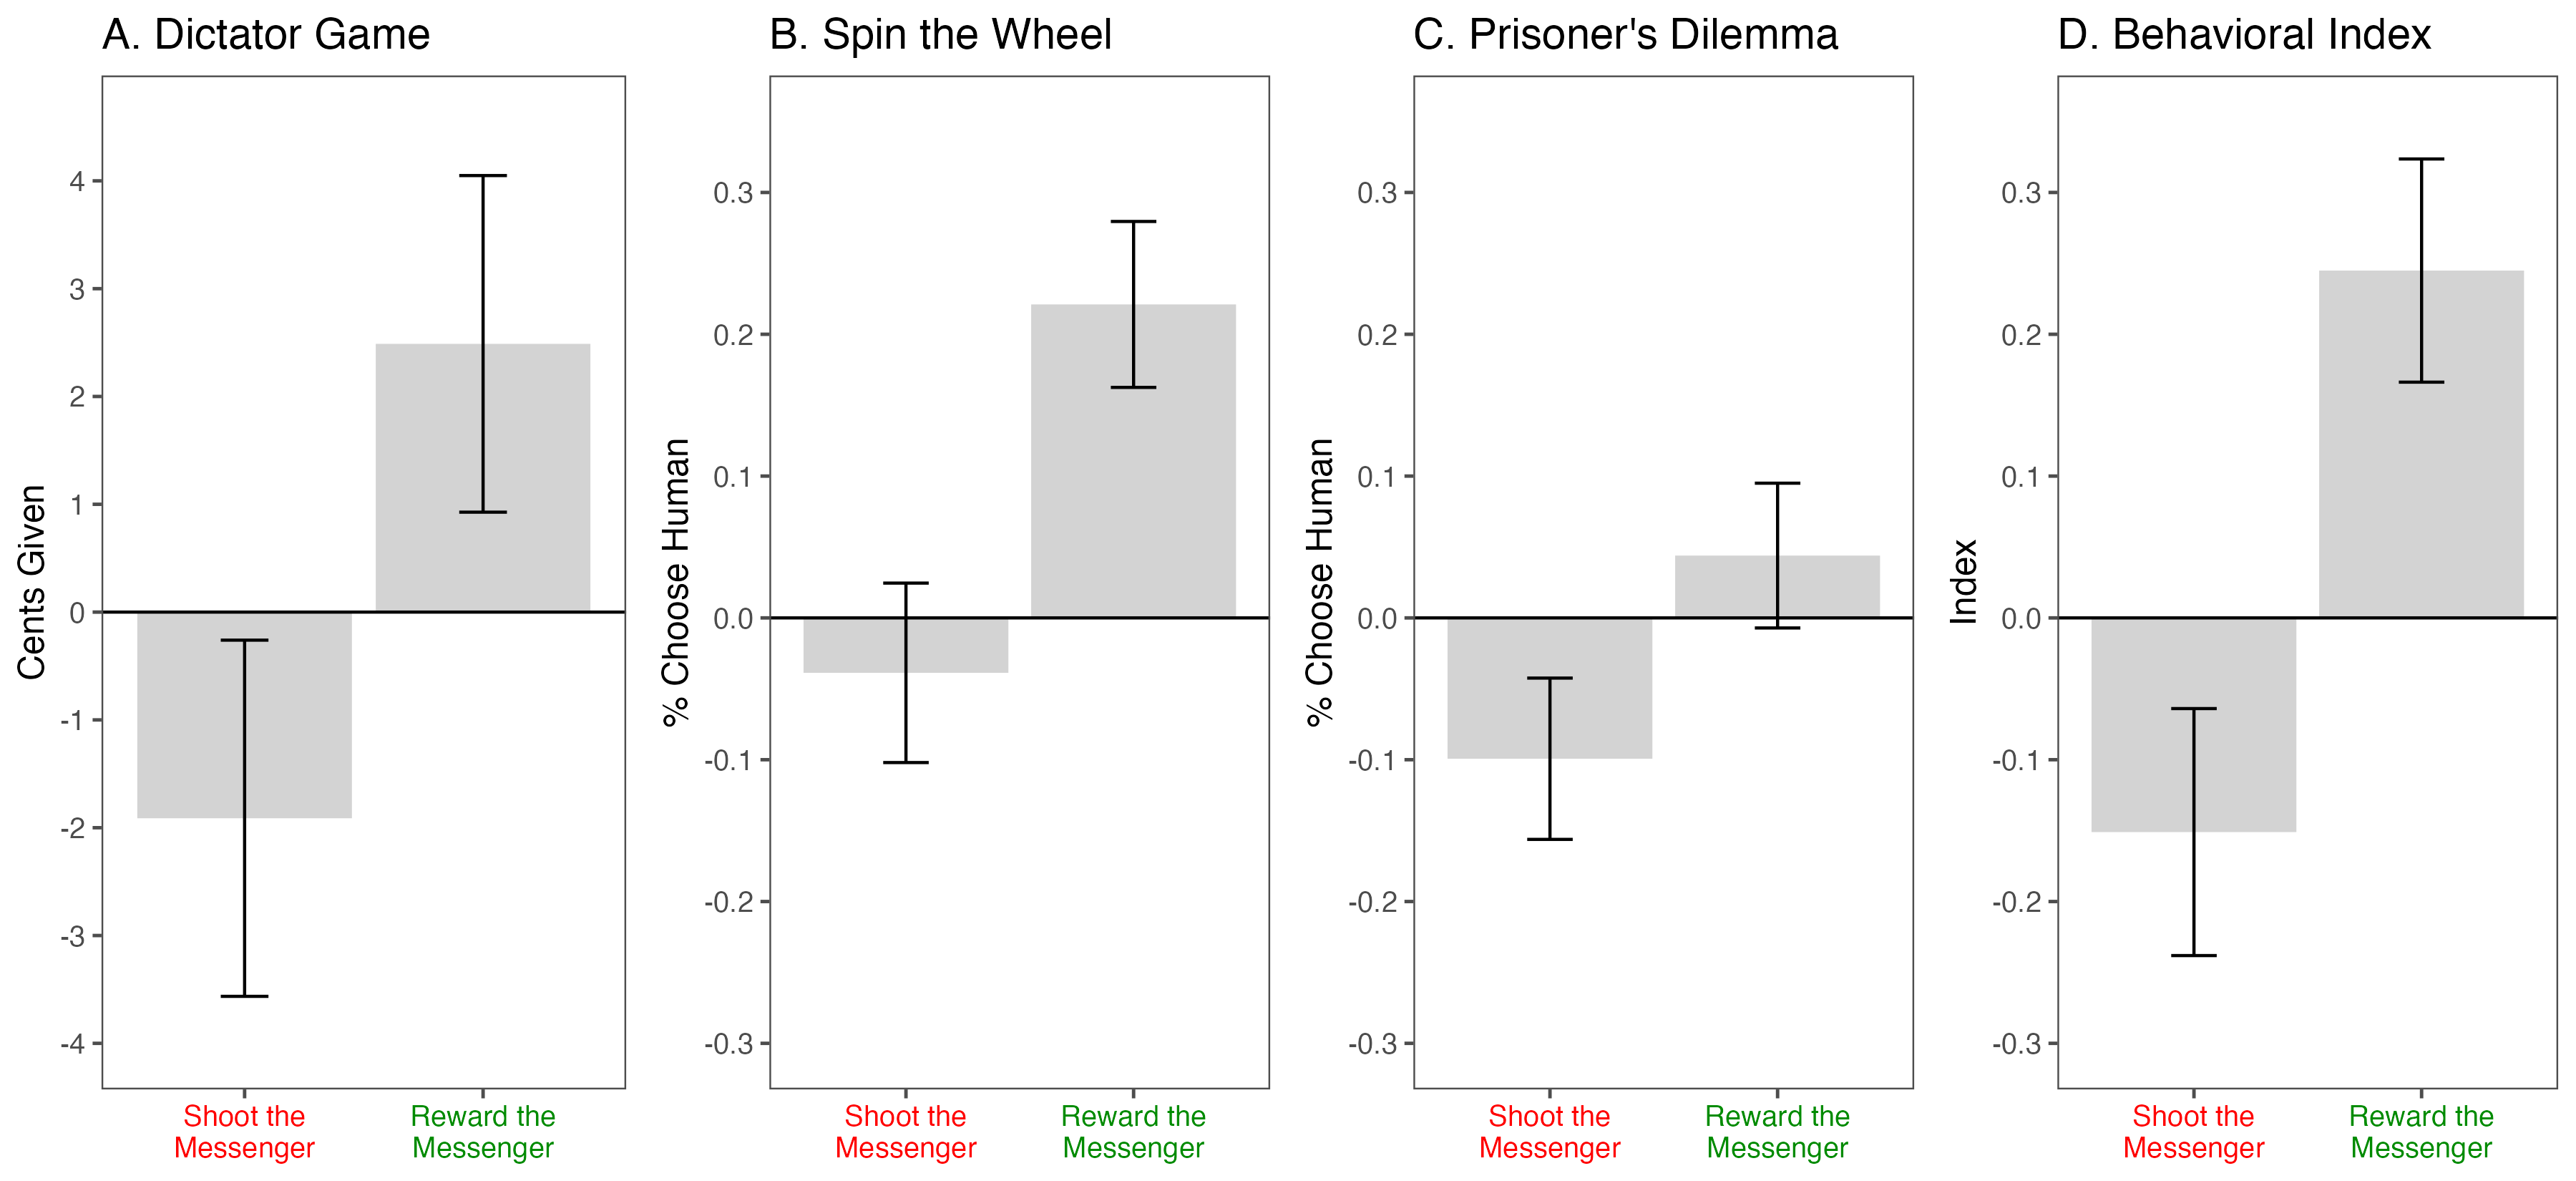
\includegraphics[width=1.0\textwidth]{figures/study1_behavior_list.png}
  \caption{Difference in the DVs of the behavior measures for messengers and non-messengers 
                                              by losing (STM) and winning (RTM), Study 1. 
  \textit{Note: OLS regression with robust standard errors, with error bars representing 95\% confidence intervals. In the dictator game (Panel A), the dependent variable (DV) is giving up to 50 cents to the partner. 
                 In the spin the wheel task (Panel B), the DV is choosing the partner to spin the wheel on one’s behalf instead of the computer. 
                 In the prisoner’s dilemma (Panel C), the DV is choosing cooperation. 
                 In the behavioral index (Panel D), the DV is calculated by averaging the standardized scores of the dictator game, spin the wheel task, and prisoner's dilemma. The p-values of the test that $RTM = -STM$ are 0.62, 0.00, 0.16, and 0.12, respectively, for each facet and the index. The p-values of messenger bias are 0.00, 0.00, 0.00, and 0.00, respectively, for each facet and the index.}}
  \label{fig:behavior_list}
\end{figure}%
\renewcommand{\baselinestretch}{1.67}%


Across all three behavioral measures, we see consistent evidence of a
messenger bias, which means participants treat messengers differently
compared to non-messengers holding constant whether the respondent wins or
loses. However, whether this bias is a result of shooting or rewarding
the messenger differs based on the specific behavioral game that the
respondents play. To start, we analyze the results of the dictator game,
where respondents could give between 0 and 50 cents to their partner
(Figure \ref{fig:behavior_list}, Panel A). We compare allocations by respondents after
winning rather than losing in decisions toward messengers and
non-messengers. When participants lost rather than won in task 1, they
sent messengers 1.91 cents less ($p < .05$) than
non-messengers, indicating that respondents ``shot the messenger''
when losing. By contrast, winning also significantly affected respondents'
behavior toward messengers compared to non-messengers (coefficient for
RTM = 2.49, $p < .01$). The difference in the relative
magnitude of these two estimates is not significant ($p =
.62$).

Next, we look at results from the spin the wheel task (Figure \ref{fig:behavior_list}, Panel B). Unlike the dictator game, we do not detect a STM effect, as 
respondents were only 4 points less likely to choose the messenger following
a first stage loss ($p = .23$). But the RTM effect persists, as when
they won in task 1, respondents were 22 points (47\%) more likely to
choose the messenger (70\%) than another participant
(48\%) ($p < .001$). We find significant
evidence of a stronger RTM effect compared to the STM effect ($p < .001$).

Finally, we look at respondents' decisions in the prisoner's dilemma
(Figure \ref{fig:behavior_list}, Panel C). When they lost in task 1, respondents were
10\% less likely to cooperate with the messenger compared to a
non-messenger ($p < .001$), providing evidence of a STM
effect. When they won in task 1, respondents were 4\% more likely to
cooperate with the messenger (79\%) than with another participant
(75\%), but this RTM effect is not significant ($p < .1$).
The difference in absolute size of these effects is not statistically
significant.

Grouping all of the behavioral measures into one combined index in
Panel D of Figure \ref{fig:behavior_list} (which we term the ``behavioral index,''
calculated as the average of the standardized behavioral measures
ranging from 0 to 1) we see an overall
STM effect of .15 and an RTM effect of .25 (both coefficients are
significant at the $p < .001$) level, which implies that
a messenger bias exists from both shooting and rewarding the messenger
($p < .001$). Although the RTM point estimate has a larger
magnitude than the STM effect, this difference is not significant ($p
= .12$). These results do not change when we include
demographic controls (Table \ref{tab:behavior_regression_demographic}).
\footnote{Along with demographic covariates such as age, gender, ideology,
education, employment, and race, we also include three psychological scales that may be
related to the messenger bias or our outcome measures. These are the just world
scale \citep{lipkus1991construction}, the emotion regulation scale \citep{buss1992aggression}, and the
belief in luck scale \citep{darke1997belief}.}
\renewcommand{\baselinestretch}{1.25}%
\begin{figure}[!t]%
  \centering
  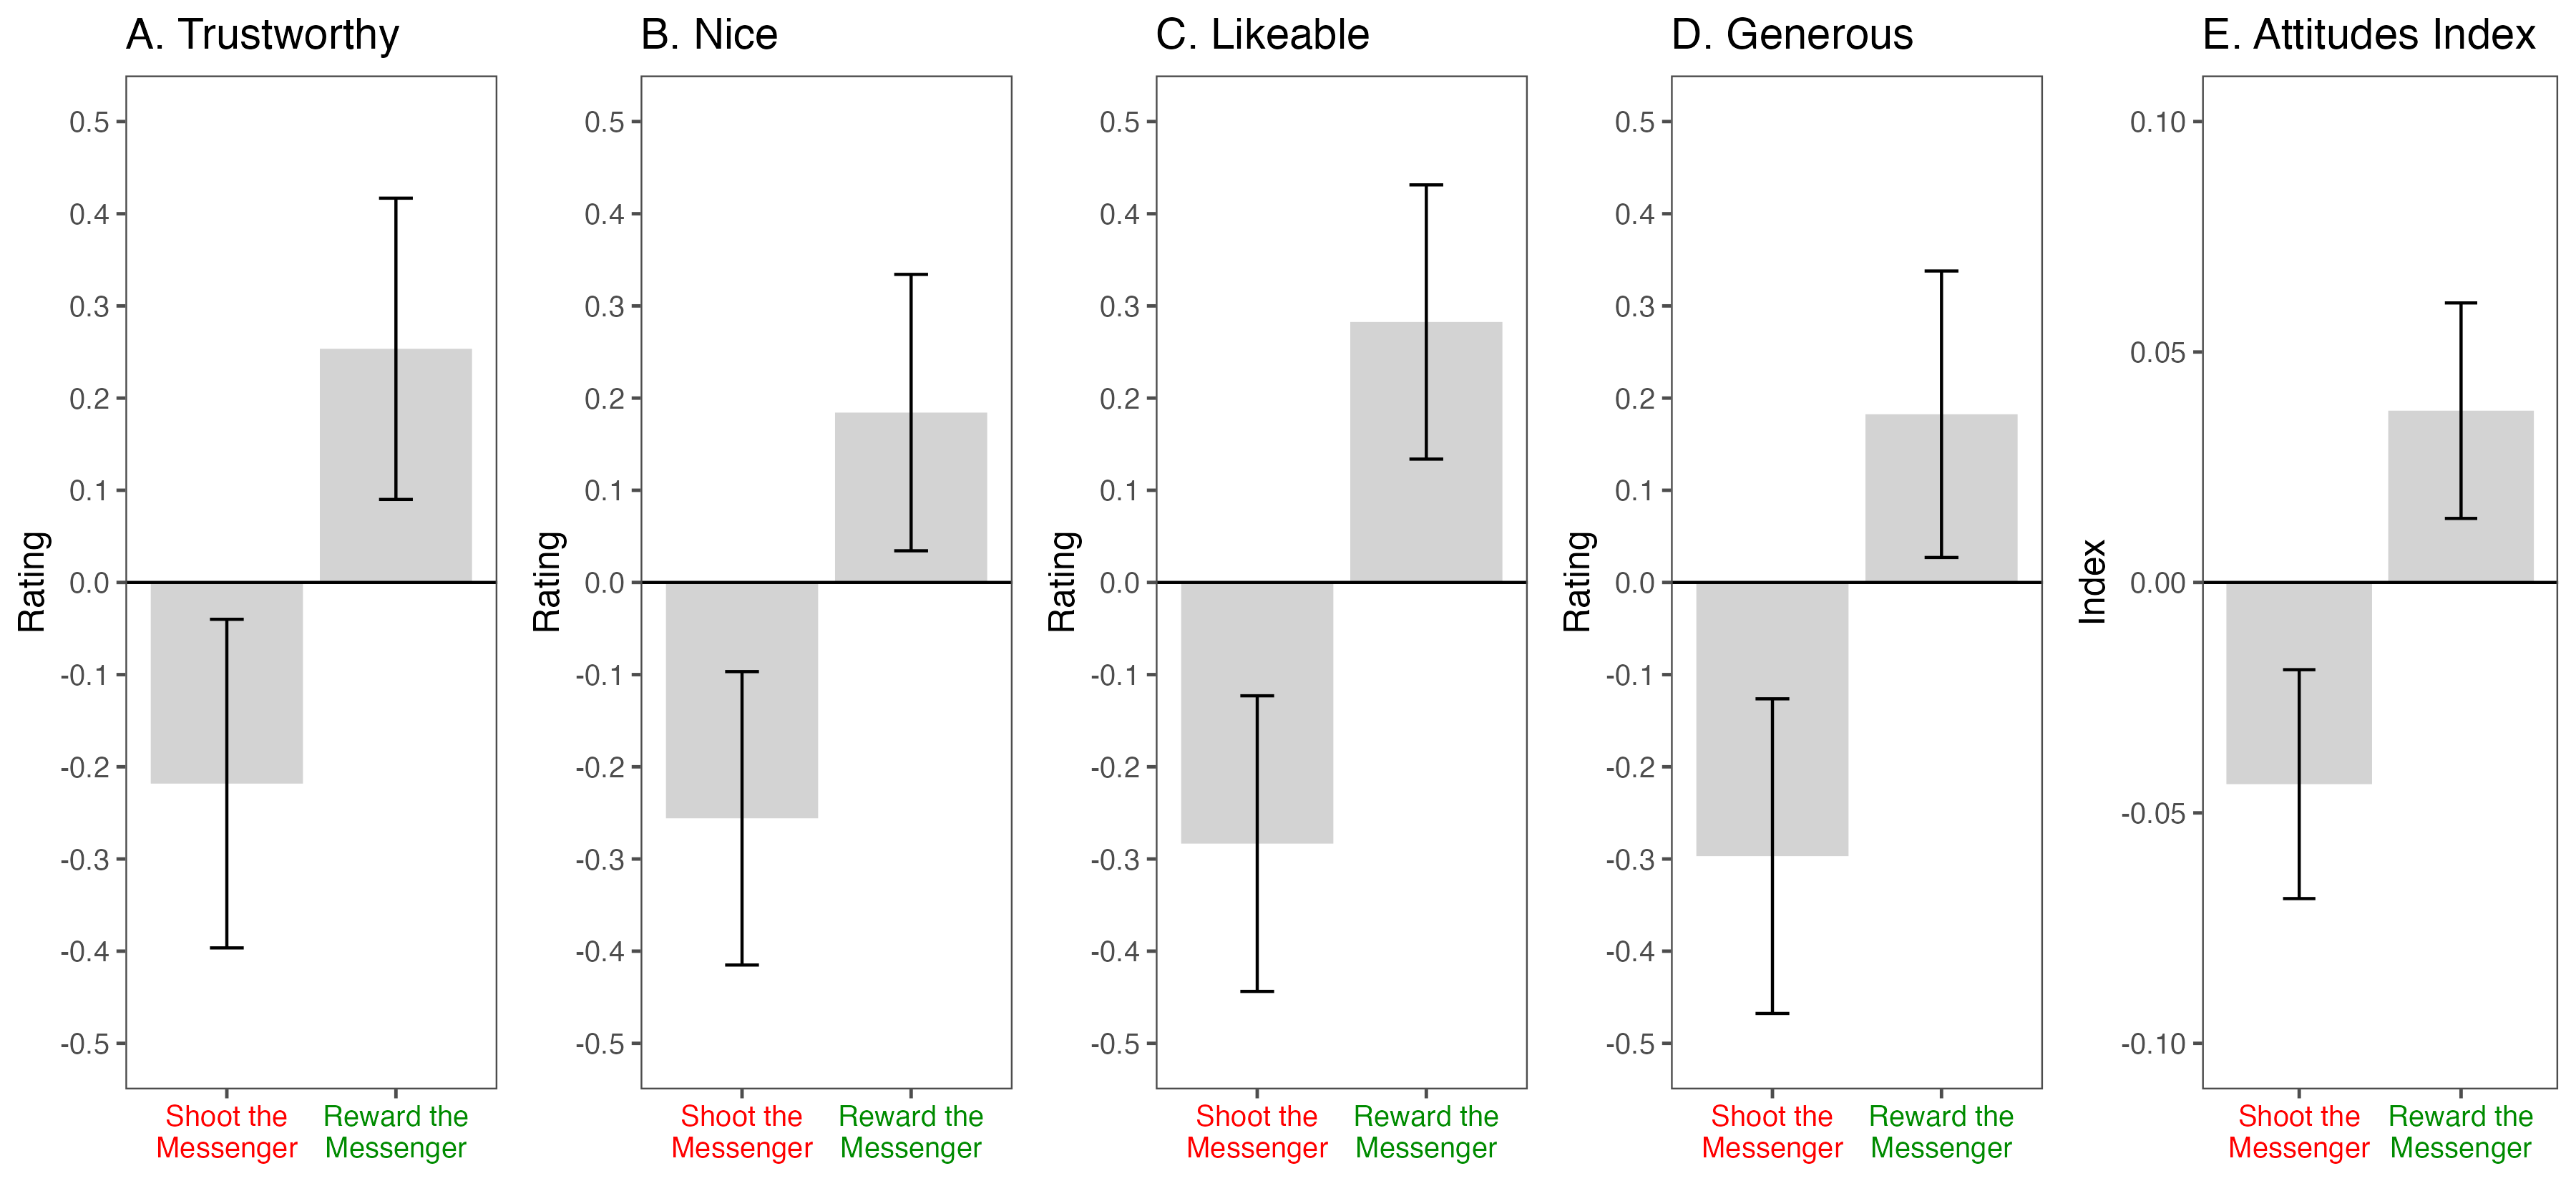
\includegraphics[width=1.0\textwidth]{figures/study1_attitude_list.png}
  \caption{Difference in the DVs of the attitude measures for messengers and non-messengers 
                                              by losing (STM) and winning (RTM), Study 1. 
  \textit{Note: OLS regression with robust standard errors, with error bars representing 95\% confidence intervals. The trustworthy (Panel A), nice (Panel B), likeable (Panel C), and generous (Panel D) dependent variables asks respondents to rate these messenger's characteristics on a 7-point Likert scale, where a score of 1 indicates that the messenger does not have that trait at all, while a score of 7 means that a trait describes the messenger extremely well.
    In the attitudes index (Panel E), the DV is calculated by averaging the ratings of the trustworthy, nice, likeable, and generous DVs to an index ranging from 0 to 1. The p-values of the test that $RTM = -STM$ are 0.77, 0.52, 0.99, 0.33, and 0.71, respectively, for each facet and index. The p-values of the messenger bias are 0.00, 0.00, 0.00, 0.00, and 0.00, respectively, for each facet and the index.}}
  \label{fig:attitude_list}
\end{figure}%
\renewcommand{\baselinestretch}{1.67}%


Next, we analyze the four attitudinal measures (trustworthiness,
niceness, likability, and generosity). Figure \ref{fig:attitude_list} presents the results
graphically, following the same logic as Figure \ref{fig:behavior_list}. Each of these
attitudes was measured on a 7-point scale. Unlike the behavioral
measures, we see consistent messenger bias, both RTM and STM effects,
across all attitudinal measures. For simplicity, therefore, we focus on
the index measure (called the ``attitudes index,'') which averages the
 ratings of the four attitudes from 0 to 1. We
see that respondents consistently rewarded the messenger, as they are
around 4\% ($p < .01$) more favorable (for the
index measure) after winning, compared to attitudes towards the
non-messenger. Similarly, respondents consistently shot the messenger,
as they are 4\% ($p < .01$) less favorable to
messengers after losing. These effects are of equal size and
statistically indistinguishable.\footnote{We also consider more complex regression models where we include as predictors the type of task (the skill counting task or the luck prediction task) and its interactions with losing and the messenger (see Appendix \ref{sec:appendix_study1}, Table \ref{tab:behavior_regression_counting} and \ref{tab:attitude_regression_counting}). These analyses reveal that there are almost no differences in the STM and RTM effects by the type of task, with the exception of the RTM effect for behaviors being smaller for the counting (skill) task compared to the prediction (luck) task in Table \ref{tab:behavior_regression_counting}. Finally, we note that whether the message was emotional or neutral also made no difference in the behavioral outcome measures (see Appendix \ref{sec:appendix_study1}, Table \ref{tab:behavior_regression_emotional} and \ref{tab:attitude_regression_emotional}), so we also ignore that difference in our analyses here.}

To summarize, we find that respondents displayed a biased response to
the messenger in both their behaviors and attitudes, showing evidence of
a messenger bias, even though the respondents were told that the
messenger was merely mechanically reporting the participant's result for
the task. After winning, we find consistent indications of greater
altruism, trust, and (to a lesser extent) cooperation toward the
messenger compared to non-messengers. We find the opposite effect to be
true after losing: respondents ``shot the messenger'' compared to the
non-messenger in all of our behavioral measures except for the
spin-the-wheel task. For all four measures of attitudes
(trustworthiness, likeability, niceness, and generosity), we find more
consistent results. Respondents rate messengers higher after winning, and
lower after losing, compared to non-messengers. Also, in aggregate, we
note that the messenger's tone (emotional or neutral) did not affect
respondents' attitudes or behaviors, and neither did the nature of the
task that participants performed (prediction or count).

Therefore, there are two main conclusions from Study 1. First, we confirm
the presence of STM and RTM effects, with the RTM effect being equal to
or larger than the STM effect. This shows that in studying the messenger
bias, we cannot assume that the RTM effect is symmetric to the STM
effect. Second, the behavioral measures show more inconsistent
measurements of the messenger bias compared to attitudinal measures, as
we fail to find a STM effect for the spin the wheel task (a measure of the hot hand fallacy, or an intuition that the messenger can be trusted to bring good news again) and a
RTM effect for the prisoner's dilemma (a measure of cooperation). This suggests the
importance of behavioral analysis in the study of conflict and
cooperation in place of purely attitudinal outcomes, as biased attitudes
might not necessarily translate to differences in behaviors towards
messengers \citep{del2020behavioral, ostrom1998behavioral}.

\subsection{Study 2}

Study 1 documented a messenger bias in both attitudes and behaviors,
which occurred both when the messenger brought good news and when they
announced bad news. However, Study 1 left unstated whether the messenger
had any stake in the outcome of the task, despite that fact that they
had no control over it. The messenger's compensation might be important
if respondents' behaviors and attitudes depend on whether they believe that
messengers may have an \emph{interest} in conveying good news or bad
news. To address this issue, in Study 2, we specified the messenger's
stake in delivering the good or the bad news. Specifying the messenger's
stake in the news also allows us to manipulate whether the messenger's
motives are neutral (unrelated fate), aligned with (shared fate), or
opposite (opposite fate) to the ones of the participant. Manipulating
the messenger's incentives may provide insights into whether the
messenger bias can be reduced or strengthened depending on the alignment
of the messenger's stakes, which allows us to understand if
institutional designs can counteract the behavioral tendency to treat
messengers differently depending on the news they deliver.

Similar to Study 1, we analyzed the results of losing and winning in the first task on behaviors and attitudes towards messengers and non-messengers by the three treatment conditions: shared, unrelated, and opposite Fate. For simplicity, we present only the behavioral and attitudes
indices in Figures \ref{fig:study2_main_behavior_all} and \ref{fig:study2_main_attitude_all} (the associated regression
tables are in Appendix \ref{sec:appendix_study2}). Unlike in the presentation of the Experiment
1 results, the first three columns or facets of each figure are for the
three conditions in Study 2 (shared fate, unrelated fate, and opposite
fate). The last column repeats the index dependent variable from
Study 1 for reference, in which respondents were not explicitly told about any
incentives for the messenger.

\renewcommand{\baselinestretch}{1.25}%
\begin{figure}[!t]%
  \centering
  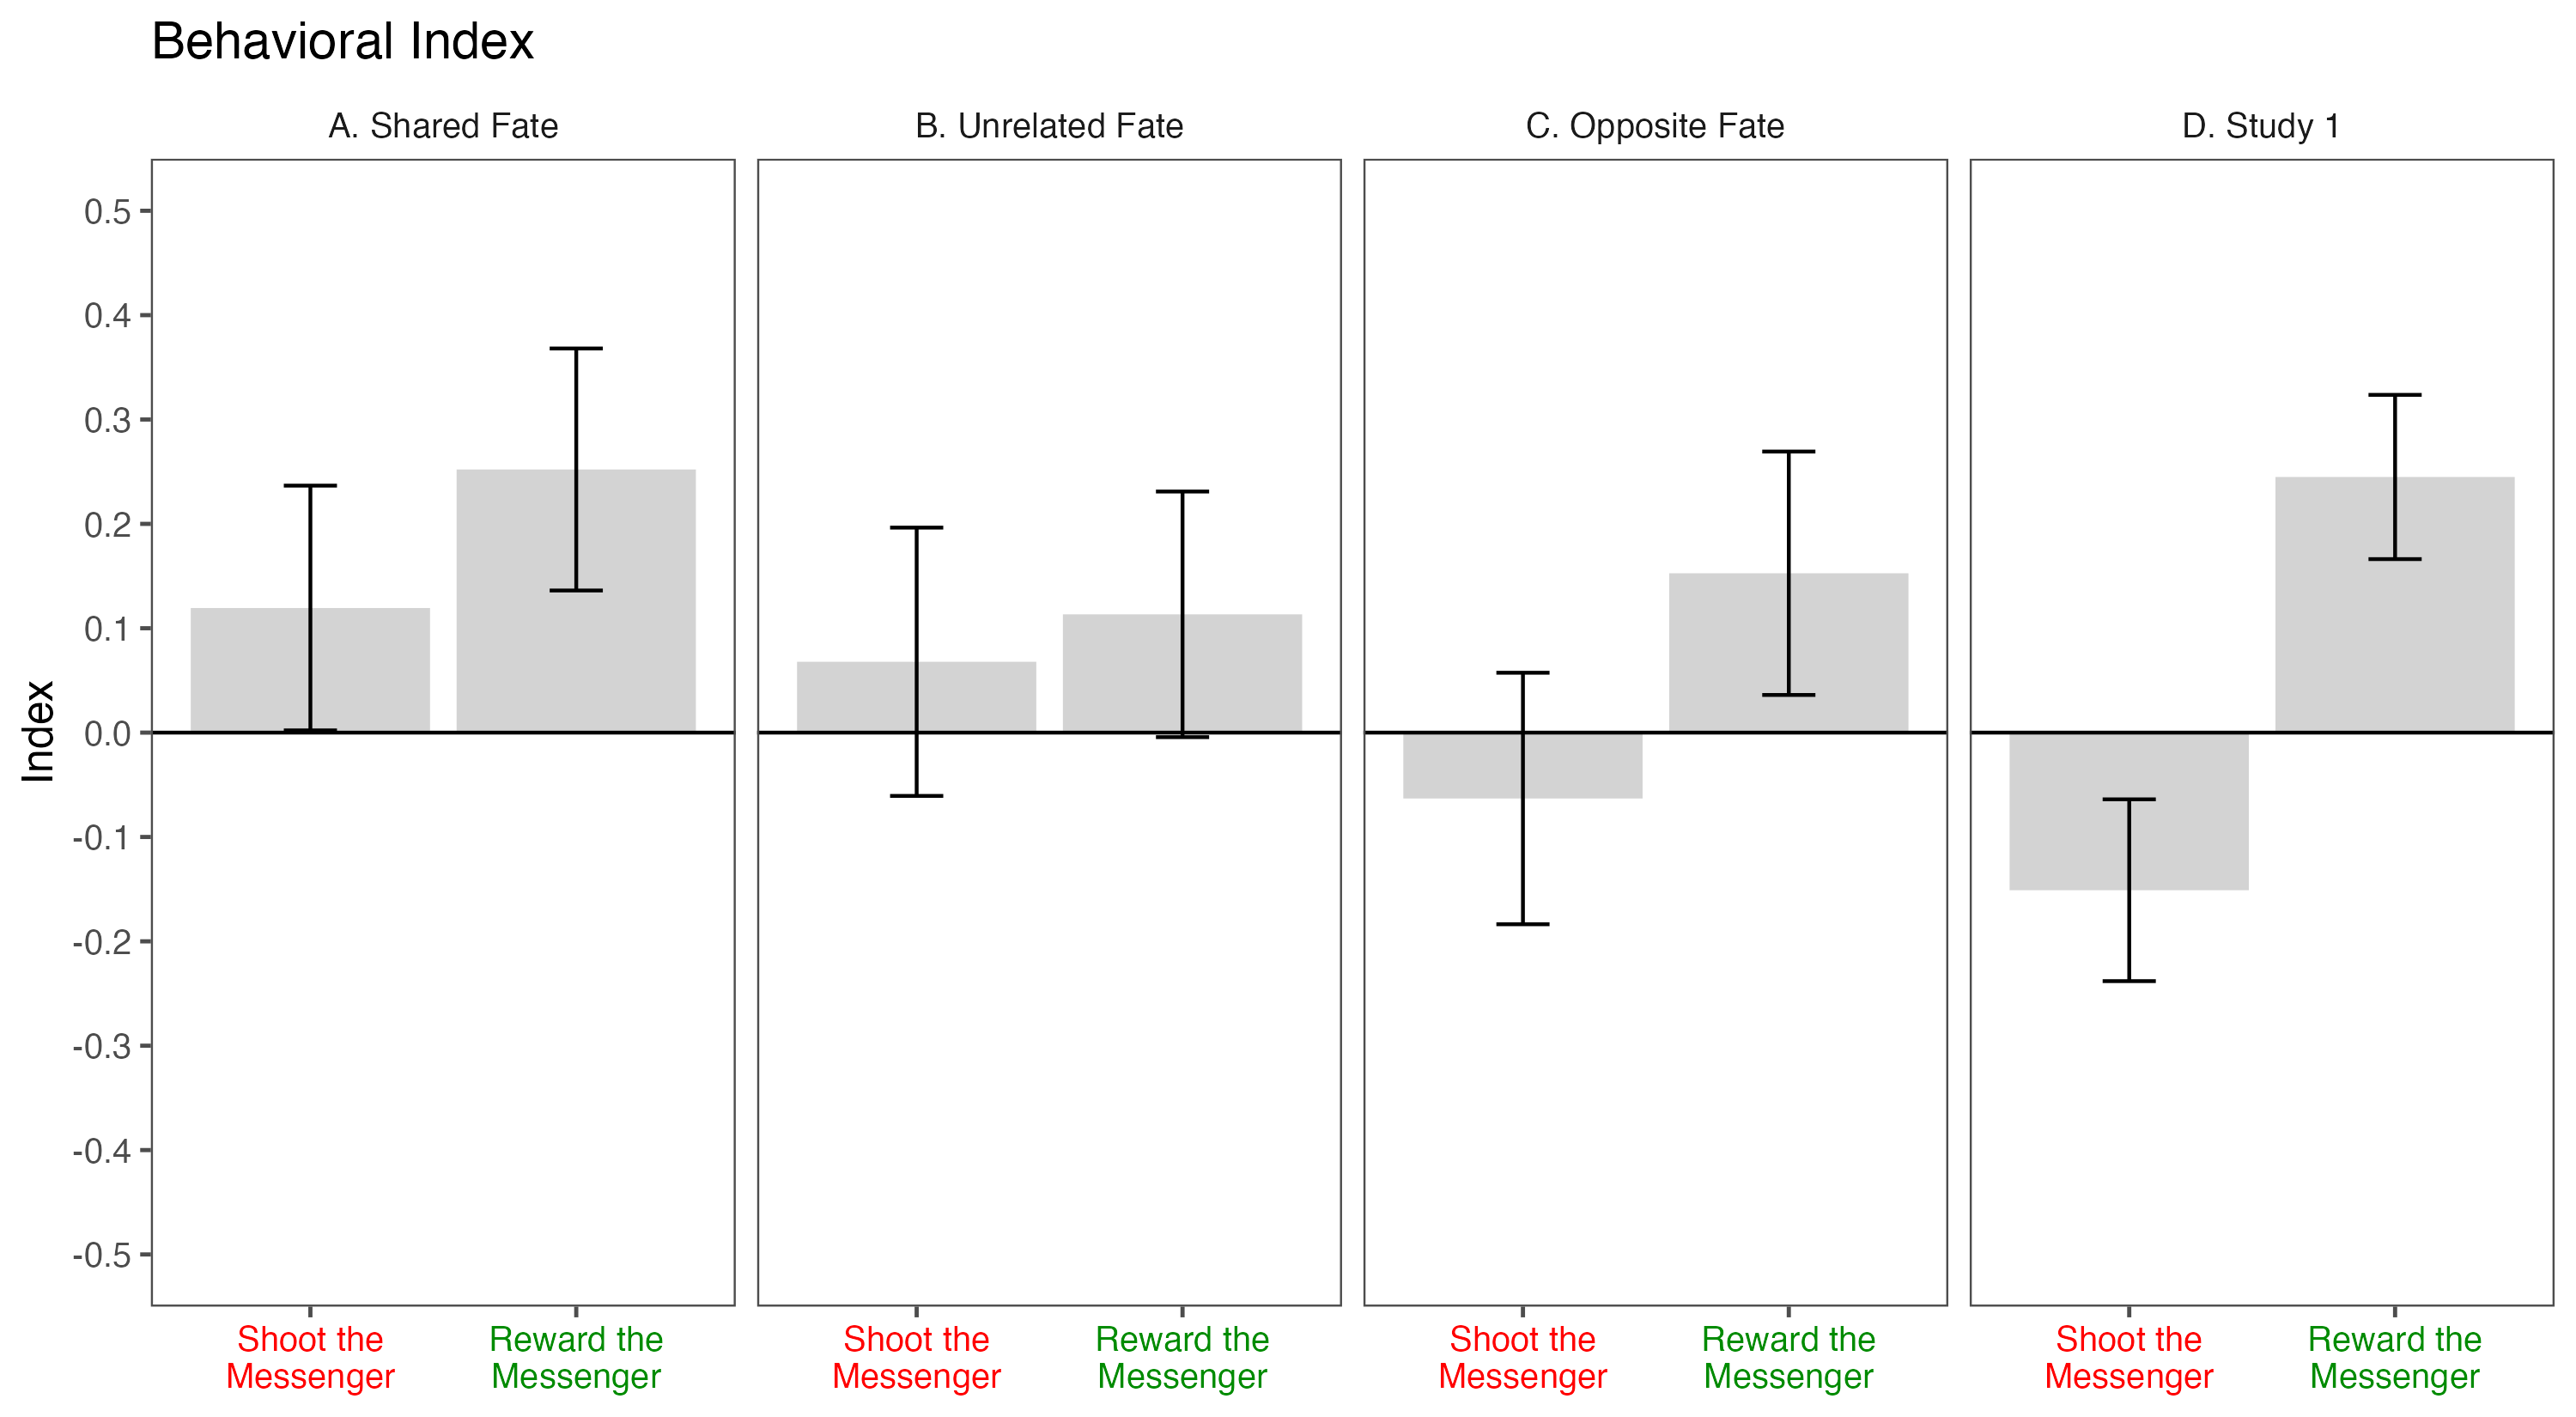
\includegraphics[width=1.0\textwidth]{figures/study2_main_behavior_all.png}
  \caption{Difference in messenger and non-messenger ratings of the Behavioral Index by losing (STM) and winning (RTM) across Unrelated Fate, Shared Fate, Opposite Fate conditions, Study 2. 
  \textit{Note: OLS regression with robust standard errors, with error bars representing 95\% confidence intervals.In the behavioral index, the DV is calculated by averaging the standardized scores of the dictator game, spin the wheel task, and prisoner's dilemma. The Shared Fate (Panel A), Unrelated Fate (Panel B), and Opposite Fate (Panel C) conditions are when the partner wins when the respondent wins, the partner winning are unrelated to the respondent winning, and the partner wins when the respondent loses, respectively. Study 1 (Panel D) repeats the index measure from Study 1 as a reference, where respondents were not explicitly given the alignment of their partner. The p-values of the test that $RTM = -STM$ are 0.00, 0.04, 0.29, and 0.12, respectively, for the Shared, Unrelated, Opposite Fate conditions, and Study 1. The p-values of the messenger bias are 0.00, 0.1, 0.02, and 0.00, respectively, for the Shared, Unrelated, Opposite Fate conditions, and Study 1.}}
  \label{fig:study2_main_behavior_all}
\end{figure}%
\renewcommand{\baselinestretch}{1.67}%


First, we analyze the effect of winning (reward the messenger) and
losing (shoot the messenger) on the behavioral index in Figure \ref{fig:study2_main_behavior_all}, which allows us to
test whether these conditions eliminate the messenger bias. Across all
three conditions (and similarly to Study 1), we find that the
reward the messenger (RTM) effect remains, although it is not
significant in the unrelated fate condition ($p = .06$). However, we
see that the shoot the messenger (STM) effect is eliminated entirely in
the shared and unrelated fate conditions and attenuated substantially in
the opposite fate condition. In the unrelated fate condition, the STM
effect is positive but not significantly different than 0, although it
is negative but not significant in the opposite fate condition (about
33\% of the estimated effect from Study 1). Finally, the shared
fate condition reverses the STM effect completely---telling the
respondents that the messenger shares their positive or negative outcome
causes respondents to behave in a prosocial manner towards the
messenger, regardless of whether they win or lose. Thus, when comparing
the relative magnitude of the RTM and STM effects, we find that the RTM
effect is significantly larger than the STM effect in the shared and unrelated fate conditions.
Overall, we find evidence that the messenger bias disappears completely
only in the unrelated fate condition, which shows that specifying that
the messenger's outcomes are not related to the respondent's is
effective in getting rid of either positive or negative bias towards the
messenger.

\renewcommand{\baselinestretch}{1.25}%
\begin{figure}[!t]%
  \centering
  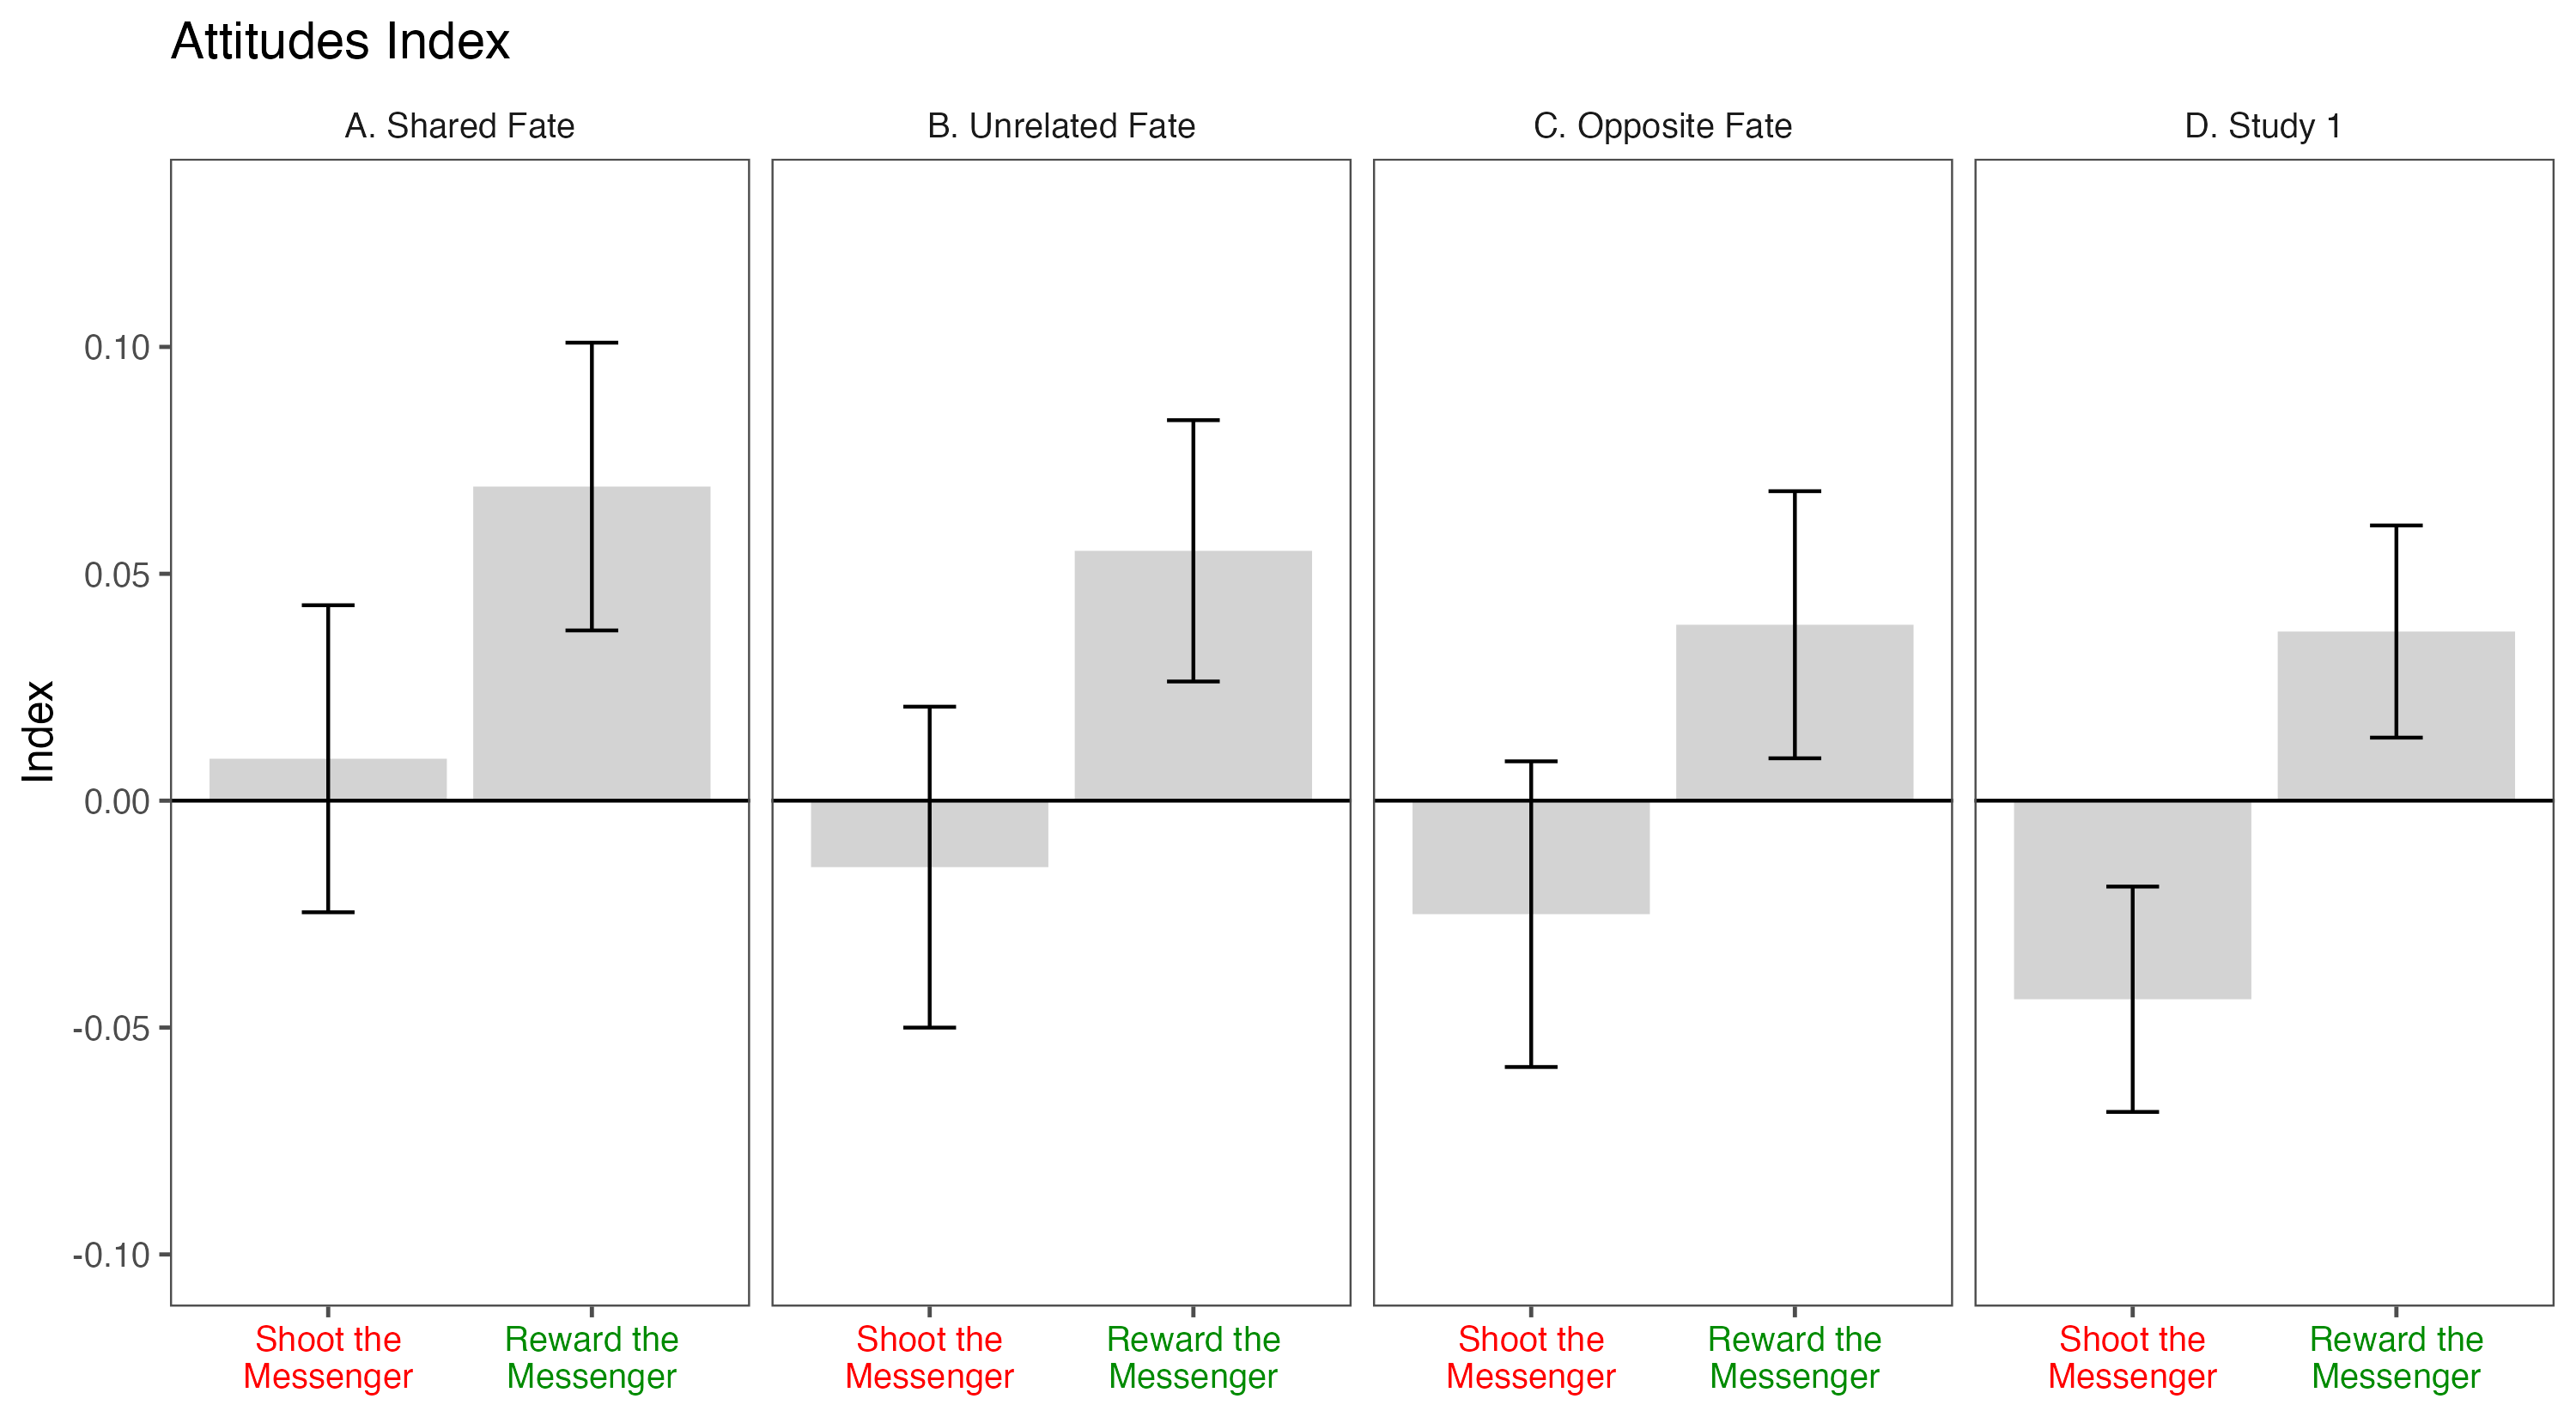
\includegraphics[width=1.0\textwidth]{figures/study2_main_attitude_all.png}
  \caption{Difference in messenger and non-messenger ratings of the Attitudes Index by losing (STM) and winning (RTM) across Unrelated Fate, Shared Fate, Opposite Fate conditions, Study 2. 
  \textit{Note: OLS regression with robust standard errors, with error bars representing 95\% confidence intervals.In the attitudes index, the DV is calculated by averaging the ratings of the trustworthy, nice, likeable, and generous DVs to an index ranging from 0 to 1. The Shared Fate (Panel A), Unrelated Fate (Panel B), and Opposite Fate (Panel C) conditions are when the partner wins when the respondent wins, the partner winning are unrelated to the respondent winning, and the partner wins when the respondent loses, respectively. Study 1 (Panel D) repeats the index measure from Study 1 as a reference, where respondents were not explicitly given the alignment of their partner. The p-values of the test that $RTM = -STM$ are 0.00, 0.08, 0.55, and 0.71, respectively, for the Shared, Unrelated, Opposite Fate conditions, and Study 1. The p-values of the messenger bias are 0.00, 0.00, 0.01, and 0.00, respectively, for the Shared, Unrelated, Opposite Fate conditions, and Study 1.}}
  \label{fig:study2_main_attitude_all}
\end{figure}%
\renewcommand{\baselinestretch}{1.67}%


Next, we analyze the attitudes index in Figure \ref{fig:study2_main_attitude_all}. As with the behavioral index, we
see that the RTM effect persists across all three conditions, although
it is lowest in the opposite fate condition and highest in the shared
fate condition. We also see that the STM effect is not statistically
significant in any condition, although it also monotonically decreases
from the opposite to the shared fate conditions. The point estimate is
positive only in the shared fate condition. As with the behavioral
index, the RTM effects are again significantly larger than the STM
effects in the shared and unrelated fate conditions. However, no condition eliminated the
messenger bias for the attitudinal measures, which implies that
respondents were much more likely to view messengers positively when
they delivered good rather than bad news.

Overall, in Study 2, we find three important results. First, we continue
to find that the STM and RTM effects for behaviors are different than
those for attitudes, even when we specify the fate of the messenger.
Although it may be possible to eliminate the messenger bias for
behaviors, we find no such result for attitudinal measures. Second,
whether the incentives of messenger and respondent are aligned or
misaligned is crucial for determining whether messenger bias arises.
Across all conditions and measures, specifying the stakes of the
messenger in the outcome reversed the sign of or attenuated the STM
effect. In contrast, the RTM effect was present across most conditions
for both behaviors and attitudes. The only exception was the unrelated
fate condition, which was the only treatment to eliminate the messenger
bias completely
for behavioral measures, as we find no STM or RTM effects. Surprisingly,
the shared fate condition induced respondents to reward the messenger regardless of whether
the respondent won or lost: clarifying that the messenger had the same
stakes as the participant elicited more positive behaviors towards
messengers even after losing. Finally, RTM effects were asymmetric to
STM effects. RTM effects are especially persistent across most treatment
conditions and larger than STM effects, which is further evidence from
Study 1 that the RTM and STM effects are not symmetric and deserve to
be examined in turn. We expected the shared (opposite) fate condition to
eliminate (exacerbate) the STM effect and exacerbate (eliminate) the RTM
effect. While we do find this for the shared fate condition, we do not for the opposite fate condition: the STM effect reverses sign in some
conditions, but is still attenuated in the opposite fate condition. In contrast, RTM
effects are persistent across most conditions, even when the messenger has the
opposite incentives of the respondent. This finding points to a fruitful avenue for additional research: What incentives do respondents assume a messenger has when they are not specified?

\section{Discussion}

Across two incentivized experiments with thousands of participants, we
find consistent evidence of the messenger bias and how to mitigate it.
In Study 1, participants both shot and rewarded the messenger for
delivering bad news and good news, respectively. In Study 2, the
STM effect was either eliminated entirely or substantially diminished
across all conditions for both attitudes and behavioral measures when
clarifying the stakes the messenger had in the outcome. Specifically,
when the messenger clarified their (non-)stakes in the outcome
(unrelated fate), participants did not dislike the messenger more and
did not treat the messenger better or worse than a non-messenger. In the
shared and opposite fate conditions, the RTM effect persisted for both
attitudinal and behavioral measures. When incentives were aligned
(shared fate conditions), both the RTM and STM effects were positive, as
respondents behaved more prosocially regardless of whether they won or
lost. When incentives were misaligned (opposite fate conditions),
participants still consistently rewarded messengers delivering good
news but failed to punish messengers for delivering bad news.

Our paper contributes three new findings to the literature. First, we go
beyond the prior exclusive focus on the STM effect and look at both the
STM and RTM effects together. The STM effect may be a major source of
inefficiency in society because messengers know that backlash may await
them after communicating bad news. Moreover, in an environment where
messengers know that they face punishment for breaking bad news and
rewards for conveying good news, messengers have incentives to alter or
withdraw news. Thus, information cannot be easily trusted, possibly
breeding inefficiencies and a decline in cooperation in the absence of
strategies or institutions that restore incentives for messengers to
tell the truth. However, we also find that the RTM effect is greater
than or equal to the STM effect and surprisingly resilient in Study 2
compared to the STM effect. The RTM effect is just as normatively concerning
and deserving attention because it suggests people may rush to convey
good news regardless of whether they contributed to the good outcome. At
one extreme, people's intuitions to reward pure messengers may skew the
incentives in the communication environment from producing good news to
communicating it. This may be undesirable because it puts the creators
of good outcomes for society at a relative disadvantage compared to the
people who communicate those outcomes to the public, such as influencers
on social media or spokespersons.

Second, the present experiments provide the first evidence of a
messenger bias that affects prosocial behavior and goes beyond
attitudes. When no information about the messenger's payoffs was
provided in Study 1, respondents' attitudes toward the messenger
indicated that they rate the messenger to be less trustworthy, nice,
likeable, and generous after losing and the opposite after winning. Yet,
behavioral measures show that this does not extend to acting less
trusting after losing (shooting the messenger for spin the wheel) or
more cooperative after winning (rewarding the messenger for prisoner's
dilemma). Study 2 confirms this discrepancy between behavioral and
attitudinal measures, as the unrelated fate condition was able to
eliminate the messenger bias completely for behavioral measures, but the
messenger bias persisted for attitudinal measures across all conditions.
Therefore, only focusing on attitudinal measures like prior work would
overestimate the impact of the messenger bias, as biased attitudes may
not translate into biased behaviors towards the messenger. This study
demonstrates the importance of using behavioral measures to better
understand the implications of the messenger bias and how to reduce it.

Finally, we show one effective strategy that broadly eliminates STM
effects for biased behaviors: specifying the incentives of the messenger
in the message outcome. Our second experiment was effective in broadly
reducing the STM effect for cooperation, altruism, and trust toward
messengers, along with attitudinal measures. Yet, a limitation of our
current research is that we only somewhat ameliorated the RTM effect (for the unrelated fate condition for behaviors), and even
exacerbated it with the shared fate conditions. This may still be
problematic as individuals were rewarded for mechanically announcing
good news which they did not create. While we identify one potential
strategy to ameliorate the RTM and STM effects, future research should
explore other effective strategies beyond clarifying the relationship
between the messenger and the message. These could involve avoiding using
controlling or abstract messages \citep[see, e.g.,][]{sparks2008style,miller2007psychological} or increasing messenger credibility \citep[see, e.g.,][]{hunt1984role,kamins1987twosided}. 
Future work can then
continue to unravel the messenger bias and its impact on interpersonal
relations, markets, and politics, along with how to mitigate these
impacts.


\section{Methods}

\subsection{Study 1 Methods}

We recruited 2,762 participants from the United States on MTurk
\citep{berinsky2012evaluating}. 763 participants failed our preregistered
screeners (appendix), yielding a final sample of 1,999 subjects (61\%
female; age: \emph{M} = 41, \emph{SD} = 13 years) (see Table \ref{tab:exp1_sample} for more sample demographics). 
Participants read the
experimental instructions, answered comprehension questions, and
proceeded to the experiment. After the survey, participants were matched
with their partners and compensated based on the outcomes of tasks 1 and
2 as well as their performance in the quiz questions before each task.
The bonus was in addition to a flat fee for participating (70 cents).

\subsubsection{Design}

The experiment involved two parts. In the first part, treatment was
administered, as respondents were matched to a partner, a messenger, who
observed their performance in a task and communicated the result to
them. In the second part, participants played a dictator game, a
spin-the-wheel task, and a prisoner's dilemma game. In the first part,
participants were assigned to either a \emph{number counting task} or a
\emph{prediction task}. Specifically, they earned a bonus of 50 cents
for correctly identifying which of two 6 x 6 grids contained more odd
numbers in 20 seconds or for correctly predicting the outcome of a coin
toss. The number counting task was designed to give the impression that
the outcome is influenced by skill, whereas the prediction task aimed to
convey the idea that the outcome was the result of pure luck. However,
as intended, we did not find any statistical difference between the
outcomes of the counting and prediction tasks (other than the RTM effect for the prisoner's dilemma), 
meaning that empirically,
the counting task was equivalent to a coin toss. After the task,
participants received the news about the outcome from their partner
(``the messenger''). The messenger used either neutral language (``Your
count was correct/incorrect'' or ``Your coin toss prediction matched/did
not match the coin toss'') or emotional language (``Too bad! You lost!''
or ``Congratulations! You won!''). Then, participants read the
instructions for the second part of the experiment and took a
comprehension quiz.

After learning the outcome of the first part, subjects proceeded to the
second part. In the second part, respondents played three games with their
partner who was were randomly assigned to be either the messenger or a
new MTurk participant who was not the messenger. Specifically,
participants played a dictator game, a spin-the-wheel task, and a
prisoner's dilemma game in randomized order. They could earn
up to an extra 50 cents for each game depending on their own decisions
as well as the other player's. The dictator game split the total reward
between the respondent and the respondent. In the spin-the-wheel task,
they chose whether to have the computer or their partner (either the
messenger or a different MTurk participant) spin the wheel on their
behalf. Finally, the prisoner's dilemma was an up or down vote to
cooperate with the messenger or not.

In sum, participants were evenly assigned to one of eight conditions.
Specifically, we used a 2 (luck: prediction task vs. skill: number
counting task) x 2 (emotional language vs. neutral language) x 2
(messenger vs. another participant who is not the messenger)
between-subjects design.

Additionally, we randomly assigned one-third of the sample to answer
attitudes questions about the messenger just after the first task. The
remaining two-thirds of the sample was evenly split between participants
who answered the attitudes questions about the messenger or the partner
depending on whether they were paired with the messenger or the partner
in the three behavioral games. These questions were asked after the
games.

\subsubsection{Measures}

Our main pre-registered outcome measures are behavioral: participants'
decisions in the dictator game, spin-the-wheel task, and prisoner's
dilemma game. We analyzed participants' decisions in the games
separately, since each game aims to measure a different construct. The
dictator game measures altruism \citep{bekkers2007measuring, benenson2007children,johannesson2000non}, 
the spin-the-wheel task captures a
possible halo effect of the messenger, and the prisoner's dilemma is a
proxy for cooperation \citep{bendor1991doubt, rapoport1965prisoner}.\footnote{While 
we do not pre-register a combined index for the
  behavioral outcomes in Study 1 like we did in Study 2, we
  also created and analyzed a behavioral index variable combining these
  behavioral outcomes to be able to compare Studies 1 and 2.}

Additionally, we included attitudinal measures about the messenger and
non-messenger. To measure attitudes toward the messenger or the
non-messenger, participants rated their trustworthiness, niceness,
likeability, and generosity on a 7-point scale ranging from ``Not at
all'' to ``Extremely.'' The combined scale about attitudes toward the
messenger (analyses in the Appendix) (attitudes asked first: $\alpha =
0.91$; attitudes asked after: $\alpha = 0.95$) and the non-messenger were
reliable ($\alpha = 0.89$).\footnote{For the attitudes index variable, which combines these three scales,
we conduct principal component analysis on the four attitudes measures 
and find a sharp drop-off from the eigenvalue of the first dimension
to the second, thus validating our choice to use a single index.} At the end of the survey, participants had the
opportunity to provide open-ended comments.

\subsubsection{Research Design}

\begin{table}[]
\centering
\caption{Simplified research design of winning or losing compared to the messenger or non-messenger}
\label{tab:research-design}
\begin{threeparttable}
\begin{tabular}{@{}lcc@{}}
\toprule
\textbf{} & \multicolumn{1}{l}{\textbf{1st Round Win}} & \multicolumn{1}{l}{\textbf{1st Round Loss}} \\ \midrule
\textbf{Messenger} & A & B \\
\textbf{Non-messenger} & C & D \\ \bottomrule
\end{tabular}%
\begin{tablenotes}[flushleft]
\scriptsize{\item[\hspace{-5mm}] \textit{Note:} The columns represent whether the respondent received a message that said that they won or lost. The rows represent instances in which the respondent then plays a game with the messenger or non-messenger.}
\end{tablenotes}
\end{threeparttable}
\end{table}

For Study 1, we first look at a simplified research design that only
focuses on our main experimental conditions in Table \ref{tab:research-design} to determine the
quantities of interest. For each of the dependent variables (dictator
game, spin the wheel, prisoner's dilemma, behavioral index, trustworthy,
nice, likeable, generous, attitudes index), we calculate the same four
quantities of interest. First, the reward the messenger effect is
calculated by $A-C$, which asks whether the messenger gets rewarded
for delivering good news. Our prior hypothesis is that this RTM effect
is greater than 0. Second, the shoot the messenger effect is calculated
by $B-D$, which asks whether the messenger gets punished for
delivering bad news. Our prior hypothesis is that this STM effect is
less than 0. Finally, the total messenger bias (TMB), which asks whether
the subjects' behavior towards the messenger depends on delivering a
winning or losing message, is determined by whether both the STM and RTM
effect exists, which is calculated by $A-C = 0$ and $B-D =
0$.\footnote{As noted above, \citet{john2019shooting}'s analysis of the STM effect
 only looks at $A-B$, which may conflate the valence effect
  of receiving a bad news from actually shooting the messenger for
  delivering bad news. We avoid this with the inclusion of the
  non-messenger conditions when we measure the shoot the messenger
  effect.}

For the rest of our analyses, we use OLS linear regression to formally
analyze respondents' decisions. In each of the behavioral and attitudinal
outcomes, we model each outcome using linear regression with robust
standard errors and indicators for randomly assigned treatment
conditions.\footnote{As a robustness check, we also consider
more complex regression models for the behavioral measures. 
When we conduct generalized linear regressions (tobit regression with censoring at 0 and 50 cents for the dictator game variable, 
and logistic regression for the spin the wheel and prisoner’s dilemma variables)
in Tables \ref{tab:behavior_logit_regression}, 
\ref{tab:behavior_logit_regression_emotional}, and \ref{tab:behavior_logit_regression_counting}, following 
the logic of the main results, 
we do not find that substantive results vary from the OLS regressions for the behavioral measures.} 
That is, we specify:\footnote{To test whether the emotionality of the message or the type of task matters,
we interact the following regression with indicator variables for whether the respondent received an
emotional message and whether the respondent performed the counting task in Tables \ref{tab:behavior_regression_emotional}
and \ref{tab:behavior_regression_counting}, respectively. The latter regression is a deviation from our
pre-registered analysis from Study 1, in which we stated that we would examine the effect of the counting task
by interacting the 
type of task with the messenger instead.}

\[{Outcome}_{i} = \beta_{0} + \beta_{1}*Lost  + \beta_{2}*Messenger + \beta_{3}*Lost*Messenger + \varepsilon\]

Therefore, $H_0\colon \beta_2$ is an estimate of the effect
of rewarding the messenger, or RTM, (compared to rewarding the
non-messenger, the excluded category) while winning. Alternatively,
$H_o\colon \beta_2 + \beta_3$ is the estimate of the
effect of shooting the messenger, or STM, (compared to shooting the
non-messenger, the excluded category) while losing. We also investigate the relative magnitudes of rewarding and shooting the messenger, which
means we are testing whether the $RTM = -STM$ (since we expect the shoot
the messenger effect to be negative), which is a linear combination of
parameters test of $\beta_2 = -\beta_2 -
\beta_3$, which is equivalent to testing
$2\beta_2 + \beta_3 = 0$. Finally, the last quantity of interest is total
messenger bias (TMB), for which we conduct a joint hypothesis test that the RTM
and STM are simultaneously equal to 0, which is $H_0\colon \beta_2,
\beta_3 = 0$. 

\subsection{Study 2 Methods}

We recruited 3,576 participants from the United States on MTurk
\citep{berinsky2012evaluating}. 567 participants failed the initial screeners
and were excluded from proceeding further in the experiment, yielding a
final sample of 3,000 participants (60\% female; age: \emph{M} = 41,
\emph{SD} = 13 years) (see Table \ref{tab:exp2_sample} for more demographics). 
The flow of the experiment was the same as in
Study 1. After the survey, participants were matched and compensated
following the same procedure as used in Study 1. The bonus was in
addition to a flat fee for participating (70 cents). As in Study 1, we
recruited 99 messengers to ensure that participants' choices produced
real financial consequences for human messengers.

\subsubsection{Design}

The design was identical to Study 1 except in two respects. First, we
did not include emotional messages and the attitudes questions were
asked only after the behavioral games. Second, and more substantively,
we manipulated whether the messenger's fate was unrelated to the
participant, shared with the participant, or opposite of the
participant. Specifically, in the unrelated fate condition, the
messenger did not earn any additional money regardless of the outcome of
task 1. This was communicated in the message announcing the outcome,
where the messenger specified that they did not earn any money for
delivering the message. In contrast, when the messenger shared the same
fate as the participant, if a participant won 50 cents, the messenger
earned 5 cents or 50 cents depending on the condition. If a participant
lost and did not earn any money, the messenger did not earn any money
either. Similarly, in the opposite fate conditions, the messenger did
not earn any money when the participant won whereas they earned 5 or 50
cents depending on the condition when the participant lost in task 1. 
The messenger always announced their own earnings when they communicated
the outcome of task 1. In sum, in Study 2, we used a 2 (task 1:
prediction vs. count) x 2 (partner: messenger vs. another participant) x
5 (fate: unrelated vs. shared 5 vs. shared 50 vs. opposite 5 vs.
opposite 50) between-subjects design.

\subsubsection{Measures}

Our main outcome measures are the same as in Study 1, except that here
we preregistered that we would analyze the behavioral games as an index
of behavioral prosociality. The behavioral index is constructed as the
average of the standardized scores for the three behavioral games across
the entire sample. Each standardized score has \emph{M} = 0 and
\emph{SD} = 1. Thus, the resulting behavioral index has \emph{M} = 0,
\emph{SD} = 0.69, and ranges between $-1.3$ and $+1.3$, where a higher score
indicates more prosociality. The attitudes scale, which ranges from 1
(negative attitudes) to 7 (positive attitudes), had excellent
reliability ($\alpha = 0.94$). We pooled together the shared 5 and shared
50 cent fate conditions into one shared fate condition. 
Similarly, for the opposite 5 and 50 cent fate conditions, 
where the messenger earned money (5 or 50 cents
depending on the condition) when the participant lost and did not earn
any money when the participant won, we also pool these into one opposite fate 
condition.\footnote{In Figures
\ref{fig:study2_main_fivecent_behavior_all} and \ref{fig:study2_main_fivecent_attitude_all}, 
we break out each of the shared and
unrelated fate conditions to instances in which the partner received a 5 cent or
50 cent bonus. For the shared fate conditions, there are no differences between
the messenger winning or losing 50 cents or 5 cents for the RTM and STM effects
for both behaviors and attitudes (see Panels A and B). We see slight differences in the 
RTM effect between the 5 and 50 cent opposite fate conditions for both behaviors and attitudes. 
While the respondent continues to reward the messenger in the 5 cent opposite fate condition (Panel D), 
the RTM effect is not significant in the 50 cent opposite fate condition, in which
 the messenger wins 50 cents when the respondent
loses (Panel E).}

\subsubsection{Research Design}
In Study 2, we conduct the exact same analysis as Study 1, but focus on only the pooled
dependent variable (behavioral and attitudes index) for simplicity. We
analyze each of the alignment conditions (shared, unrelated, and
opposite fate) separately to see how the reward the messenger and shoot
the messenger effects shift when we specify the alignment of the
messenger.

%% REFERENCES ------------------------------------------------------------------------
\clearpage{}
\setstretch{1.5}

%\bibliographystyle{bibfiles/apsa-leeper}
\bibliographystyle{apsr}
\bibliography{bibfiles/stm.bib}

%% SUPPLEMENTARY MATERIALS -----------------------------------------------------------
\clearpage
\appendix
\thispagestyle{empty}

\doparttoc % Tell to minitoc to generate a toc for the parts
\faketableofcontents % Run a fake tableofcontents command for the partocs

\begin{center}
{\bf \LARGE Supplementary Materials} \\
\vspace{0.2in}
{\doublespacing\Large \tit}
\end{center}

\addcontentsline{toc}{section}{Appendix} % Add the appendix text to the document TOC
\part{} % Start the appendix part
\parttoc % Insert the appendix TOC
\setstretch{1}

\clearpage
\renewcommand{\thepage}{A\arabic{page}}
\counterwithin{table}{section}
\counterwithin{figure}{section}
\setcounter{section}{0}
\setcounter{page}{1}
\setcounter{table}{0}
\setcounter{footnote}{0}
\renewcommand{\thetable}{\Alph{section}\arabic{table}}
\renewcommand{\thefigure}{\Alph{section}\arabic{figure}}
\renewcommand{\baselinestretch}{1.25}
\setlength{\footnotesep}{1.25 \footnotesep}


\section{Study 1 Results}
\label{sec:appendix_study1}

\subsection{Main Results}
\renewcommand{\baselinestretch}{1.25}%

\begin{table}[!ht]
\caption{Regressions of behavioral measures on losing in task 1, being paired with the messenger, and their interaction}
\begin{center}
\scalebox{1}{
\begin{threeparttable}
\begin{tabular}{l c c c c}
\toprule
 & \makecell{Dictator\\Game} & \makecell{Spin the\\Wheel} & \makecell{Prisoner's\\Dilemma} & \makecell{Behavioral\\Index} \\
\midrule
Lost T1                                          & $-0.446$       & $-0.005$       & $0.020$        & $-0.000$       \\
                                                 & $(0.827)$      & $(0.032)$      & $(0.027)$      & $(0.041)$      \\
Messenger                                        & $2.488^{**}$   & $0.221^{***}$  & $0.044$        & $0.245^{***}$  \\
                                                 & $(0.796)$      & $(0.030)$      & $(0.026)$      & $(0.040)$      \\
Lost x Messenger                                 & $-4.400^{***}$ & $-0.260^{***}$ & $-0.143^{***}$ & $-0.396^{***}$ \\
                                                 & $(1.158)$      & $(0.044)$      & $(0.039)$      & $(0.060)$      \\
Constant                                         & $15.814^{***}$ & $0.475^{***}$  & $0.750^{***}$  & $-0.030$       \\
                                                 & $(0.578)$      & $(0.022)$      & $(0.019)$      & $(0.029)$      \\
\midrule
STM: $\beta_2 + \beta_3 = 0$ $p$-values          & $0.023$        & $0.230$        & $0.001$        & $0.001$        \\
RTM: $\beta_2 = 0$ $p$-values                    & $0.002$        & $0.000$        & $0.091$        & $0.000$        \\
RTM = $-$STM: $2 \beta_2+\beta_3 = 0$ $p$-values & $0.619$        & $0.000$        & $0.155$        & $0.116$        \\
TMB: $\beta_2 = 0, \beta_3 = 0$ $p$-values       & $0.001$        & $0.000$        & $0.001$        & $0.000$        \\
R$^2$                                            & $0.018$        & $0.045$        & $0.011$        & $0.044$        \\
Observations                                     & $1994$         & $1994$         & $1994$         & $1994$         \\
\bottomrule
\end{tabular}
\begin{tablenotes}[flushleft]
\scriptsize{\item[\hspace{-5mm}] \textit{Note:} OLS regressions with robust standard errors in parentheses. 
                                In the dictator game, the dependent variable (DV) is giving up to 50 cents to the partner. 
                                In the spin the wheel task, the DV is choosing the partner to spin the wheel on one’s behalf instead of the computer. 
                                In the prisoner’s dilemma, the DV is choosing cooperation. 
                                In the behavioral index, the DV is calculated by averaging the standardized scores of the dictator game, spin the wheel task, and prisoner's dilemma. \item[\hspace{-5mm}] $^{***}p<0.001$; $^{**}p<0.01$; $^{*}p<0.05$.}
\end{tablenotes}
\end{threeparttable}
}
\label{tab:behavior_regression}
\end{center}
\end{table}

\renewcommand{\baselinestretch}{1.67}%


\renewcommand{\baselinestretch}{1.25}%

\begin{table}[!t]
\caption{Regressions of behavioral measures on losing in task 1, being paired with the messenger, emotionality of message, and their interaction}
\begin{center}
\scalebox{1}{
\begin{threeparttable}
\begin{tabular}{l c c c c}
\toprule
 & \makecell{Dictator\\Game} & \makecell{Spin the\\Wheel} & \makecell{Prisoner's\\Dilemma} & \makecell{Behavioral\\Index} \\
\midrule
Lost T1                      & $-0.424$       & $-0.028$      & $0.054$        & $0.012$        \\
                             & $(1.146)$      & $(0.045)$     & $(0.038)$      & $(0.056)$      \\
Messenger                    & $3.202^{**}$   & $0.204^{***}$ & $0.057$        & $0.262^{***}$  \\
                             & $(1.114)$      & $(0.043)$     & $(0.037)$      & $(0.056)$      \\
Emotional Message            & $0.565$        & $0.013$       & $0.016$        & $0.035$        \\
                             & $(1.158)$      & $(0.044)$     & $(0.038)$      & $(0.058)$      \\
Lost x Messenger             & $-4.306^{**}$  & $-0.199^{**}$ & $-0.188^{***}$ & $-0.387^{***}$ \\
                             & $(1.616)$      & $(0.062)$     & $(0.055)$      & $(0.083)$      \\
Lost x Emotional             & $-0.020$       & $0.047$       & $-0.070$       & $-0.023$       \\
                             & $(1.659)$      & $(0.063)$     & $(0.054)$      & $(0.082)$      \\
Messenger x Emotional        & $-1.402$       & $0.034$       & $-0.026$       & $-0.033$       \\
                             & $(1.591)$      & $(0.060)$     & $(0.052)$      & $(0.080)$      \\
Lost x Messenger x Emotional & $-0.242$       & $-0.124$      & $0.091$        & $-0.019$       \\
                             & $(2.319)$      & $(0.088)$     & $(0.078)$      & $(0.120)$      \\
Constant                     & $15.528^{***}$ & $0.468^{***}$ & $0.742^{***}$  & $-0.047$       \\
                             & $(0.836)$      & $(0.031)$     & $(0.028)$      & $(0.041)$      \\
\midrule
R$^2$                        & $0.019$        & $0.047$       & $0.012$        & $0.045$        \\
Observations                 & $1994$         & $1994$        & $1994$         & $1994$         \\
\bottomrule
\end{tabular}
\begin{tablenotes}[flushleft]
\scriptsize{\item[\hspace{-5mm}] \textit{Note:} OLS regressions with robust standard errors in parentheses. 
                                In the dictator game, the dependent variable (DV) is giving up to 50 cents to the partner. 
                                In the spin the wheel task, the DV is choosing the partner to spin the wheel on one’s behalf instead of the computer. 
                                In the prisoner’s dilemma, the DV is choosing cooperation. 
                                In the behavioral index, the DV is calculated by averaging the standardized scores of the dictator game, spin the wheel task, and prisoner's dilemma. \item[\hspace{-5mm}] $^{***}p<0.001$; $^{**}p<0.01$; $^{*}p<0.05$.}
\end{tablenotes}
\end{threeparttable}
}
\label{tab:behavior_regression_emotional}
\end{center}
\end{table}

\renewcommand{\baselinestretch}{1.67}%


\renewcommand{\baselinestretch}{1.25}%

\begin{table}[!t]
\caption{Regressions of behavioral measures on losing in task 1, being paired with the messenger, type of task, and their interaction}
\begin{center}
\scalebox{1}{
\begin{threeparttable}
\begin{tabular}{l c c c c}
\toprule
 & \makecell{Dictator\\Game} & \makecell{Spin the\\Wheel} & \makecell{Prisoner's\\Dilemma} & \makecell{Behavioral\\Index} \\
\midrule
Lost T1                     & $-0.256$       & $0.009$        & $0.039$       & $0.029$        \\
                            & $(1.172)$      & $(0.044)$      & $(0.039)$     & $(0.059)$      \\
Messenger                   & $3.472^{**}$   & $0.237^{***}$  & $0.109^{**}$  & $0.330^{***}$  \\
                            & $(1.162)$      & $(0.043)$      & $(0.037)$     & $(0.057)$      \\
Counting Task               & $1.016$        & $0.092^{*}$    & $0.070$       & $0.141^{*}$    \\
                            & $(1.161)$      & $(0.044)$      & $(0.038)$     & $(0.058)$      \\
Lost x Messenger            & $-4.894^{**}$  & $-0.257^{***}$ & $-0.179^{**}$ & $-0.434^{***}$ \\
                            & $(1.624)$      & $(0.062)$      & $(0.055)$     & $(0.083)$      \\
Lost x Counting             & $-0.302$       & $-0.021$       & $-0.035$      & $-0.049$       \\
                            & $(1.665)$      & $(0.063)$      & $(0.054)$     & $(0.082)$      \\
Messenger x Counting        & $-1.938$       & $-0.028$       & $-0.128^{*}$  & $-0.167^{*}$   \\
                            & $(1.595)$      & $(0.059)$      & $(0.052)$     & $(0.080)$      \\
Lost x Messenger x Counting & $0.896$        & $-0.011$       & $0.065$       & $0.066$        \\
                            & $(2.326)$      & $(0.088)$      & $(0.078)$     & $(0.120)$      \\
Constant                    & $15.290^{***}$ & $0.427^{***}$  & $0.714^{***}$ & $-0.102^{*}$   \\
                            & $(0.875)$      & $(0.031)$      & $(0.029)$     & $(0.043)$      \\
\midrule
R$^2$                       & $0.019$        & $0.050$        & $0.015$       & $0.048$        \\
Observations                & $1994$         & $1994$         & $1994$        & $1994$         \\
\bottomrule
\end{tabular}
\begin{tablenotes}[flushleft]
\scriptsize{\item[\hspace{-5mm}] \textit{Note:} OLS regressions with robust standard errors in parentheses. 
                                In the dictator game, the dependent variable (DV) is giving up to 50 cents to the partner. 
                                In the spin the wheel task, the DV is choosing the partner to spin the wheel on one’s behalf instead of the computer. 
                                In the prisoner’s dilemma, the DV is choosing cooperation. 
                                In the behavioral index, the DV is calculated by averaging the standardized scores of the dictator game, spin the wheel task, and prisoner's dilemma. \item[\hspace{-5mm}] $^{***}p<0.001$; $^{**}p<0.01$; $^{*}p<0.05$.}
\end{tablenotes}
\end{threeparttable}
}
\label{tab:behavior_regression_counting}
\end{center}
\end{table}

\renewcommand{\baselinestretch}{1.67}%


\renewcommand{\baselinestretch}{1.25}%

\begin{table}[!t]
\caption{Regressions of attitude measures on losing in task 1, being paired with the messenger, and their interaction}
\begin{center}
\scalebox{0.88}{
\begin{threeparttable}
\begin{tabular}{l c c c c c}
\toprule
 & Trustworthy & Nice & Likeable & Generous & \makecell{Attitudes\\Index} \\
\midrule
Lost T1                                         & $-0.310^{***}$ & $-0.480^{***}$ & $-0.461^{***}$ & $-0.532^{***}$ & $-0.075^{***}$ \\
                                                & $(0.088)$      & $(0.079)$      & $(0.078)$      & $(0.082)$      & $(0.012)$      \\
Messenger                                       & $0.253^{**}$   & $0.184^{*}$    & $0.283^{***}$  & $0.182^{*}$    & $0.037^{**}$   \\
                                                & $(0.083)$      & $(0.076)$      & $(0.076)$      & $(0.079)$      & $(0.012)$      \\
Lost x Messenger                                & $-0.472^{***}$ & $-0.440^{***}$ & $-0.566^{***}$ & $-0.479^{***}$ & $-0.081^{***}$ \\
                                                & $(0.123)$      & $(0.111)$      & $(0.111)$      & $(0.118)$      & $(0.017)$      \\
Constant                                        & $4.760^{***}$  & $4.678^{***}$  & $4.678^{***}$  & $4.551^{***}$  & $0.611^{***}$  \\
                                                & $(0.063)$      & $(0.056)$      & $(0.056)$      & $(0.058)$      & $(0.009)$      \\
\midrule
STM: $\beta_2 + \beta_3 = 0$ $p$-values         & $0.016$        & $0.002$        & $0.001$        & $0.001$        & $0.001$        \\
RTM: $\beta_2 = 0$ $p$-values                   & $0.002$        & $0.016$        & $0.000$        & $0.021$        & $0.002$        \\
RTM = $-$STM: $2\beta_2+\beta_3 = 0$ $p$-values & $0.775$        & $0.520$        & $0.995$        & $0.331$        & $0.709$        \\
TMB: $\beta_2 = 0, \beta_3 = 0$ $p$-values      & $0.001$        & $0.000$        & $0.000$        & $0.000$        & $0.000$        \\
R$^2$                                           & $0.045$        & $0.080$        & $0.093$        & $0.087$        & $0.092$        \\
Observations                                    & $1993$         & $1992$         & $1992$         & $1991$         & $1989$         \\
\bottomrule
\end{tabular}
\begin{tablenotes}[flushleft]
\scriptsize{\item[\hspace{-5mm}] \textit{Note:} OLS regressions with robust standard errors in parentheses. 
The trustworthy, nice, likeable, and generous DVs asks respondents to rate these messenger's characteristics on a 7-point Likert scale, where a score of 1 indicates that the messenger does not have that trait at all, while a score of 7 means that a trait describes the messenger extremely well.
    In the attitudes index, the DV is calculated by averaging the standardized ratings of the trustworthy, nice, likeable, and generous DVs to an index ranging from 0 to 1. \item[\hspace{-5mm}] $^{***}p<0.001$; $^{**}p<0.01$; $^{*}p<0.05$.}
\end{tablenotes}
\end{threeparttable}
}
\label{tab:attitude_regression}
\end{center}
\end{table}

\renewcommand{\baselinestretch}{1.67}%


\clearpage
\subsection{Additional Results}

\renewcommand{\baselinestretch}{1.25}%
\begin{table}[H]
\centering

\begin{threeparttable}
\caption{Sample demographics, Experiment 1}

\begin{tabular}[t]{lcccc}
\toprule
Variable & Mean & SD & Min & Max\\
\midrule
Dictator Game Outcome & 15.813 & 13.011 & 0 & 50\\
Spin the Wheel Outcome & 0.522 & 0.500 & 0 & 1\\
Prisoner's Dilemma Outcome & 0.748 & 0.434 & 0 & 1\\
Trustworthiness Outcome & 4.628 & 1.400 & 1 & 7\\
Niceness Outcome & 4.438 & 1.292 & 1 & 7\\
Likeable Outcome & 4.466 & 1.300 & 1 & 7\\
Generous Outcome & 4.275 & 1.366 & 1 & 7\\
Age & 40.848 & 12.978 & 16 & 84\\
Female & 0.610 & 0.488 & 0 & 1\\
Ideology & 2.719 & 1.099 & 1 & 5\\
Education & 4.752 & 1.779 & 1 & 7\\
Employed & 0.721 & 0.448 & 0 & 1\\
White & 0.777 & 0.417 & 0 & 1\\
Hispanic & 0.081 & 0.273 & 0 & 1\\
Belief in Luck Scale & 0.384 & 0.198 & 0 & 1\\
Emotion Regulation Scale & 0.201 & 0.216 & 0 & 1\\
Just World Scale & 0.426 & 0.218 & 0 & 1\\
\bottomrule
\end{tabular}
\label{tab:exp1_sample}
\begin{tablenotes}[flushleft]
\scriptsize
\item[\hspace{-5mm}] 
\end{tablenotes}
\end{threeparttable}
\end{table}
\renewcommand{\baselinestretch}{1.67}%


\renewcommand{\baselinestretch}{1.25}%

\begin{table}[!t]
\caption{Generalized linear regressions of behavioral measures on losing in task 1, being paired with the messenger, and their interaction}
\begin{center}
\scalebox{1}{
\begin{threeparttable}
\begin{tabular}{l c c c}
\toprule
 & \makecell{Dictator\\Game} & \makecell{Spin the\\Wheel} & \makecell{Prisoner's\\Dilemma} \\
\midrule
Lost T1          & $-0.722$       & $-0.022$       & $0.107$        \\
                 & $(1.196)$      & $(0.127)$      & $(0.149)$      \\
Messenger        & $3.442^{**}$   & $0.928^{***}$  & $0.250$        \\
                 & $(1.122)$      & $(0.130)$      & $(0.148)$      \\
Lost x Messenger & $-6.450^{***}$ & $-1.085^{***}$ & $-0.747^{***}$ \\
                 & $(1.691)$      & $(0.184)$      & $(0.208)$      \\
Constant         & $13.083^{***}$ & $-0.102$       & $1.099^{***}$  \\
                 & $(0.845)$      & $(0.089)$      & $(0.102)$      \\
\midrule
Observations     & $1994$         & $1994$         & $1994$         \\
\bottomrule
\end{tabular}
\begin{tablenotes}[flushleft]
\scriptsize{\item[\hspace{-5mm}] \textit{Note:} Tobit regression with robust standard errors in parentheses for the first column (censoring at 0 and 50 cents),
                                and logistic regressions with robust standard errors in parentheses for the second and third column.
                                In the dictator game, the dependent variable (DV) is giving up to 50 cents to the partner. 
                                In the spin the wheel task, the DV is choosing the partner to spin the wheel on one’s behalf instead of the computer. 
                                In the prisoner’s dilemma, the DV is choosing cooperation. \item[\hspace{-5mm}] $^{***}p<0.001$; $^{**}p<0.01$; $^{*}p<0.05$.}
\end{tablenotes}
\end{threeparttable}
}
\label{tab:behavior_logit_regression}
\end{center}
\end{table}

\renewcommand{\baselinestretch}{1.67}%


\renewcommand{\baselinestretch}{1.25}%

\begin{table}[!t]
\caption{Generalized linear regressions of the behavioral measures on losing in task 1, being paired with the messenger, emotionality of message, and their interaction}
\begin{center}
\scalebox{0.9}{
\begin{threeparttable}
\begin{tabular}{l c c c}
\toprule
 & \makecell{Dictator\\Game} & \makecell{Spin the\\Wheel} & \makecell{Prisoner's\\Dilemma} \\
\midrule
Lost T1                      & $-0.637$       & $-0.114$      & $0.305$        \\
                             & $(1.640)$      & $(0.180)$     & $(0.213)$      \\
Messenger                    & $4.298^{**}$   & $0.844^{***}$ & $0.325$        \\
                             & $(1.548)$      & $(0.183)$     & $(0.212)$      \\
Emotional Message            & $0.433$        & $0.050$       & $0.083$        \\
                             & $(1.662)$      & $(0.177)$     & $(0.205)$      \\
Lost x Messenger             & $-6.471^{**}$  & $-0.824^{**}$ & $-0.999^{***}$ \\
                             & $(2.336)$      & $(0.259)$     & $(0.298)$      \\
Lost x Emotional             & $-0.154$       & $0.191$       & $-0.391$       \\
                             & $(2.396)$      & $(0.255)$     & $(0.298)$      \\
Messenger x Emotional        & $-1.690$       & $0.171$       & $-0.147$       \\
                             & $(2.240)$      & $(0.260)$     & $(0.297)$      \\
Lost x Messenger x Emotional & $-0.004$       & $-0.531$      & $0.500$        \\
                             & $(3.381)$      & $(0.369)$     & $(0.417)$      \\
Constant                     & $12.865^{***}$ & $-0.127$      & $1.057^{***}$  \\
                             & $(1.192)$      & $(0.126)$     & $(0.144)$      \\
\midrule
Observations                 & $1994$         & $1994$        & $1994$         \\
\bottomrule
\end{tabular}
\begin{tablenotes}[flushleft]
\scriptsize{\item[\hspace{-5mm}] \textit{Note:} Tobit regression with robust standard errors in parentheses for the first column (censoring at 0 and 50 cents),
                                and logistic regressions with robust standard errors in parentheses for the second and third column.
                                In the dictator game, the dependent variable (DV) is giving up to 50 cents to the partner. 
                                In the spin the wheel task, the DV is choosing the partner to spin the wheel on one’s behalf instead of the computer. 
                                In the prisoner’s dilemma, the DV is choosing cooperation. \item[\hspace{-5mm}] $^{***}p<0.001$; $^{**}p<0.01$; $^{*}p<0.05$.}
\end{tablenotes}
\end{threeparttable}
}
\label{tab:behavior_logit_regression_emotional}
\end{center}
\end{table}

\renewcommand{\baselinestretch}{1.67}%


\renewcommand{\baselinestretch}{1.25}%

\begin{table}[!t]
\caption{Generalized linear regressions of the behavioral measures on losing in task 1, being paired with the messenger, type of task, and their interaction}
\begin{center}
\scalebox{1}{
\begin{threeparttable}
\begin{tabular}{l c c c}
\toprule
 & \makecell{Dictator\\Game} & \makecell{Spin the\\Wheel} & \makecell{Prisoner's\\Dilemma} \\
\midrule
Lost T1                     & $-0.116$       & $0.036$        & $0.201$        \\
                            & $(1.708)$      & $(0.180)$      & $(0.202)$      \\
Messenger                   & $5.306^{**}$   & $0.974^{***}$  & $0.621^{**}$   \\
                            & $(1.635)$      & $(0.183)$      & $(0.214)$      \\
Counting Task               & $1.787$        & $0.368^{*}$    & $0.376$        \\
                            & $(1.671)$      & $(0.178)$      & $(0.206)$      \\
Lost x Messenger            & $-7.648^{**}$  & $-1.059^{***}$ & $-0.967^{***}$ \\
                            & $(2.357)$      & $(0.257)$      & $(0.293)$      \\
Lost x Counting             & $-1.088$       & $-0.086$       & $-0.174$       \\
                            & $(2.407)$      & $(0.255)$      & $(0.299)$      \\
Messenger x Counting        & $-3.674$       & $-0.069$       & $-0.729^{*}$   \\
                            & $(2.252)$      & $(0.261)$      & $(0.299)$      \\
Lost x Messenger x Counting & $2.265$        & $-0.088$       & $0.406$        \\
                            & $(3.394)$      & $(0.370)$      & $(0.419)$      \\
Constant                    & $12.154^{***}$ & $-0.292^{*}$   & $0.913^{***}$  \\
                            & $(1.288)$      & $(0.129)$      & $(0.141)$      \\
\midrule
Observations                & $1994$         & $1994$         & $1994$         \\
\bottomrule
\end{tabular}
\begin{tablenotes}[flushleft]
\scriptsize{\item[\hspace{-5mm}] \textit{Note:} Tobit regression with robust standard errors in parentheses for the first column (censoring at 0 and 50 cents),
                                and logistic regressions with robust standard errors in parentheses for the second and third column.
                                In the dictator game, the dependent variable (DV) is giving up to 50 cents to the partner. 
                                In the spin the wheel task, the DV is choosing the partner to spin the wheel on one’s behalf instead of the computer. 
                                In the prisoner’s dilemma, the DV is choosing cooperation. \item[\hspace{-5mm}] $^{***}p<0.001$; $^{**}p<0.01$; $^{*}p<0.05$.}
\end{tablenotes}
\end{threeparttable}
}
\label{tab:behavior_logit_regression_counting}
\end{center}
\end{table}

\renewcommand{\baselinestretch}{1.67}%


\renewcommand{\baselinestretch}{1.25}%

\begin{table}[!t]
\caption{Regressions of the behavioral measures on losing in task 1, being paired with the messenger, and their interaction (including demographic controls)}
\begin{center}
\scalebox{1}{
\begin{threeparttable}
\begin{tabular}{l c c c c}
\toprule
 & \makecell{Dictator\\Game} & \makecell{Spin the\\Wheel} & \makecell{Prisoner's\\Dilemma} & \makecell{Behavioral\\Index} \\
\midrule
Lost T1                                          & $-0.413$       & $-0.010$       & $0.015$        & $-0.006$       \\
                                                 & $(0.821)$      & $(0.031)$      & $(0.027)$      & $(0.041)$      \\
Messenger                                        & $2.548^{**}$   & $0.222^{***}$  & $0.044$        & $0.247^{***}$  \\
                                                 & $(0.790)$      & $(0.030)$      & $(0.026)$      & $(0.040)$      \\
Lost x Messenger                                 & $-4.351^{***}$ & $-0.257^{***}$ & $-0.138^{***}$ & $-0.389^{***}$ \\
                                                 & $(1.149)$      & $(0.044)$      & $(0.039)$      & $(0.060)$      \\
Age                                              & $0.100^{***}$  & $-0.002$       & $-0.001$       & $0.001$        \\
                                                 & $(0.023)$      & $(0.001)$      & $(0.001)$      & $(0.001)$      \\
Female                                           & $1.230^{*}$    & $0.070^{**}$   & $0.050^{*}$    & $0.117^{***}$  \\
                                                 & $(0.609)$      & $(0.023)$      & $(0.020)$      & $(0.031)$      \\
Ideology                                         & $-0.318$       & $0.004$        & $-0.010$       & $-0.014$       \\
                                                 & $(0.281)$      & $(0.011)$      & $(0.010)$      & $(0.015)$      \\
Education                                        & $-0.276$       & $-0.023^{***}$ & $-0.010$       & $-0.030^{***}$ \\
                                                 & $(0.166)$      & $(0.006)$      & $(0.006)$      & $(0.009)$      \\
Employed                                         & $-1.074$       & $-0.006$       & $0.010$        & $-0.024$       \\
                                                 & $(0.657)$      & $(0.025)$      & $(0.022)$      & $(0.034)$      \\
White                                            & $0.400$        & $0.033$        & $0.022$        & $0.049$        \\
                                                 & $(0.704)$      & $(0.027)$      & $(0.024)$      & $(0.036)$      \\
Hispanic                                         & $1.364$        & $-0.070$       & $-0.034$       & $-0.038$       \\
                                                 & $(1.141)$      & $(0.040)$      & $(0.036)$      & $(0.055)$      \\
Beliefs in luck                                  & $2.262$        & $0.054$        & $0.048$        & $0.130$        \\
                                                 & $(1.552)$      & $(0.058)$      & $(0.052)$      & $(0.080)$      \\
Emotion regulation                               & $2.329$        & $0.007$        & $-0.021$       & $0.048$        \\
                                                 & $(1.442)$      & $(0.052)$      & $(0.045)$      & $(0.073)$      \\
Just world                                       & $-2.746$       & $-0.039$       & $0.002$        & $-0.095$       \\
                                                 & $(1.517)$      & $(0.055)$      & $(0.051)$      & $(0.079)$      \\
Constant                                         & $13.278^{***}$ & $0.583^{***}$  & $0.784^{***}$  & $0.004$        \\
                                                 & $(1.865)$      & $(0.071)$      & $(0.061)$      & $(0.096)$      \\
\midrule
STM: $\beta_2 + \beta_3 = 0$ $p$-values          & $0.031$        & $0.279$        & $0.001$        & $0.001$        \\
RTM: $\beta_2 = 0$ $p$-values                    & $0.001$        & $0.000$        & $0.093$        & $0.000$        \\
RTM = $-$STM: $2 \beta_2+\beta_3 = 0$ $p$-values & $0.518$        & $0.000$        & $0.197$        & $0.077$        \\
TMB: $\beta_2 = 0, \beta_3 = 0$ $p$-values       & $0.001$        & $0.000$        & $0.001$        & $0.000$        \\
R$^2$                                            & $0.039$        & $0.063$        & $0.018$        & $0.065$        \\
Observations                                     & $1991$         & $1991$         & $1991$         & $1991$         \\
\bottomrule
\end{tabular}
\begin{tablenotes}[flushleft]
\scriptsize{\item[\hspace{-5mm}] \textit{Note:} OLS regressions with robust standard errors in parentheses. 
                                In the dictator game, the dependent variable (DV) is giving up to 50 cents to the partner. 
                                In the spin the wheel task, the DV is choosing the partner to spin the wheel on one’s behalf instead of the computer. 
                                In the prisoner’s dilemma, the DV is choosing cooperation. 
                                In the behavioral index, the DV is calculated by averaging the standardized scores of the dictator game, spin the wheel task, and prisoner's dilemma.
                                Demographic controls include age, gender, ideology,
                                education, employment, white, Hispanic, the belief in luck scale, the emotion regulation scale, and the just world scale. \item[\hspace{-5mm}] $^{***}p<0.001$; $^{**}p<0.01$; $^{*}p<0.05$.}
\end{tablenotes}
\end{threeparttable}
}
\label{tab:behavior_regression_demographic}
\end{center}
\end{table}

\renewcommand{\baselinestretch}{1.67}%


\renewcommand{\baselinestretch}{1.25}%

\begin{table}[!t]
\caption{Regressions of the behavioral measures on losing in task 1, being paired with the messenger, emotionality of message, and their interaction (including demographic controls)}
\begin{center}
\scalebox{0.9}{
\begin{threeparttable}
\begin{tabular}{l c c c c}
\toprule
 & \makecell{Dictator\\Game} & \makecell{Spin the\\Wheel} & \makecell{Prisoner's\\Dilemma} & \makecell{Behavioral\\Index} \\
\midrule
Lost T1                      & $-0.250$       & $-0.028$       & $0.053$       & $0.016$        \\
                             & $(1.142)$      & $(0.044)$      & $(0.038)$     & $(0.056)$      \\
Messenger                    & $3.313^{**}$   & $0.204^{***}$  & $0.058$       & $0.266^{***}$  \\
                             & $(1.109)$      & $(0.043)$      & $(0.037)$     & $(0.056)$      \\
Emotional Message            & $0.660$        & $0.021$        & $0.021$       & $0.048$        \\
                             & $(1.144)$      & $(0.044)$      & $(0.038)$     & $(0.057)$      \\
Lost x Messenger             & $-4.286^{**}$  & $-0.194^{**}$  & $-0.180^{**}$ & $-0.377^{***}$ \\
                             & $(1.613)$      & $(0.062)$      & $(0.055)$     & $(0.083)$      \\
Lost x Emotional             & $-0.309$       & $0.037$        & $-0.077$      & $-0.042$       \\
                             & $(1.646)$      & $(0.063)$      & $(0.054)$     & $(0.082)$      \\
Messenger x Emotional        & $-1.504$       & $0.035$        & $-0.027$      & $-0.036$       \\
                             & $(1.583)$      & $(0.059)$      & $(0.052)$     & $(0.080)$      \\
Lost x Messenger x Emotional & $-0.172$       & $-0.127$       & $0.085$       & $-0.023$       \\
                             & $(2.311)$      & $(0.087)$      & $(0.078)$     & $(0.119)$      \\
Age                          & $0.101^{***}$  & $-0.002$       & $-0.001$      & $0.001$        \\
                             & $(0.023)$      & $(0.001)$      & $(0.001)$     & $(0.001)$      \\
Female                       & $1.250^{*}$    & $0.072^{**}$   & $0.051^{*}$   & $0.119^{***}$  \\
                             & $(0.610)$      & $(0.023)$      & $(0.021)$     & $(0.031)$      \\
Ideology                     & $-0.328$       & $0.004$        & $-0.011$      & $-0.014$       \\
                             & $(0.282)$      & $(0.011)$      & $(0.010)$     & $(0.015)$      \\
Education                    & $-0.286$       & $-0.024^{***}$ & $-0.010$      & $-0.030^{***}$ \\
                             & $(0.166)$      & $(0.006)$      & $(0.006)$     & $(0.009)$      \\
Employed                     & $-1.079$       & $-0.006$       & $0.010$       & $-0.024$       \\
                             & $(0.658)$      & $(0.025)$      & $(0.022)$     & $(0.034)$      \\
White                        & $0.374$        & $0.032$        & $0.022$       & $0.048$        \\
                             & $(0.706)$      & $(0.027)$      & $(0.024)$     & $(0.036)$      \\
Hispanic                     & $1.394$        & $-0.072$       & $-0.034$      & $-0.039$       \\
                             & $(1.146)$      & $(0.040)$      & $(0.036)$     & $(0.055)$      \\
Beliefs in luck              & $2.243$        & $0.057$        & $0.046$       & $0.130$        \\
                             & $(1.556)$      & $(0.058)$      & $(0.052)$     & $(0.081)$      \\
Emotion regulation           & $2.283$        & $0.009$        & $-0.022$      & $0.048$        \\
                             & $(1.445)$      & $(0.052)$      & $(0.046)$     & $(0.073)$      \\
Just world                   & $-2.705$       & $-0.037$       & $0.002$       & $-0.092$       \\
                             & $(1.517)$      & $(0.056)$      & $(0.051)$     & $(0.079)$      \\
Constant                     & $12.992^{***}$ & $0.571^{***}$  & $0.774^{***}$ & $-0.019$       \\
                             & $(1.962)$      & $(0.075)$      & $(0.064)$     & $(0.100)$      \\
\midrule
R$^2$                        & $0.040$        & $0.065$        & $0.019$       & $0.066$        \\
Observations                 & $1991$         & $1991$         & $1991$        & $1991$         \\
\bottomrule
\end{tabular}
\begin{tablenotes}[flushleft]
\scriptsize{\item[\hspace{-5mm}] \textit{Note:} OLS regressions with robust standard errors in parentheses. 
                                In the dictator game, the dependent variable (DV) is giving up to 50 cents to the partner. 
                                In the spin the wheel task, the DV is choosing the partner to spin the wheel on one’s behalf instead of the computer. 
                                In the prisoner’s dilemma, the DV is choosing cooperation. 
                                In the behavioral index, the DV is calculated by averaging the standardized scores of the dictator game, spin the wheel task, and prisoner's dilemma.
                                Demographic controls include age, gender, ideology,
                                education, employment, white, Hispanic, the belief in luck scale, the emotion regulation scale, and the just world scale. \item[\hspace{-5mm}] $^{***}p<0.001$; $^{**}p<0.01$; $^{*}p<0.05$.}
\end{tablenotes}
\end{threeparttable}
}
\label{tab:behavior_regression_emotional_demographic}
\end{center}
\end{table}

\renewcommand{\baselinestretch}{1.67}%


\renewcommand{\baselinestretch}{1.25}%

\begin{table}[!t]
\caption{Regressions of the behavioral measures on losing in task 1, being paired with the messenger, type of task, and their interaction (including demographic controls)}
\begin{center}
\scalebox{0.9}{
\begin{threeparttable}
\begin{tabular}{l c c c c}
\toprule
 & \makecell{Dictator\\Game} & \makecell{Spin the\\Wheel} & \makecell{Prisoner's\\Dilemma} & \makecell{Behavioral\\Index} \\
\midrule
Lost T1                     & $-0.291$       & $0.008$        & $0.039$       & $0.028$        \\
                            & $(1.163)$      & $(0.044)$      & $(0.039)$     & $(0.058)$      \\
Messenger                   & $3.518^{**}$   & $0.242^{***}$  & $0.111^{**}$  & $0.337^{***}$  \\
                            & $(1.159)$      & $(0.043)$      & $(0.037)$     & $(0.058)$      \\
Counting Task               & $0.946$        & $0.099^{*}$    & $0.074$       & $0.147^{*}$    \\
                            & $(1.153)$      & $(0.044)$      & $(0.038)$     & $(0.057)$      \\
Lost x Messenger            & $-4.751^{**}$  & $-0.257^{***}$ & $-0.174^{**}$ & $-0.427^{***}$ \\
                            & $(1.612)$      & $(0.061)$      & $(0.055)$     & $(0.083)$      \\
Lost x Counting             & $-0.166$       & $-0.029$       & $-0.043$      & $-0.056$       \\
                            & $(1.665)$      & $(0.063)$      & $(0.054)$     & $(0.082)$      \\
Messenger x Counting        & $-1.911$       & $-0.036$       & $-0.131^{*}$  & $-0.174^{*}$   \\
                            & $(1.587)$      & $(0.059)$      & $(0.052)$     & $(0.080)$      \\
Lost x Messenger x Counting & $0.707$        & $-0.008$       & $0.067$       & $0.065$        \\
                            & $(2.326)$      & $(0.088)$      & $(0.078)$     & $(0.120)$      \\
Age                         & $0.100^{***}$  & $-0.002$       & $-0.001$      & $0.001$        \\
                            & $(0.023)$      & $(0.001)$      & $(0.001)$     & $(0.001)$      \\
Female                      & $1.236^{*}$    & $0.071^{**}$   & $0.050^{*}$   & $0.118^{***}$  \\
                            & $(0.609)$      & $(0.023)$      & $(0.020)$     & $(0.031)$      \\
Ideology                    & $-0.314$       & $0.005$        & $-0.010$      & $-0.013$       \\
                            & $(0.282)$      & $(0.011)$      & $(0.010)$     & $(0.015)$      \\
Education                   & $-0.282$       & $-0.023^{***}$ & $-0.010$      & $-0.030^{***}$ \\
                            & $(0.166)$      & $(0.006)$      & $(0.006)$     & $(0.009)$      \\
Employed                    & $-1.060$       & $-0.003$       & $0.011$       & $-0.020$       \\
                            & $(0.658)$      & $(0.025)$      & $(0.022)$     & $(0.034)$      \\
White                       & $0.383$        & $0.032$        & $0.021$       & $0.047$        \\
                            & $(0.709)$      & $(0.027)$      & $(0.024)$     & $(0.036)$      \\
Hispanic                    & $1.314$        & $-0.073$       & $-0.038$      & $-0.044$       \\
                            & $(1.143)$      & $(0.040)$      & $(0.036)$     & $(0.055)$      \\
Beliefs in luck             & $2.196$        & $0.055$        & $0.045$       & $0.127$        \\
                            & $(1.552)$      & $(0.058)$      & $(0.052)$     & $(0.080)$      \\
Emotion regulation          & $2.388$        & $0.005$        & $-0.018$      & $0.051$        \\
                            & $(1.440)$      & $(0.052)$      & $(0.045)$     & $(0.072)$      \\
Just world                  & $-2.720$       & $-0.044$       & $0.003$       & $-0.097$       \\
                            & $(1.518)$      & $(0.055)$      & $(0.051)$     & $(0.079)$      \\
Constant                    & $12.797^{***}$ & $0.527^{***}$  & $0.748^{***}$ & $-0.074$       \\
                            & $(1.956)$      & $(0.074)$      & $(0.065)$     & $(0.100)$      \\
\midrule
R$^2$                       & $0.040$        & $0.067$        & $0.021$       & $0.069$        \\
Observations                & $1991$         & $1991$         & $1991$        & $1991$         \\
\bottomrule
\end{tabular}
\begin{tablenotes}[flushleft]
\scriptsize{\item[\hspace{-5mm}] \textit{Note:} OLS regressions with robust standard errors in parentheses. 
                                In the dictator game, the dependent variable (DV) is giving up to 50 cents to the partner. 
                                In the spin the wheel task, the DV is choosing the partner to spin the wheel on one’s behalf instead of the computer. 
                                In the prisoner’s dilemma, the DV is choosing cooperation. 
                                In the behavioral index, the DV is calculated by averaging the standardized scores of the dictator game, spin the wheel task, and prisoner's dilemma.
                                Demographic controls include age, gender, ideology,
                                education, employment, white, Hispanic, the belief in luck scale, the emotion regulation scale, and the just world scale. \item[\hspace{-5mm}] $^{***}p<0.001$; $^{**}p<0.01$; $^{*}p<0.05$.}
\end{tablenotes}
\end{threeparttable}
}
\label{tab:behavior_regression_counting_demographic}
\end{center}
\end{table}

\renewcommand{\baselinestretch}{1.67}%


\renewcommand{\baselinestretch}{1.25}%

\begin{table}[!t]
\caption{Regressions of attitude measures on losing in task 1, being paired with the messenger, and their interaction (including demographic controls)}
\begin{center}
\scalebox{0.9}{
\begin{threeparttable}
\begin{tabular}{l c c c c c}
\toprule
 & Trustworthy & Nice & Likeable & Generous & \makecell{Attitudes\\Index} \\
\midrule
Lost T1                                         & $-0.314^{***}$ & $-0.480^{***}$ & $-0.458^{***}$ & $-0.536^{***}$ & $-0.075^{***}$ \\
                                                & $(0.087)$      & $(0.077)$      & $(0.077)$      & $(0.081)$      & $(0.012)$      \\
Messenger                                       & $0.258^{**}$   & $0.188^{*}$    & $0.290^{***}$  & $0.182^{*}$    & $0.038^{**}$   \\
                                                & $(0.081)$      & $(0.074)$      & $(0.073)$      & $(0.078)$      & $(0.012)$      \\
Lost x Messenger                                & $-0.482^{***}$ & $-0.450^{***}$ & $-0.580^{***}$ & $-0.480^{***}$ & $-0.082^{***}$ \\
                                                & $(0.122)$      & $(0.109)$      & $(0.109)$      & $(0.116)$      & $(0.017)$      \\
Age                                             & $0.006^{*}$    & $0.002$        & $0.001$        & $-0.001$       & $0.000$        \\
                                                & $(0.003)$      & $(0.002)$      & $(0.002)$      & $(0.002)$      & $(0.000)$      \\
Female                                          & $0.177^{**}$   & $0.168^{**}$   & $0.130^{*}$    & $0.139^{*}$    & $0.025^{**}$   \\
                                                & $(0.063)$      & $(0.057)$      & $(0.057)$      & $(0.061)$      & $(0.009)$      \\
Ideology                                        & $-0.071^{*}$   & $-0.039$       & $-0.022$       & $-0.036$       & $-0.006$       \\
                                                & $(0.031)$      & $(0.029)$      & $(0.029)$      & $(0.031)$      & $(0.005)$      \\
Education                                       & $-0.002$       & $-0.007$       & $-0.011$       & $-0.026$       & $-0.002$       \\
                                                & $(0.017)$      & $(0.016)$      & $(0.015)$      & $(0.016)$      & $(0.002)$      \\
Employed                                        & $-0.076$       & $-0.131^{*}$   & $-0.161^{**}$  & $-0.210^{**}$  & $-0.024^{*}$   \\
                                                & $(0.069)$      & $(0.062)$      & $(0.062)$      & $(0.065)$      & $(0.010)$      \\
White                                           & $-0.021$       & $-0.052$       & $-0.032$       & $-0.114$       & $-0.009$       \\
                                                & $(0.074)$      & $(0.070)$      & $(0.069)$      & $(0.073)$      & $(0.011)$      \\
Hispanic                                        & $-0.222^{*}$   & $-0.172$       & $-0.226^{*}$   & $-0.255^{*}$   & $-0.036^{*}$   \\
                                                & $(0.106)$      & $(0.102)$      & $(0.098)$      & $(0.099)$      & $(0.015)$      \\
Beliefs in luck                                 & $0.004$        & $0.357^{*}$    & $0.456^{**}$   & $0.393^{*}$    & $0.053^{*}$    \\
                                                & $(0.172)$      & $(0.160)$      & $(0.162)$      & $(0.176)$      & $(0.025)$      \\
Emotion regulation                              & $-0.412^{**}$  & $-0.428^{**}$  & $-0.490^{***}$ & $-0.338^{*}$   & $-0.065^{**}$  \\
                                                & $(0.145)$      & $(0.144)$      & $(0.141)$      & $(0.152)$      & $(0.022)$      \\
Just world                                      & $0.997^{***}$  & $0.973^{***}$  & $0.925^{***}$  & $0.815^{***}$  & $0.152^{***}$  \\
                                                & $(0.164)$      & $(0.157)$      & $(0.154)$      & $(0.169)$      & $(0.024)$      \\
Constant                                        & $4.371^{***}$  & $4.293^{***}$  & $4.369^{***}$  & $4.555^{***}$  & $0.564^{***}$  \\
                                                & $(0.203)$      & $(0.187)$      & $(0.187)$      & $(0.190)$      & $(0.029)$      \\
\midrule
STM: $\beta_2 + \beta_3 = 0$ $p$-values         & $0.014$        & $0.001$        & $0.000$        & $0.001$        & $0.000$        \\
RTM: $\beta_2 = 0$ $p$-values                   & $0.002$        & $0.011$        & $0.000$        & $0.019$        & $0.001$        \\
RTM = $-$STM: $2\beta_2+\beta_3 = 0$ $p$-values & $0.781$        & $0.506$        & $0.998$        & $0.324$        & $0.701$        \\
TMB: $\beta_2 = 0, \beta_3 = 0$ $p$-values      & $0.000$        & $0.000$        & $0.000$        & $0.000$        & $0.000$        \\
R$^2$                                           & $0.081$        & $0.123$        & $0.137$        & $0.121$        & $0.135$        \\
Observations                                    & $1990$         & $1989$         & $1989$         & $1988$         & $1986$         \\
\bottomrule
\end{tabular}
\begin{tablenotes}[flushleft]
\scriptsize{\item[\hspace{-5mm}] \textit{Note:} OLS regressions with robust standard errors in parentheses. 
The trustworthy, nice, likeable, and generous DVs asks respondents to rate these messenger's characteristics on a 7-point Likert scale, where a score of 1 indicates that the messenger does not have that trait at all, while a score of 7 means that a trait describes the messenger extremely well.
    In the attitudes index, the DV is calculated by averaging the standardized ratings of the trustworthy, nice, likeable, and generous DVs to an index ranging from 0 to 1.
                                Demographic controls include age, gender, ideology,
                                education, employment, white, Hispanic, the belief in luck scale, the emotion regulation scale, and the just world scale. \item[\hspace{-5mm}] $^{***}p<0.001$; $^{**}p<0.01$; $^{*}p<0.05$.}
\end{tablenotes}
\end{threeparttable}
}
\label{tab:attitude_regression_demographic}
\end{center}
\end{table}

\renewcommand{\baselinestretch}{1.67}%


\clearpage

\section{Study 2 Results}
\label{sec:appendix_study2}

\renewcommand{\baselinestretch}{1.25}%
\begin{table}[H]
\centering

\begin{threeparttable}
\caption{Sample demographics, Study 2}

\begin{tabular}[t]{lcccc}
\toprule
Variable & Mean & SD & Min & Max\\
\midrule
Dictator Game Outcome & 16.390 & 13.147 & 0 & 50\\
Spin the Wheel Outcome & 0.529 & 0.499 & 0 & 1\\
Prisoner's Dilemma Outcome & 0.729 & 0.445 & 0 & 1\\
Trustworthiness Outcome & 4.306 & 1.275 & 1 & 7\\
Niceness Outcome & 4.346 & 1.156 & 1 & 7\\
Likeable Outcome & 4.388 & 1.172 & 1 & 7\\
Generous Outcome & 4.182 & 1.214 & 1 & 7\\
Age & 40.645 & 13.042 & 18 & 93\\
Female & 0.604 & 0.489 & 0 & 1\\
Ideology & 2.713 & 1.093 & 1 & 5\\
Education & 4.860 & 1.735 & 1 & 7\\
Employed & 0.721 & 0.448 & 0 & 1\\
White & 0.791 & 0.407 & 0 & 1\\
Hispanic & 0.081 & 0.273 & 0 & 1\\
Belief in Luck Scale & 0.384 & 0.197 & 0 & 1\\
Emotion Regulation Scale & 0.223 & 0.228 & 0 & 1\\
Just World Scale & 0.416 & 0.206 & 0 & 1\\
\bottomrule
\end{tabular}
\label{tab:exp2_sample}
\begin{tablenotes}[flushleft]
\scriptsize
\item[\hspace{-5mm}] 
\end{tablenotes}
\end{threeparttable}
\end{table}
\renewcommand{\baselinestretch}{1.67}%


\renewcommand{\baselinestretch}{1.25}%

\begin{table}[!t]
\caption{Regressions of behavioral measures on losing in task 1, being paired with the messenger, and their interaction in the shared fate condition (including demographic controls)}
\begin{center}
\scalebox{0.9}{
\begin{threeparttable}
\begin{tabular}{l c c c c c}
\toprule
 & \makecell{Dictator\\Game} & \makecell{Spin the\\Wheel} & \makecell{Prisoner's\\Dilemma} & \makecell{Behavioral\\Index} & \makecell{Behavioral\\Index} \\
\midrule
Lost T1                                         & $2.469^{*}$    & $0.004$       & $0.048$       & $0.101$       & $0.098$       \\
                                                & $(1.163)$      & $(0.045)$     & $(0.041)$     & $(0.058)$     & $(0.058)$     \\
Messenger                                       & $3.600^{**}$   & $0.121^{**}$  & $0.107^{**}$  & $0.252^{***}$ & $0.257^{***}$ \\
                                                & $(1.092)$      & $(0.043)$     & $(0.039)$     & $(0.059)$     & $(0.059)$     \\
Lost x Messenger                                & $-1.901$       & $-0.063$      & $-0.057$      & $-0.133$      & $-0.134$      \\
                                                & $(1.591)$      & $(0.063)$     & $(0.055)$     & $(0.084)$     & $(0.084)$     \\
Constant                                        & $14.669^{***}$ & $0.509^{***}$ & $0.677^{***}$ & $-0.096^{*}$  & $-0.146$      \\
                                                & $(0.767)$      & $(0.031)$     & $(0.029)$     & $(0.041)$     & $(0.132)$     \\
\midrule
Demographic Controls                            & No             & No            & No            & No            & Yes           \\
STM: $\beta_2 + \beta_3 = 0$ $p$-values         & $0.142$        & $0.197$       & $0.209$       & $0.045$       & $0.040$       \\
RTM: $\beta_2 = 0$ $p$-values                   & $0.001$        & $0.005$       & $0.006$       & $0.000$       & $0.000$       \\
RTM = $-$STM: $2\beta_2+\beta_3 = 0$ $p$-values & $0.001$        & $0.004$       & $0.005$       & $0.000$       & $0.000$       \\
TMB: $\beta_2 = 0, \beta_3 = 0$ $p$-values      & $0.002$        & $0.009$       & $0.011$       & $0.000$       & $0.000$       \\
R$^2$                                           & $0.017$        & $0.010$       & $0.010$       & $0.023$       & $0.036$       \\
Observations                                    & $1002$         & $1002$        & $1002$        & $1002$        & $1001$        \\
\bottomrule
\end{tabular}
\begin{tablenotes}[flushleft]
\scriptsize{\item[\hspace{-5mm}] \textit{Note:} OLS regressions with robust standard errors in parentheses. 
                                In the dictator game, the dependent variable (DV) is giving up to 50 cents to the partner. 
                                In the spin the wheel task, the DV is choosing the partner to spin the wheel on one’s behalf instead of the computer. 
                                In the prisoner’s dilemma, the DV is choosing cooperation. 
                                In the behavioral index, the DV is calculated by averaging the scores the dictator game, spin the wheel task, and prisoner's dilemma.
                                Demographic controls include age, gender, ideology,
                                education, employment, white, Hispanic, the belief in luck scale, the emotion regulation scale, and the just world scale. \item[\hspace{-5mm}] $^{***}p<0.001$; $^{**}p<0.01$; $^{*}p<0.05$.}
\end{tablenotes}
\end{threeparttable}
}
\label{tab:behavior_shared_regression}
\end{center}
\end{table}

\renewcommand{\baselinestretch}{1.67}%


\renewcommand{\baselinestretch}{1.25}%

\begin{table}[!t]
\caption{Regressions of behavioral measures on losing in task 1, being paired with the messenger, and their interaction in the unrelated fate condition (including demographic controls)}
\begin{center}
\scalebox{0.9}{
\begin{threeparttable}
\begin{tabular}{l c c c c c}
\toprule
 & \makecell{Dictator\\Game} & \makecell{Spin the\\Wheel} & \makecell{Prisoner's\\Dilemma} & \makecell{Behavioral\\Index} & \makecell{Behavioral\\Index} \\
\midrule
Lost T1                                         & $-0.355$       & $-0.081$      & $-0.046$      & $-0.097$  & $-0.094$    \\
                                                & $(1.207)$      & $(0.045)$     & $(0.040)$     & $(0.061)$ & $(0.061)$   \\
Messenger                                       & $1.461$        & $0.085^{*}$   & $0.026$       & $0.113$   & $0.139^{*}$ \\
                                                & $(1.218)$      & $(0.043)$     & $(0.036)$     & $(0.060)$ & $(0.060)$   \\
Lost x Messenger                                & $-2.234$       & $0.024$       & $-0.006$      & $-0.045$  & $-0.071$    \\
                                                & $(1.708)$      & $(0.063)$     & $(0.056)$     & $(0.089)$ & $(0.089)$   \\
Constant                                        & $16.528^{***}$ & $0.532^{***}$ & $0.755^{***}$ & $0.025$   & $-0.173$    \\
                                                & $(0.882)$      & $(0.031)$     & $(0.026)$     & $(0.042)$ & $(0.137)$   \\
\midrule
Demographic Controls                            & No             & No            & No            & No        & Yes         \\
STM: $\beta_2 + \beta_3 = 0$ $p$-values         & $0.519$        & $0.019$       & $0.633$       & $0.299$   & $0.294$     \\
RTM: $\beta_2 = 0$ $p$-values                   & $0.231$        & $0.047$       & $0.471$       & $0.059$   & $0.021$     \\
RTM = $-$STM: $2\beta_2+\beta_3 = 0$ $p$-values & $0.687$        & $0.002$       & $0.404$       & $0.041$   & $0.019$     \\
TMB: $\beta_2 = 0, \beta_3 = 0$ $p$-values      & $0.396$        & $0.009$       & $0.688$       & $0.098$   & $0.039$     \\
R$^2$                                           & $0.005$        & $0.014$       & $0.004$       & $0.012$   & $0.043$     \\
Observations                                    & $1001$         & $1001$        & $1001$        & $1001$    & $999$       \\
\bottomrule
\end{tabular}
\begin{tablenotes}[flushleft]
\scriptsize{\item[\hspace{-5mm}] \textit{Note:} OLS regressions with robust standard errors in parentheses. 
                                In the dictator game, the dependent variable (DV) is giving up to 50 cents to the partner. 
                                In the spin the wheel task, the DV is choosing the partner to spin the wheel on one’s behalf instead of the computer. 
                                In the prisoner’s dilemma, the DV is choosing cooperation. 
                                In the behavioral index, the DV is calculated by averaging the scores the dictator game, spin the wheel task, and prisoner's dilemma.
                                Demographic controls include age, gender, ideology,
                                education, employment, white, Hispanic, the belief in luck scale, the emotion regulation scale, and the just world scale. \item[\hspace{-5mm}] $^{***}p<0.001$; $^{**}p<0.01$; $^{*}p<0.05$.}
\end{tablenotes}
\end{threeparttable}
}
\label{tab:behavior_unrelated_regression}
\end{center}
\end{table}

\renewcommand{\baselinestretch}{1.67}%


\renewcommand{\baselinestretch}{1.25}%

\begin{table}[!t]
\caption{Regressions of behavioral measures on losing in task 1, being paired with the messenger, and their interaction in the opposite fate condition (including demographic controls)}
\begin{center}
\scalebox{0.9}{
\begin{threeparttable}
\begin{tabular}{l c c c c c}
\toprule
 & \makecell{Dictator\\Game} & \makecell{Spin the\\Wheel} & \makecell{Prisoner's\\Dilemma} & \makecell{Behavioral\\Index} & \makecell{Behavioral\\Index} \\
\midrule
Lost T1                                         & $0.739$        & $-0.048$      & $0.004$       & $-0.010$     & $-0.004$      \\
                                                & $(1.154)$      & $(0.044)$     & $(0.041)$     & $(0.059)$    & $(0.059)$     \\
Messenger                                       & $1.827$        & $0.156^{***}$ & $0.003$       & $0.153^{*}$  & $0.165^{**}$  \\
                                                & $(1.114)$      & $(0.043)$     & $(0.040)$     & $(0.059)$    & $(0.059)$     \\
Lost x Messenger                                & $-4.399^{**}$  & $-0.100$      & $-0.050$      & $-0.216^{*}$ & $-0.229^{**}$ \\
                                                & $(1.670)$      & $(0.063)$     & $(0.058)$     & $(0.085)$    & $(0.085)$     \\
Constant                                        & $15.177^{***}$ & $0.458^{***}$ & $0.712^{***}$ & $-0.092^{*}$ & $-0.145$      \\
                                                & $(0.743)$      & $(0.031)$     & $(0.028)$     & $(0.040)$    & $(0.134)$     \\
\midrule
Demographic Controls                            & No             & No            & No            & No           & Yes           \\
STM: $\beta_2 + \beta_3 = 0$ $p$-values         & $0.039$        & $0.215$       & $0.263$       & $0.303$      & $0.293$       \\
RTM: $\beta_2 = 0$ $p$-values                   & $0.101$        & $0.000$       & $0.945$       & $0.010$      & $0.005$       \\
RTM = $-$STM: $2\beta_2+\beta_3 = 0$ $p$-values & $0.655$        & $0.001$       & $0.442$       & $0.294$      & $0.231$       \\
TMB: $\beta_2 = 0, \beta_3 = 0$ $p$-values      & $0.031$        & $0.001$       & $0.533$       & $0.022$      & $0.011$       \\
R$^2$                                           & $0.010$        & $0.024$       & $0.002$       & $0.015$      & $0.050$       \\
Observations                                    & $996$          & $996$         & $996$         & $996$        & $996$         \\
\bottomrule
\end{tabular}
\begin{tablenotes}[flushleft]
\scriptsize{\item[\hspace{-5mm}] \textit{Note:} OLS regressions with robust standard errors in parentheses. 
                                In the dictator game, the dependent variable (DV) is giving up to 50 cents to the partner. 
                                In the spin the wheel task, the DV is choosing the partner to spin the wheel on one’s behalf instead of the computer. 
                                In the prisoner’s dilemma, the DV is choosing cooperation. 
                                In the behavioral index, the DV is calculated by averaging the scores the dictator game, spin the wheel task, and prisoner's dilemma.
                                Demographic controls include age, gender, ideology,
                                education, employment, white, Hispanic, the belief in luck scale, the emotion regulation scale, and the just world scale. \item[\hspace{-5mm}] $^{***}p<0.001$; $^{**}p<0.01$; $^{*}p<0.05$.}
\end{tablenotes}
\end{threeparttable}
}
\label{tab:behavior_opposite_regression}
\end{center}
\end{table}

\renewcommand{\baselinestretch}{1.67}%


\renewcommand{\baselinestretch}{1.25}%

\begin{table}[!t]
\caption{Regressions of the attitude measures on losing in task 1, being paired with the messenger, and their interaction in the Shared Fate condition (including demographic controls).}
\begin{center}
\scalebox{0.8}{
\begin{threeparttable}
\begin{tabular}{l c c c c c c}
\toprule
 & Trustworthy & Nice & Likeable & Generous & \makecell{Attitudes\\Index} & \makecell{Attitudes\\Index} \\
\midrule
Lost T1                                         & $0.029$       & $-0.033$      & $-0.043$      & $-0.076$      & $-0.005$      & $-0.007$      \\
                                                & $(0.111)$     & $(0.105)$     & $(0.104)$     & $(0.112)$     & $(0.017)$     & $(0.016)$     \\
Messenger                                       & $0.503^{***}$ & $0.334^{***}$ & $0.357^{***}$ & $0.471^{***}$ & $0.069^{***}$ & $0.076^{***}$ \\
                                                & $(0.109)$     & $(0.101)$     & $(0.104)$     & $(0.105)$     & $(0.016)$     & $(0.016)$     \\
Lost x Messenger                                & $-0.387^{*}$  & $-0.343^{*}$  & $-0.311^{*}$  & $-0.368^{*}$  & $-0.060^{*}$  & $-0.067^{**}$ \\
                                                & $(0.158)$     & $(0.149)$     & $(0.151)$     & $(0.155)$     & $(0.024)$     & $(0.023)$     \\
Constant                                        & $4.208^{***}$ & $4.361^{***}$ & $4.394^{***}$ & $4.175^{***}$ & $0.548^{***}$ & $0.420^{***}$ \\
                                                & $(0.073)$     & $(0.066)$     & $(0.067)$     & $(0.073)$     & $(0.011)$     & $(0.040)$     \\
\midrule
Demographic Controls                            & No            & No            & No            & No            & No            & Yes           \\
STM: $\beta_2 + \beta_3 = 0$ $p$-values         & $0.313$       & $0.936$       & $0.673$       & $0.364$       & $0.592$       & $0.575$       \\
RTM: $\beta_2 = 0$ $p$-values                   & $0.000$       & $0.001$       & $0.001$       & $0.000$       & $0.000$       & $0.000$       \\
RTM = $-$STM: $2\beta_2+\beta_3 = 0$ $p$-values & $0.000$       & $0.029$       & $0.008$       & $0.000$       & $0.001$       & $0.000$       \\
TMB: $\beta_2 = 0, \beta_3 = 0$ $p$-values      & $0.000$       & $0.004$       & $0.003$       & $0.000$       & $0.000$       & $0.000$       \\
R$^2$                                           & $0.025$       & $0.017$       & $0.018$       & $0.030$       & $0.026$       & $0.086$       \\
Observations                                    & $1002$        & $1001$        & $1001$        & $1001$        & $999$         & $998$         \\
\bottomrule
\end{tabular}
\begin{tablenotes}[flushleft]
\scriptsize{\item[\hspace{-5mm}] \textit{Note:} OLS regressions with robust standard errors in parentheses. 
            The trustworthy, nice, likeable, and generous DVs ask respondents to rate the messenger's trustworthiness, niceness, likeability, and generosity, respectively,
on a 7-point Likert scale. In the attitudes index, the DV is calculated by averaging the ratings of the trustworthy, nice, likeable, and generous DVs to an index ranging from 0 to 1. 
                                Demographic controls include age, gender, ideology,
                                education, employment, white, Hispanic, the belief in luck scale, the emotion regulation scale, and the just world scale. \item[\hspace{-5mm}] $^{***}p<0.001$; $^{**}p<0.01$; $^{*}p<0.05$.}
\end{tablenotes}
\end{threeparttable}
}
\label{tab:attitude_shared_regression}
\end{center}
\end{table}

\renewcommand{\baselinestretch}{1.67}%


\clearpage
\renewcommand{\baselinestretch}{1.25}%

\begin{table}[!t]
\caption{Regressions of the attitude measures on losing in task 1, being paired with the messenger, and their interaction in the Unrelated Fate condition (including demographic controls).}
\begin{center}
\scalebox{0.8}{
\begin{threeparttable}
\begin{tabular}{l c c c c c c}
\toprule
 & Trustworthy & Nice & Likeable & Generous & \makecell{Attitudes\\Index} & \makecell{Attitudes\\Index} \\
\midrule
Lost T1                                         & $-0.063$      & $0.002$       & $0.025$       & $0.034$       & $-0.000$      & $0.004$       \\
                                                & $(0.112)$     & $(0.101)$     & $(0.102)$     & $(0.105)$     & $(0.016)$     & $(0.015)$     \\
Messenger                                       & $0.382^{***}$ & $0.333^{***}$ & $0.311^{**}$  & $0.296^{**}$  & $0.055^{***}$ & $0.056^{***}$ \\
                                                & $(0.105)$     & $(0.092)$     & $(0.095)$     & $(0.098)$     & $(0.015)$     & $(0.014)$     \\
Lost x Messenger                                & $-0.292$      & $-0.468^{**}$ & $-0.439^{**}$ & $-0.474^{**}$ & $-0.070^{**}$ & $-0.071^{**}$ \\
                                                & $(0.162)$     & $(0.148)$     & $(0.149)$     & $(0.155)$     & $(0.023)$     & $(0.023)$     \\
Constant                                        & $4.253^{***}$ & $4.306^{***}$ & $4.321^{***}$ & $4.113^{***}$ & $0.541^{***}$ & $0.350^{***}$ \\
                                                & $(0.081)$     & $(0.068)$     & $(0.069)$     & $(0.071)$     & $(0.011)$     & $(0.035)$     \\
\midrule
Demographic Controls                            & No            & No            & No            & No            & No            & Yes           \\
STM: $\beta_2 + \beta_3 = 0$ $p$-values         & $0.468$       & $0.245$       & $0.268$       & $0.137$       & $0.416$       & $0.377$       \\
RTM: $\beta_2 = 0$ $p$-values                   & $0.000$       & $0.000$       & $0.001$       & $0.003$       & $0.000$       & $0.000$       \\
RTM = $-$STM: $2\beta_2+\beta_3 = 0$ $p$-values & $0.004$       & $0.180$       & $0.222$       & $0.452$       & $0.082$       & $0.071$       \\
TMB: $\beta_2 = 0, \beta_3 = 0$ $p$-values      & $0.001$       & $0.001$       & $0.003$       & $0.004$       & $0.001$       & $0.000$       \\
R$^2$                                           & $0.020$       & $0.023$       & $0.018$       & $0.017$       & $0.022$       & $0.098$       \\
Observations                                    & $1001$        & $1001$        & $1001$        & $1001$        & $1001$        & $999$         \\
\bottomrule
\end{tabular}
\begin{tablenotes}[flushleft]
\scriptsize{\item[\hspace{-5mm}] \textit{Note:} OLS regressions with robust standard errors in parentheses. 
            The trustworthy, nice, likeable, and generous DVs ask respondents to rate the messenger's trustworthiness, niceness, likeability, and generosity, respectively,
on a 7-point Likert scale. In the attitudes index, the DV is calculated by averaging the ratings of the trustworthy, nice, likeable, and generous DVs to an index ranging from 0 to 1. 
                                Demographic controls include age, gender, ideology,
                                education, employment, white, Hispanic, the belief in luck scale, the emotion regulation scale, and the just world scale. \item[\hspace{-5mm}] $^{***}p<0.001$; $^{**}p<0.01$; $^{*}p<0.05$.}
\end{tablenotes}
\end{threeparttable}
}
\label{tab:attitude_unrelated_regression}
\end{center}
\end{table}

\renewcommand{\baselinestretch}{1.67}%


\clearpage
\renewcommand{\baselinestretch}{1.25}%

\begin{table}[!t]
\caption{Regressions of the attitude measures on losing in task 1, being paired with the messenger, and their interaction in the Opposite Fate condition (including demographic controls).}
\begin{center}
\scalebox{0.8}{
\begin{threeparttable}
\begin{tabular}{l c c c c c c}
\toprule
 & Trustworthy & Nice & Likeable & Generous & \makecell{Attitudes\\Index} & \makecell{Attitudes\\Index} \\
\midrule
Lost T1                                         & $0.029$       & $-0.028$      & $0.053$       & $-0.025$      & $0.001$       & $0.000$       \\
                                                & $(0.114)$     & $(0.100)$     & $(0.100)$     & $(0.108)$     & $(0.016)$     & $(0.016)$     \\
Messenger                                       & $0.359^{***}$ & $0.182$       & $0.208^{*}$   & $0.182$       & $0.039^{**}$  & $0.038^{**}$  \\
                                                & $(0.104)$     & $(0.094)$     & $(0.096)$     & $(0.098)$     & $(0.015)$     & $(0.015)$     \\
Lost x Messenger                                & $-0.384^{*}$  & $-0.321^{*}$  & $-0.442^{**}$ & $-0.358^{*}$  & $-0.064^{**}$ & $-0.060^{**}$ \\
                                                & $(0.162)$     & $(0.142)$     & $(0.144)$     & $(0.149)$     & $(0.023)$     & $(0.022)$     \\
Constant                                        & $4.092^{***}$ & $4.242^{***}$ & $4.278^{***}$ & $4.100^{***}$ & $0.530^{***}$ & $0.432^{***}$ \\
                                                & $(0.072)$     & $(0.069)$     & $(0.070)$     & $(0.072)$     & $(0.011)$     & $(0.035)$     \\
\midrule
Demographic Controls                            & No            & No            & No            & No            & No            & Yes           \\
STM: $\beta_2 + \beta_3 = 0$ $p$-values         & $0.843$       & $0.190$       & $0.030$       & $0.117$       & $0.145$       & $0.179$       \\
RTM: $\beta_2 = 0$ $p$-values                   & $0.001$       & $0.053$       & $0.030$       & $0.065$       & $0.010$       & $0.010$       \\
RTM = $-$STM: $2\beta_2+\beta_3 = 0$ $p$-values & $0.039$       & $0.758$       & $0.860$       & $0.972$       & $0.546$       & $0.474$       \\
TMB: $\beta_2 = 0, \beta_3 = 0$ $p$-values      & $0.003$       & $0.066$       & $0.009$       & $0.053$       & $0.012$       & $0.015$       \\
R$^2$                                           & $0.014$       & $0.012$       & $0.015$       & $0.013$       & $0.016$       & $0.083$       \\
Observations                                    & $996$         & $995$         & $995$         & $995$         & $993$         & $993$         \\
\bottomrule
\end{tabular}
\begin{tablenotes}[flushleft]
\scriptsize{\item[\hspace{-5mm}] \textit{Note:} OLS regressions with robust standard errors in parentheses. 
            The trustworthy, nice, likeable, and generous DVs ask respondents to rate the messenger's trustworthiness, niceness, likeability, and generosity, respectively,
on a 7-point Likert scale. In the attitudes index, the DV is calculated by averaging the ratings of the trustworthy, nice, likeable, and generous DVs to an index ranging from 0 to 1. 
                                Demographic controls include age, gender, ideology,
                                education, employment, white, Hispanic, the belief in luck scale, the emotion regulation scale, and the just world scale. \item[\hspace{-5mm}] $^{***}p<0.001$; $^{**}p<0.01$; $^{*}p<0.05$.}
\end{tablenotes}
\end{threeparttable}
}
\label{tab:attitude_opposite_regression}
\end{center}
\end{table}

\renewcommand{\baselinestretch}{1.67}%


\renewcommand{\baselinestretch}{1.25}%
\begin{figure}[!t]%
  \centering
  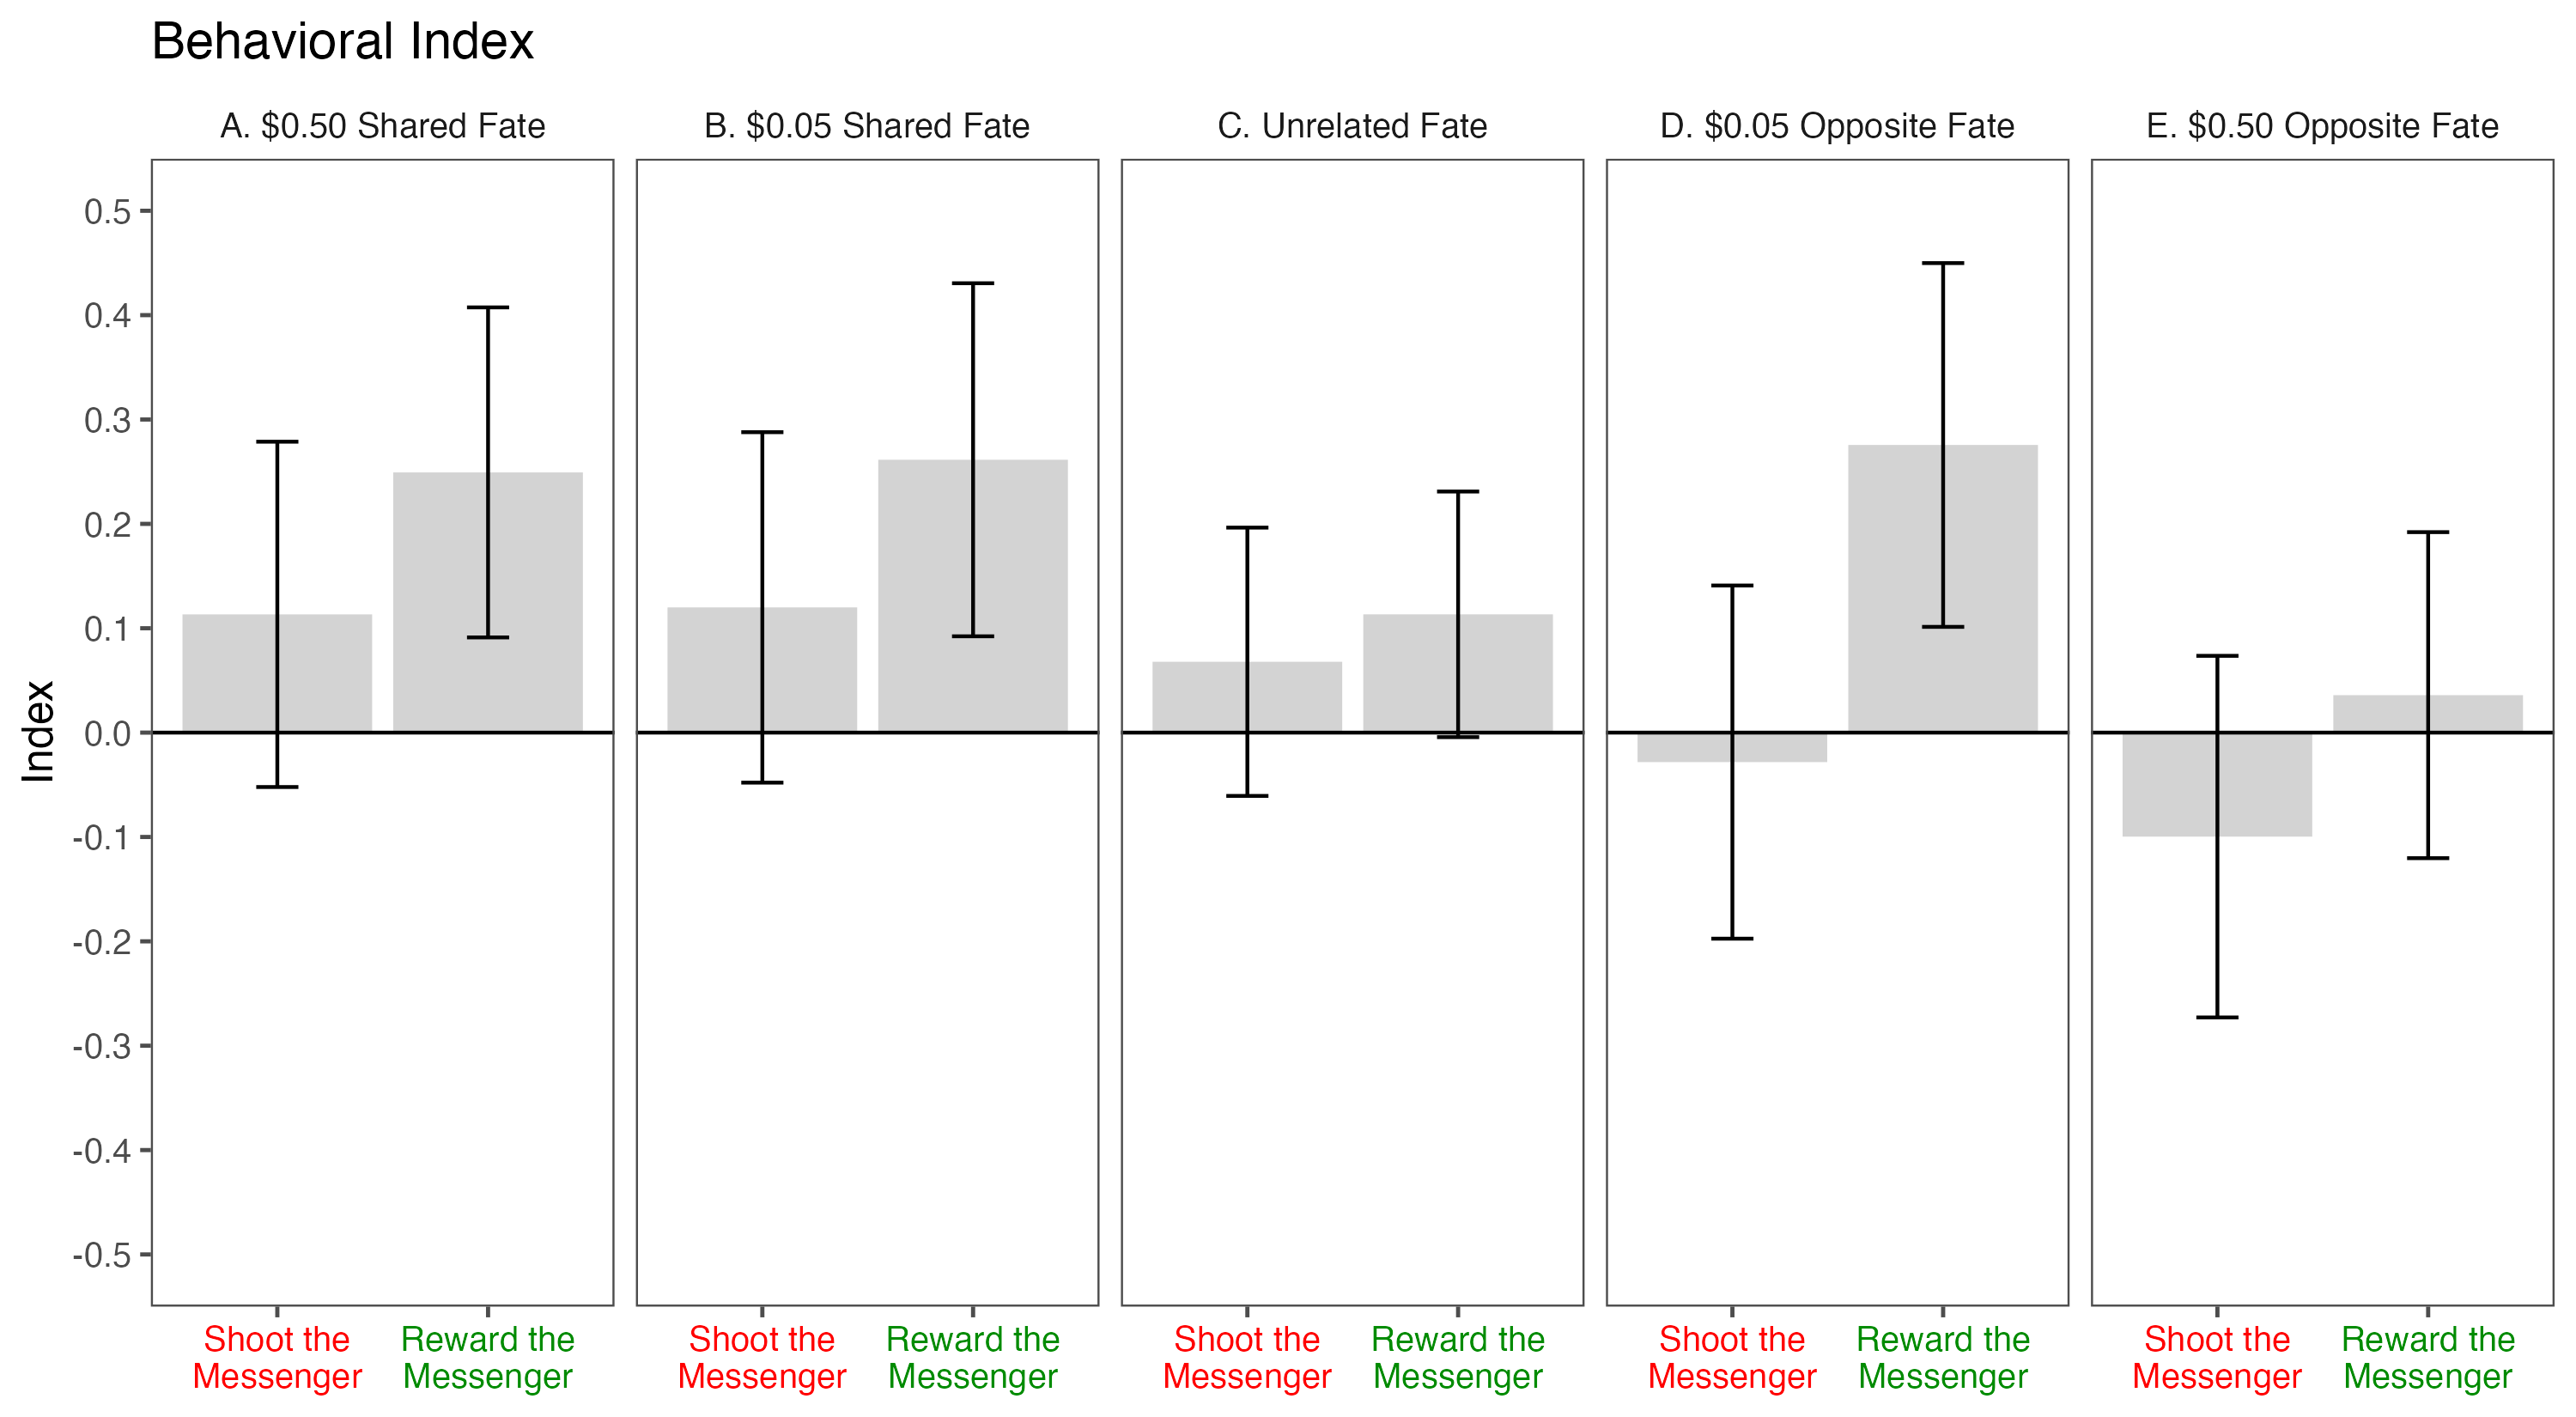
\includegraphics[width=1.0\textwidth]{figures/study2_main_fivecent_behavior_all.png}
  \caption{Difference in messenger and non-messenger ratings of the Behavioral Index by losing (STM) and winning (RTM) across Unrelated Fate, Shared Fate, Opposite Fate conditions, Study 2 (including 5 and 50 cent differences). 
  \textit{Note: OLS regression with robust standard errors, with error bars representing 95\% confidence intervals.In the behavioral index, the DV is calculated by averaging the standardized scores of the dictator game, spin the wheel task, and prisoner's dilemma. The \$0.05 Shared Fate (Panel A) and \$0.50 Shared Fate (Panel B) conditions are when the partner wins \$0.05 or \$0.50, respectively, when the respondent wins. The Unrelated Fate (Panel C) condition is when the partner winnings are unrelated to the respondent winning. The \$0.05 Opposite Fate (Panel D) and \$0.50 Opposite Fate (Panel E) conditions are when the partner wins \$0.05 or \$0.50, respectively, when the respondent loses.}}
  \label{fig:study2_main_fivecent_behavior_all}
\end{figure}%
\renewcommand{\baselinestretch}{1.67}%


\renewcommand{\baselinestretch}{1.25}%
\begin{figure}[!t]%
  \centering
  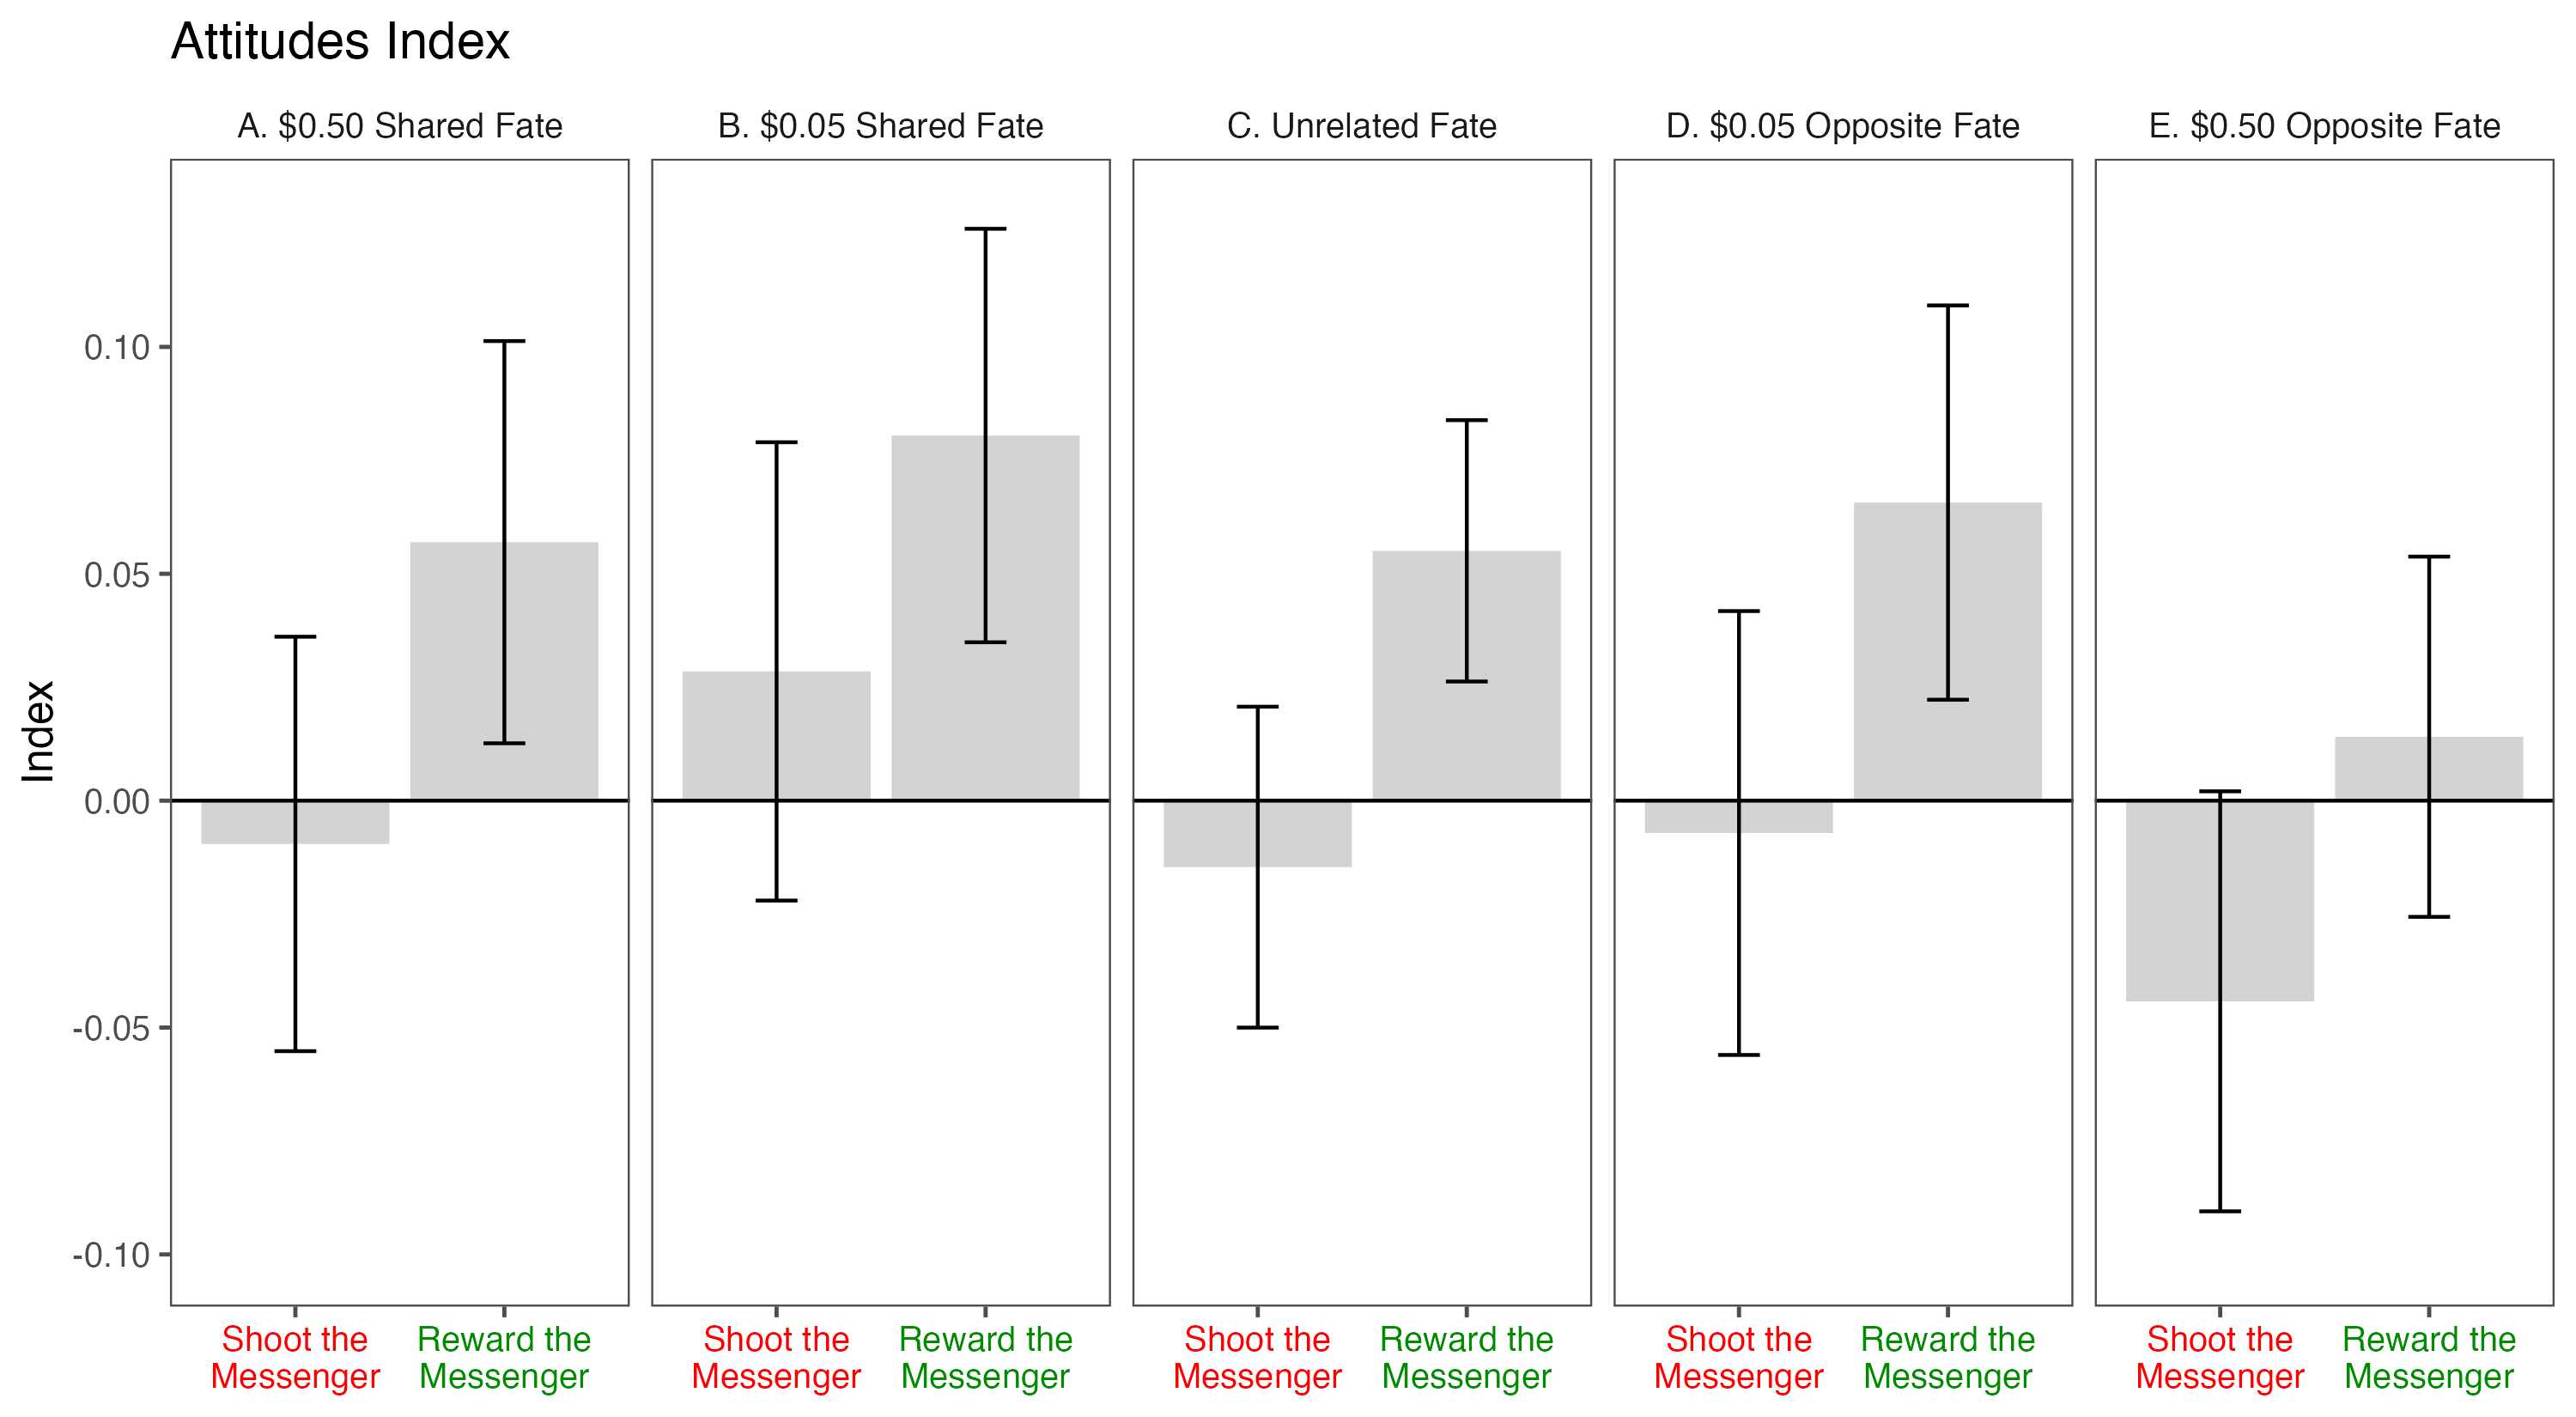
\includegraphics[width=1.0\textwidth]{figures/study2_main_fivecent_attitude_all.png}
  \caption{Difference in messenger and non-messenger ratings of the Attitudes Index by losing (STM) and winning (RTM) across Unrelated Fate, Shared Fate, Opposite Fate conditions, Study 2 (including 5 and 50 cent differences). 
  \textit{Note: OLS regression with robust standard errors, with error bars representing 95\% confidence intervals.In the attitudes index, the DV is calculated by averaging the ratings of the trustworthy, nice, likeable, and generous DVs to an index ranging from 0 to 1. The \$0.05 Shared Fate (Panel A) and \$0.50 Shared Fate (Panel B) conditions are when the partner wins \$0.05 or \$0.50, respectively, when the respondent wins. The Unrelated Fate (Panel C) condition is when the partner winnings are unrelated to the respondent winning. The \$0.05 Opposite Fate (Panel D) and \$0.50 Opposite Fate (Panel E) conditions are when the partner wins \$0.05 or \$0.50, respectively, when the respondent loses.}}
  \label{fig:study2_main_fivecent_attitude_all}
\end{figure}%
\renewcommand{\baselinestretch}{1.67}%


\clearpage

\section{Survey Questionnaires}

\subsection{Receiver Survey, Study 1}
\subsubsection*{1. Screeners}
\begin{itemize}
    \item Eggplant question
    \item IP-address screener
    \item Crime story
    \begin{itemize}
        \item Filter on the easy questions: How was the person caught? [He left his ID]
        \item Code whether they get the harder question right (how much \$ did person walk away with)
    \end{itemize}
\end{itemize}

\subsubsection*{2. Demographics}
Please answer these background questions about yourself. 

\begin{itemize}
    \item What is your age? [textbox]
    \item What is your sex? [Male / Female / Other / Prefer not to say]
    \item Generally speaking, do you consider yourself a: [Democrat / Republican / Independent / Other]
    \item (if Democrat/Republican:) Would you call yourself a strong [Democrat/Republican] or
    a not very strong [Democrat/Republican]? [Strong Democrat / Not very strong
    Democrat / Not very strong Republican / Strong Republican]

    (if Independent/Other:) Do you think of yourself as closer to the
    Democratic or the Republican Party? [Lean Democrat / Independent / Lean
    Republican]
    \item In general, how would you describe your own political viewpoint?
    [Very liberal / Liberal / Moderate / Conservative / Very conservative]
    \item What is the highest level of education you have completed? [No high
    school/High school graduate/Some college/2-year/4-year/Post-grad] 
    \item What
    is your employment status? [Full-time / Part-time / Temporarily laid off /
    Unemployed / Retired / Permanently disabled / Homemaker / Student / Other]
    \item What racial or ethnic group best describes you?
    [White / Black / Hispanic / Asian / Native American / Mixed / Other / Middle Eastern]
    \item Here are 7 statements about the world. Please indicate how much you
    disagree or agree with each statement by selecting the appropriate box. A
    score of 1 indicates you strongly disagree with a statement, while a score
    of 6 means you strongly agree with the item.   
    \begin{itemize}
	\item I basically feel that the world is a fair place.
	\item I feel that people get what they deserve.
	\item I feel that people get what they are entitled to have.
	\item I feel that a person's efforts are noticed and rewarded.
	\item I feel that people who meet with misfortune have brought it on themselves.
	\item I feel that rewards and punishments are fairly given.
	\item I feel that people earn the rewards and punishments they get.
	\end{itemize}
    \item Here are 5 statements about your personality. Please indicate how
    much each statement is characteristic of you by selecting the appropriate
    box. A score of 1 indicates that a statement is extremely uncharacteristic
    of you, while a score of 5 means that a statement is extremely
    characteristic of you.
    \begin{itemize}
	\item Some of my friends think I am a hothead.
	\item I have trouble controlling my temper.
	\item Sometimes I fly off the handle for no good reason.
	\item I sometimes feel like a powder keg ready to explode.
	\item When frustrated, I let my irritation show.
    \end{itemize}
    \item Here are 7 statements about you and the world. Please indicate how
    much you disagree or agree with each statement by selecting the appropriate
    box. A score of 1 indicates you strongly disagree with a statement, while a
    score of 6 means you strongly agree with the item.
    \begin{itemize}
    \item I believe in luck.
	\item Some people are consistently lucky, and others are unlucky.
	\item There is such a thing as luck that favors some people, but not others.
	\item I tend to win games of chance.
	\item Luck works in my favor.
	\item I consistently have good luck.
	\item I often feel like it's my lucky day.
\end{itemize}
\end{itemize}

\subsubsection*{Qualtrics Variables}
\begin{itemize}
\item \{\$Task1\} = \{``Prediction''/''Counting''\} 
\item \{\$Task1description\} = \{``coin toss''
/ ``number counting''\} 
\item \{\$Task1short\} = \{``predict the outcome of a coin toss
performed by the computer'' / ``count how many odd numbers are contained in a
table generated by the computer''\} 
\item \{\$Task1long\} = \{``Specifically, you will
select the ``Heads'' or ``Tails'' button and then the computer will flip a fair
coin that will turn up heads or tails with equal probability'' / ``Specifically,
you will select one of two options to indicate how many odd numbers are in the
table''\} 
\item \{\$Task1correct\} = \{``correctly predict the coin toss'' / ``correctly
count how many odd numbers are in the table''\} 
\item \{\$Task1observer\} = \{``your
prediction and the outcome of the coin toss'' / ``your count of how many odd
numbers are in the table''\} 
\item \{\$Task1noun\} = \{``prediction'' / ``count''\}
\item \{\$Task1CorrectMsg\} = (if emotionalMsg = 0) \{``Your coin toss prediction matched the coin toss. You
earned \$0.25.'' / ``Your count was correct. You earned \$0.25.''\} or 
(if emotionalMsg = 1) \{``Congratulations! You won!''\} 
\item \{\$Task1IncorrectMsg\} = (if emotionalMsg = 1) \{``Your coin toss prediction did not match the coin toss.
You did not earn a bonus.'' / ``Your count was incorrect. You did not earn a
bonus.''\} or (if emotionalMsg = 1) \{``Too bad! You lost!''\}
\item \{\$Task2PartnerLong\} = \{``the person who was the messenger from part 1'' / ``a
new human participant selected at random (not the messenger from part 1)''\}
\item \{\$Task2PartnerShort\} \{``the messenger from part 1'' / ``another participant''\}
\end{itemize}

\subsubsection*{3. Instructions}
Please read these instructions carefully. You will complete a brief
comprehension quiz after each part of these instructions and you will earn an
\textbf{additional 5 cent bonus} for each quiz question you get right. 

\begin{description}[listparindent = 1.5em]
\item[Overview Instructions] \hspace{1cm}

Today you will earn 50 cents for participating in this task. You
will also have the opportunity to earn additional money based on how you do on
quizzes about these instructions as well as your and other participants'
decisions. This additional money will be paid to you as an MTurk bonus in the
next two weeks. 

Today's task is divided into three parts. We will describe \textbf{part
1} now, and then tell you about \textbf{parts 2 and 3} later.
\end{description}

\subsubsection*{Part 1 Instructions: \{\$Task1\} task}

In \textbf{part 1}, you will be randomly paired
with another human participant in this task who has the role of \textbf{messenger}. 

You
will then perform a \textbf{\{\$Task1\} task} where you \{\$Task1short\}. \{\$Task1long\}. You
will have 15 seconds to make your decision.

The \textbf{messenger} will then tell you the
outcome of the \{\$Task1\} task. If you \{\$Task1Correct\}, you will earn an additional
\textbf{50 cent bonus}. Otherwise, you earn \textbf{nothing}. 

The \textbf{messenger} will observe
\{\$Task1observer\}. They will communicate the outcome to you by clicking a button
that sends a standard message with the result. The messenger can only send an
accurate message. 

Specifically, if your \{\$Task1noun\} is correct,
you will receive this message: 

\textbf{\{\$Task1CorrectMsg\}}

If your \{\$Task1noun\} is incorrect,you will receive this message: 

\textbf{\{\$Task1IncorrectMsg\}}

Once you have finished reading these instructions, please proceed to the
3-question comprehension quiz on the next screen. For each question you get
right, you will earn \textbf{5 cents}.

\begin{description}
\item[Part 1 Quiz Question 1] \hspace{1cm}
\begin{enumerate}
\item In part 1, you will \ldots
\begin{enumerate}
    \item spin the wheel. 
\item \{\$Task1short\}. 
    \item open a virtual door. 
    \item click as many times as you can in 15 seconds. 
\end{enumerate}
\end{enumerate}

Feedback: \{Correct/Incorrect.\} In part 1, you will \{\$Task1short\}.

\item[Part 1 Quiz Question 2] \hspace{1cm}
\begin{enumerate}
\setItemnumber{2}
\item In part 1 (after this quiz), how much of a bonus will you earn?
\begin{enumerate}
    \item Nothing. 
    \item \$0.50 no matter what. 
    \item It depends on whether you \{\$Task1correct\}.
    \item It depends on whether your partner decides to send you a bonus.
\end{enumerate}
\end{enumerate}

Feedback: \{Correct/Incorrect.\} Your part 1 bonus depends on whether you
\{\$Task1correct\}. If you do so, you will earn \$0.50.

\item[Part 1 Quiz Question 3] \hspace{1cm} 
\begin{enumerate} \setItemnumber{3}
\item How do you find out whether you \{\$Task1correct\}?
\begin{enumerate} 
\item The computer will alert me.
\item I will find out in a later task.
\item I will never find out.
\item Another participant, the messenger, will send me a message.    
\end{enumerate} 
\end{enumerate}

Feedback: \{Correct/Incorrect.\} Another participant, the messenger, will send
you a message that tells you whether you \{\$Task1correct\}.
\end{description}

\subsubsection*{Part 1, messenger assignment}

You have been matched to another participant in this survey who will be the
\textbf{messenger}. 

[insert messenger figure]

You will see this icon when you interact with or answer questions about the
\textbf{messenger}.

\subsubsection*{(if counting = 0) Part 1, predict a coin tosss}
The computer will next flip a fair coin that will turn up heads or tails with
equal probability. 

If you predict the coin toss, you will earn 50 cents.
Otherwise, you will earn nothing. 

Which side do you choose? Select the ``Heads''
or ``Tails'' button to continue. 

You have 15 seconds to decide or you cannot
earn a bonus.

\subsubsection*{(if counting = 1) Part 1, choose which figure has more dots}

\textbf{The Number Counting Task} 

On each of the next two screens, you will see one 6x6
grid filled with numbers. Your job is to count how many odd numbers are in each
grid and determine which of the two grids has more odd numbers. 

You will have 10
seconds to look at each grid, and 15 seconds to decide which of the two grids
contains more odd numbers. 

If you correctly identify the grid with the most odd
numbers, you will earn 50 cents. Otherwise, you will earn nothing. 

[Next screens:
Show one 6x6 grid per page] 

[Decision screen] Now we will verify whether you
counted the odd numbers correctly. 

Which grid contains the most odd numbers?

\subsubsection*{Part 1, message}

The
\textbf{messenger} has sent you this message: 

\{If correct\}: \{\$Task1CorrectMsg\}

\{If
incorrect\}: \{\$Task1IncorrectMsg\}

[Only for participants randomly assigned to answering the attitudes questions
toward the messenger right after Task 1]

\begin{itemize}
	\item Here are 4 statements about the \textbf{messenger}. Please indicate how much each
statement matches the messenger's traits by selecting the appropriate box. A
score of 1 indicates that the messenger does not have that trait at all, while a
score of 7 means that a trait describes the messenger extremely well.
\\
{[insert messenger figure]}
\begin{itemize}
    \item How trustworthy is the messenger? 
    \item How nice is the messenger? 
    \item How likeable is the messenger? 
    \item How generous is the messenger?
\end{itemize}

\item Now, thinking about the message that you received about your performance
in task 1, please indicate how much you feel each emotion by selecting the
appropriate box. A score of 0 indicates that you do not feel an emotion at all,
while a score of 10 means you feel an emotion very much.
\begin{itemize}
\item How angry does the message make you feel?
\item How sad does the message make you feel?
\item How happy does the message make you feel?
\item How enthusiastic does the message make you feel?
\item How confused does the message make you feel?
\item How indifferent does the message make you feel?
\end{itemize}
\end{itemize}

\subsubsection*{Part 2 Instructions}

[If assigned to the messenger]

Now it is time for \textbf{Part 2} of this task. 
    
    In part 2, you will play three
    games with \textbf{\{\$Task2PartnerLong\}}. 
    
    [insert figure of messenger]
    
    We will describe each of the three games before you play them and you
    will answer a quiz question after each page of instructions. Then you will
    have the chance to play each game for a bonus.

    We will tell you the outcome of each game when we will pay you for this
    survey. 
    
    Please read these instructions carefully. For each question you get
    right, you will earn \textbf{5 cents}.

    [If assigned to another participant]

    Now it is time for \textbf{Part 2} of this task. 
        
        In part 2, you will play three
        games with \textbf{\{\$Task2PartnerLong\}}. 
        
        [insert figure of participant]
        
        We will describe each of the three games before you play them and you
        will answer a quiz question after each page of instructions. Then you will
        have the chance to play each game for a bonus.
    
        We will tell you the outcome of each game when we will pay you for this
        survey. 
        
        Please read these instructions carefully. For each question you get
        right, you will earn \textbf{5 cents}.

\begin{description}[listparindent = 1.5em]
    \item[Allocation game:]  \hspace{1cm}
    
    In the allocation game, we will give you an extra \$.50. You will decide
    how to allocate this extra money. Specifically, you can keep it all, or you
    can give some or all of it to your partner. Any money you keep will be given
    to you as a bonus, while any money you share will be given to
    \{\$Task2PartnerShort\} as a bonus. 
    
    You will indicate your choice by moving a
    slider that shows how much you wish to give to your partner. 
    
    [Slider label:
    How much of your \$.50 do you wish to give to your partner,
    \{\$Task2PartnerShort?\}]
\end{description}

\begin{description}[listparindent = 1.5em]
    \item[Spin the wheel game:] \hspace{1cm}
    
In the spin the wheel game, you have the chance to win an additional
    \$0.50 if you predict the outcome of a wheel spin correctly.  
      
    The wheel has ten
    numbers and only one number is the winning one. You pick a number, and if
    the wheel stops at that number, you earn extra \$0.50. Otherwise, you do not
    earn any extra money. We will communicate to you the result of the wheel
    spin at the end of this task. 
    
    You cannot spin the wheel yourself, however.
    Instead, you have to decide who spins the wheel on your behalf. 
    
    Specifically,
    you will have to choose whether you want the computer or your partner,
    \{\$Task2PartnerShort\}, to spin the wheel. 
    
    Do you prefer that the computer or
    your partner, \{\$Task2PartnerShort\}, spin the wheel? 
    
    \{``Computer'' /
    ``Partner''\}
\end{description}

\begin{description}[listparindent = 1.5em]
    \item[Directions game:] \hspace{1cm} 
    
    In the directions game, you can win up to extra \$0.50 depending on the
    decisions that you and your partner, \{\$Task2PartnerShort\}, will make. 
    
    You and
    your partner must choose whether to go up or down. 
    
    If you choose to go \textbf{up}:
    
    \begin{itemize}
    	\item and your partner also chooses to go up, each of you gets \$0.40.
    	\item and your partner chooses to go down, you get nothing and your
    partner gets \$0.40.
    \end{itemize}

    If you choose to go \textbf{down}:
    
    \begin{itemize}
    	\item and your partner chooses to go up, you get \$0.40 and your partner
    gets nothing.
    	\item and your partner also chooses to go down, each of you gets \$0.10.
    \end{itemize}

    You and your partner will choose without knowing each other's choice.

    Which direction do you choose? 
    
    \{``Up'' / ``Down''\}

    \item[Part 2 Quiz Question 1] \hspace{1cm}
    \begin{enumerate}
        \item True or false: In part 2, you partner is
        \{\$Task2PartnerShort\}?
        \begin{enumerate}
            \item True
            \item False
        \end{enumerate}
    \end{enumerate}

    Feedback: \{Correct/Incorrect.\} In part 2, you partner is
    \{\$Task2PartnerLong\}.

    \item[Part 2 Quiz Question 2] \hspace{1cm}
    \begin{enumerate} \setItemnumber{2}
        \item In the allocation game, what happens to any of the \$.50 you decide to keep?
        \begin{enumerate}
            \item It is paid to me as a bonus.
            \item It is paid to my partner as a bonus.
            \item Nothing, it simply disappears.            
        \end{enumerate}
    \end{enumerate}

    Feedback: \{Correct/Incorrect.\} In part 2, any money you decide to keep
    is paid to you as a bonus, while any money you give to your partner is paid
    to them as a bonus.

    \item[Part 2 Quiz Question 3] \hspace{1cm}
    \begin{enumerate} \setItemnumber{3}
        \item In the spin the wheel game, who spins the wheel whose outcome you are trying to predict?
        \begin{enumerate}
            \item I spin the wheel.
            \item The computer always spins the wheel.
            \item My partner always spins the wheel.
            \item I decide whether the computer or my partner spins the wheel.                   
        \end{enumerate}
    \end{enumerate}

    Feedback: \{Correct/Incorrect.\} You decide whether your partner or the
        computer spins the wheel.

    \item[Part 2 Quiz Question 4] \hspace{1cm}
    \begin{enumerate}\setItemnumber{4}
        \item In the directions game, how much money do you and
        \{\$Task2PartnerShort\} earn if you choose to go up?
        \begin{enumerate}
            \item Each of you gets \$0.40 regardless of what \{\$Task2PartnerShort\} chooses. 
            \item If \{\$Task2PartnerShort\} also chooses to go up, each of you gets \$0.40. 
            \item You get nothing regardless of what \{\$Task2PartnerShort\} chooses.
            \item You get \$0.10 and \{\$Task2PartnerShort\} gets \$0.40.                      
        \end{enumerate}
    \end{enumerate}

    Feedback: \{Correct/Incorrect.\} If \{\$Task2PartnerShort\} also chooses to go up,
    each of you gets \$0.40.
\end{description}

Now it is time to play the games. The instructions for each game are displayed
again on each page for your convenience. 

[On each of the next three screens,
participants play the dictator game, the spin the wheel game, and the prisoner's
dilemma game.] 

[After playing the games, participants who have not yet received
the attitudes and emotions questions answer them]

\subsubsection*{Part 3}

Lastly, please answer the following questions about your experience in the first
two parts of this survey.

\begin{itemize}
    \item Now, think back about your \{\$Task1description\} task in part 1. How fair do you think the \{\$Task1description\} task was? [7-point scale
    from ``Not very fair'' to ``Very fair'']
    \item How accurate was the message
    about the \{\$Task1observer\} sent by the messenger? [7-point scale from ``Not
    accurate at all'' to ``Extremely accurate'']
    \item How likely is that the messenger was a real person? [7-point scale
    from ``Not likely at all'' to ``Extremely likely'']
    \item How likely is it that
    the coin toss outcome was revealed by a computer? [7-point scale from
    ``Not likely at all'' to ``Extremely likely'']
\end{itemize}

\subsubsection*{End}

Thank you for participating in this study. To receive your payment, please copy
and paste this unique ID into MTurk: 

[randomly generated 5-digit ID]

\clearpage
\subsection{Messenger Survey}

(Only the parts that are unique to the messenger survey are presented below)

\subsubsection*{Send Message Screen}

Now, please select the button below to send an important
message to another MTurk participant, \textbf{the receiver}.

[insert figure of the receiver]

Your message will be
truthful and could deliver good news or bad news to them. 

You have no control
over what message you can send. 

[Button: Send a message delivering good or bad
news to the receiver.]

\subsubsection*{Spin the Wheel Screen} 

Now, please select the button below to spin a wheel of
fortune on behalf of another MTurk participant, \textbf{the receiver}. 

[insert figure of the receiver]

You will not know
the outcome of the wheel spin. Based on the outcome of the wheel spin, another
MTurk participant may earn bonus money. 

[Button: Click this button to spin a
wheel on behalf of another participant.]

\clearpage
\subsection{Receiver Survey, Study 2}

(Only the parts that are unique to the Study 2 survey are presented below)

\subsubsection*{Variables}
\begin{itemize}
\item \{\$Task1\} = \{``Prediction'' / ''Counting''\} 
\item \{\$Task1description\} = \{``coin toss''
/ ``number counting''\} 
\item \{\$Task1short\} = \{``predict the outcome of a coin toss
performed by the computer'' / ``count how many odd numbers are contained in a
table generated by the computer''\} 
\item \{\$Task1long\} = \{``Specifically, you will
select the ``Heads'' or ``Tails'' button and then the computer will flip a fair
coin that will turn up heads or tails with equal probability'' / ``Specifically,
you will select one of two options to indicate how many odd numbers are in the
table''\} 
\item \{\$Task1correct\} = \{``correctly predict the coin toss'' / ``correctly
count how many odd numbers are in the table''\} 
\item \{\$Task1observer\} = \{``your
prediction and the outcome of the coin toss'' / ``your count of how many odd
numbers are in the table''\} 
\item \{\$Task1noun\} = \{``prediction'' / ``count''\}
\item \{\$Task1CorrectMsg\} = \{SEE BELOW\}
\item \{\$Task1IncorrectMsg\} = \{SEE BELOW\} 
\item \{\$Task2PartnerLong\} = \{``the
person who was the messenger from part 1'' / ``a new human participant selected
at random (not the messenger from part 1)''\} 
\item \{\$Task2PartnerShort\} \{``the
messenger from part 1'' / ``another participant''\} 
\item \{\$Instructions1\} = \{SEE
BELOW\}
\end{itemize}

\subsubsection*{\{\$Instructions1\}}

\begin{itemize}
\item -1 you will earn an additional 50 cents bonus and the messenger will not
earn any money for delivering this message. Otherwise, you earn nothing but the
messenger will earn a 50 cent bonus for delivering this message.

\item -0.1 you will earn an additional 50 cents bonus and the messenger will
not earn any money for delivering this message. Otherwise, you earn nothing but
the messenger will earn a 5 cent bonus for delivering this message.

\item 0 you will earn an additional 50 cent bonus and the messenger will not
earn any money for delivering this message. Otherwise, you earn nothing and the
messenger will not earn any money for delivering this message.

\item 0.1 you will earn an additional 50 cents bonus and the messenger will
earn a 5 cent bonus for delivering this message. Otherwise, you earn nothing and
the messenger will not earn any money for delivering this message.

\item 1 you will earn an additional 50 cents bonus and the messenger will earn
a 50 cent bonus for delivering this message. Otherwise, you will earn nothing
and the messenger will not earn any money for delivering this message.
\end{itemize}

\subsubsection*{\{\$Task1CorrectMsg\}}
\begin{itemize}
\item -1 ``Your coin toss prediction matched the coin toss. You earned \$0.50 but I
did not earn any money for delivering this message.'' / ``Your count was correct.
You earned \$0.50 but I did not earn any money for delivering this message.''

\item -0.1 ``Your coin toss prediction matched the coin toss. You earned \$0.50 but I
did not earn any money for delivering this message.''/ ``Your count was correct.
You earned \$0.50 but I did not earn any money for delivering this message.''

\item 0 ``Your coin toss prediction matched the coin toss. You earned \$0.50 but I did
not earn any money for delivering this message.''/ ``Your count was correct. You
earned \$0.50 and I did not earn any money for delivering this message.''

\item 0.1 ``Your coin toss prediction matched the coin toss. You earned \$0.50 and I
earned \$0.05 for delivering this message.'' / ``Your count was correct. You
earned \$0.50 and I earned \$0.05 for delivering this message.''

\item 1 ``Your coin toss prediction matched the coin toss. You earned \$0.50 and I
earned \$0.50 for delivering this message.'' / ``Your count was correct. You
earned \$0.50 and I earned \$0.50 for delivering this message.''
\end{itemize}

\subsubsection*{\{\$Task1IncorrectMsg\}}
\begin{itemize}
\item -1 ``Your coin toss prediction did not match the coin toss. You did not earn any
money but I earned \$0.50 for delivering this message.'' / ``Your count was
incorrect. You did not earn any money but I earned \$0.50 for delivering this
message.'' 

\item -0.1 ``Your coin toss prediction did not match the coin toss. You did
not earn any money but I earned \$0.05 for delivering this message.'' / ``Your
count was incorrect. You did not earn any money but I earned \$0.05 for
delivering this message.'' 

\item 0 ``Your coin toss prediction did not match the coin
toss. You did not earn any money and I did not earn any money for delivering
this message.''/ ``Your count was incorrect. You did not earn any money and I
did not earn any money for delivering this message.'' 

\item 0.1 ``Your coin toss
prediction did not match the coin toss. You did not earn any money and I did not
earn any money for delivering this message.''/ ``Your count was incorrect. You
did not earn any money and I did not earn any money for delivering this message.'' 

\item 1 ``Your coin toss prediction did not match the coin toss. You did not earn
any money and I did not earn any money for delivering this message.'' / ``Your
count was incorrect. You did not earn any money and I did not earn any money for
delivering this message.''
\end{itemize}

\subsubsection*{Part 1 Instructions: \{\$Task1\} task}

In \textbf{part 1}, you will be randomly paired
with another MTurk participant in this task who has the role of \textbf{messenger}. 

You 
will then perform a \textbf{\{\$Task1\} task} where you \{\$Task1short\}. \{\$Task1long\}. You
will have 15 seconds to make your decision. 

The \textbf{messenger} will then tell you the
outcome of the \{\$Task1\} task. 

If you \{\$Task1Correct\}, \{\$Instructions1\}.

Your partner will observe
\{\$Task1observer\}. They will communicate the outcome to you by clicking a
button that sends a standard message with the result. The messenger can only
send an accurate message.

Specifically, if your \{\$Task1noun\}
is correct, you will receive this message: \textbf{\{\$Task1CorrectMsg\}}. 

If your
\{\$Task1noun\} is incorrect, you will receive this message: \textbf{\{\$Task1IncorrectMsg\}}.

Once you have finished reading these instructions, please proceed to the
3-question comprehension quiz on the next screen. For each question you get
right, you will earn \textbf{5 cents}.

\begin{description}
\item[Part 1 Quiz Question 4] \hspace{1cm} 
\begin{enumerate} \setItemnumber{4}
\item How much does the messenger get paid for delivering this message?
\begin{enumerate}
\item The messenger [-1: earns a 50 cent bonus if you fail to \{\$Task1correct\} /
-0.1: earns a 5 cent bonus if you fail to \{\$Task1correct\} / 0: does not earn any
money for delivering this message / 0.1: earns a 5 cent bonus if you
\{\$Task1correct\} / 1: earns a 50 cent bonus if you \{\$Task1correct\}].
\item The messenger draws a card which reveals their payment.
\item I will never find out.
\item The messenger gets paid a fixed sum for delivering this message no matter what.
\end{enumerate} 
\end{enumerate}

Feedback: \{Correct/Incorrect.\} The messenger [-1: earns a 50 cent bonus if you
fail to \{\$Task1correct\} / -0.1: earns a 5 cent bonus if you fail to
\{\$Task1correct\} / 0: does not earn any money for delivering this message / 0.1:
earns a 5 cent bonus if you \{\$Task1correct\} / 1: earns a 50 cent bonus if you
\{\$Task1correct\}].

\end{description}

\subsubsection*{Part 3}

Now, think back about the game you just played. Suppose you were in the role of
the messenger rather than the receiver.

\begin{itemize}
    \item Do you think the receiver would like you more or less if you
    were the messenger who informed them that they \underline{lost}? 
    [5-point scale from ``The receiver would like me a lot less'' to ``The
    receiver would like me a lot more.''
    \item What makes you think so? [textbox]
    \item Do you think the receiver would like you more or less if you
    were the messenger who informed them that they \underline{won}? [5-point
    scale from ``The receiver would like me a lot less'' to ``The receiver would
    like me a lot more.''
    \item What makes you think so? [textbox]
    \item To what extent do you agree or disagree with the following statements:
    \begin{itemize}
        \item ``A messenger should be \textbf{rewarded} for delivering \textbf{good news} for
        which they are not responsible.'' [5-point scale from strongly agree to
        strongly disagree]
    \end{itemize}
    \begin{itemize}
    	\item ``A messenger should be \textbf{punished} for delivering \textbf{bad news} for which
    they are not responsible.'' [5-point scale from strongly agree to
    strongly disagree]
    \end{itemize}
\end{itemize}


\end{document}
